\documentclass[11pt,a4paper]{article}

% --- Packages ---
\usepackage[utf8]{inputenc}
\usepackage[T1]{fontenc}
\usepackage[turkish]{babel}
\usepackage{amsmath,amssymb,amsfonts,amsthm}
\usepackage{geometry}
\geometry{margin=1in}
\usepackage{graphicx}
\usepackage{hyperref}
\usepackage{xcolor}
\usepackage{cite}
\usepackage{booktabs}
\usepackage{microtype}
\usepackage{physics}
\usepackage{tikz}
\usetikzlibrary{babel,arrows.meta}

\usepackage{listings}

\hypersetup{
    pdftitle={Birleşik Büzülme Hipotezi ve Ölçek-Zaman Kalkülüsü: Genişlemeyen Bir Evrende Kozmoloji, Kütleçekim ve Dört Temel Etkileşimin Geometrik Külliyatı},
    pdfauthor={Muhammed Furkan Haydari},
    pdfsubject={Kuramsal Fizik, Doğa Felsefesi, Kozmoloji ve Kütleçekim},
    pdfkeywords={Birleşik Büzülme Hipotezi, Ölçek-Zaman Kalkülüsü, Konformal Kozmoloji, Nehir Modeli, 137 İnce Yapı Sabiti, Kuark Hapsi, CMB, Pantheon+},
    colorlinks=true,
    linkcolor=blue!70!black,
    citecolor=red!70!black,
    urlcolor=blue!80!black
}

% --- Listings Settings for Python Code ---
\definecolor{codegreen}{rgb}{0,0.55,0.2}
\definecolor{codegray}{rgb}{0.45,0.45,0.45}
\definecolor{codepurple}{rgb}{0.55,0.1,0.75}
\definecolor{codeblue}{rgb}{0.1,0.2,0.8}
\definecolor{backcolour}{rgb}{0.97,0.97,0.98}

\lstdefinestyle{pythoncode}{
    backgroundcolor=\color{backcolour},   
    commentstyle=\color{codegreen}\itshape,
    keywordstyle=\color{codeblue}\bfseries,
    numberstyle=\tiny\color{codegray},
    stringstyle=\color{codepurple},
    basicstyle=\ttfamily\scriptsize,
    breakatwhitespace=false,         
    breaklines=true,                 
    captionpos=b,                    
    keepspaces=true,                 
    numbers=left,                    
    numbersep=6pt,                  
    showspaces=false,                
    showstringspaces=false,
    showtabs=false,                  
    tabsize=2,
    frame=single,
    rulecolor=\color{gray!30},
    extendedchars=true,
    literate={ğ}{{\u{g}}}1 {ü}{{\"{u}}}1 {ş}{{\c{s}}}1 {ı}{{\i}}1 {ö}{{\"{o}}}1 {ç}{{\c{c}}}1
             {Ğ}{{\u{G}}}1 {Ü}{{\"{U}}}1 {Ş}{{\c{S}}}1 {İ}{{\.I}}1 {Ö}{{\"{O}}}1 {Ç}{{\c{C}}}1
             {²}{{$^2$}}1 {±}{{$\pm$}}1 {χ}{{$\chi$}}1 {Ω}{{$\Omega$}}1 {Λ}{{$\Lambda$}}1 {μ}{{$\mu$}}1 {ℓ}{{$\ell$}}1 {ϕ}{{$\phi$}}1
}
\lstset{style=pythoncode}

% --- Theorem Environments ---
\newtheorem{theorem}{Teorem}[section]
\newtheorem{definition}{Tanım}[section]
\newtheorem{axiom}{Aksiyom}[section]
\newtheorem{corollary}{Sonuç}[theorem]
\newtheorem{lemma}[theorem]{Lemma}
\newtheorem{remark}{Not}[section]

\title{\textbf{Birleşik Büzülme Hipotezi ve Ölçek-Zaman Kalkülüsü: \\ Genişlemeyen Bir Evrende Kozmoloji, Kütleçekim ve Dört Temel Etkileşimin Geometrik Külliyatı}}

\author{
    \textbf{Muhammed Furkan Haydari} \\
    \textit{Bağımsız Araştırma / Doğa Felsefesi ve Temel Fizik Üzerine Kavramsal Denemeler} \\
    \small ORCID: \href{https://orcid.org/0009-0003-2854-3947}{0009-0003-2854-3947} \quad$\bullet$\quad \small DOI: \href{https://doi.org/10.5281/zenodo.23633034}{10.5281/zenodo.23633034}
}

\date{\today}

\begin{document}
\shorthandoff{=}

\maketitle

\begin{abstract}
    Bu çalışmada, statik ve genişlemeyen bir arka plan uzay-zamanında yerel maddenin ölçek dinamikleri üzerinden doğadaki dört temel etkileşimi tek bir çerçevede yeniden formüle eden birleşik bir geometrik model öneriyoruz. Bu \textit{Birleşik Büzülme Hipotezi} çerçevesinde, kozmolojik kırmızıya kayma, yerel atomik yapıların değişmez arka plan metriğine göre sürekli ve ölçek-değişmez biçimde mekânsal olarak küçülmesinin ($r_{\mathrm{atom}}(t) \to 0$) doğrudan bir tezahürüdür. Konformal dönüşümler aracılığıyla, atomik ölçeklerdeki bu küçülmenin kozmik şişme veya karanlık enerji gibi varsayımlara ihtiyaç duymaksızın uzak gök cisimlerinin kırmızıya kaymasını ve zaman genişlemesini eksiksiz biçimde açıkladığını gösteriyoruz.

    Bu büzülme mekanizmasını alan gradyanlarına genişlettiğimizde, yerel kütle-enerjinin büzülmesinin çevreleyen vakum alan yoğunluğunda merkeze doğru sürekli bir koordinat akışı ve sürüklenme yarattığını ortaya koyuyoruz. Makroskopik sınırda bu vakum akışı kütleçekimin Painlev\'e--Gullstrand formülasyonunu tam olarak yeniden üretir; böylece yerçekimsel ivmelenme, yörünge mekaniği ve yerel büzülme/akış hızının ışık hızı $c$'yi aştığı olay ufuklarında ışığın hapsolması doğal biçimde açıklanır. Alt-atomik ölçeklerde ise elektronun çekirdeğe düşmesi problemi ölçek-değişmez bir asimptotik çekici olarak çözülür: elektron çekirdeğe doğru sarmal çizdikçe yerel uzunluk ölçekleri de orantılı olarak büzülür ve böylece ışımasal çöküş olmaksızın dinamik kararlılık korunur.

    Son olarak, elektrodinamiğin doğasını ve foton yayılımını ele alıyoruz. Elektromanyetik uyarılmaların temel olarak değişmez arka plan manifoldunun durağan yerel pertürbasyonları olduğunu; gözlemlenen ışık hızı $c$'nin ise doğrudan vakumun elastik faz iletim ve maddenin içsel kuantum faz tavan hızını nicellediğini ortaya koyuyoruz. Işığın yansıması, saçılması ve spektral algının bu büzülen gözlemci çerçevesinde nasıl çalıştığını matematiksel olarak formalize ederek, kütleçekimsel, elektromanyetik ve nükleer kuvvetlerin tek bir geometrik ölçek dinamiğine indirgenmesine yönelik kapsamlı bir yol haritası sunuyoruz.
\end{abstract}

\vspace{1em}
\noindent\textbf{Anahtar Kelimeler:} Birleşik Alan Teorisi, Konformal Kütleçekim, Büzülen Madde Kozmolojisi, Kozmolojik Kırmızıya Kayma, Painlev\'e--Gullstrand Metriği, Dalga Mekaniği, Durağan Vakum Elektrodinamiği.

\vspace{1em}
\hrule
\vspace{0.8em}
\tableofcontents
\vspace{0.8em}
\hrule
\vspace{1.5em}

% --- Modüler Bölümler ---
\section*{Epistemolojik Manifest: Kuramsal Paradigma Değişimi ve Doğa Felsefesi}
\addcontentsline{toc}{section}{Epistemolojik Manifest: Kuramsal Paradigma Değişimi ve Doğa Felsefesi}
\label{sec:epistemolojik_manifest}

\subsection*{1. Epistemolojik Sadelik ve Konformal Geometrik Perspektif}

Modern teorik fizikte ve gözlemsel kozmolojide karşılaşılan temel açık sorular—karanlık madde, karanlık enerji, kozmik şişme ve kuantum ölçekleri ile kütleçekim arasındaki kavramsal uyum—farklı kuramsal ve geometrik çerçevelerin araştırılmasını gerektirmektedir:
\begin{itemize}
    \item Galaksi dönüş eğrilerinin Keplerian dinamikten sapması, soğuk karanlık madde hipotezinin geliştirilmesine yol açmıştır.
    \item Tip Ia süpernovalarının parlaklık-kırmızıya kayma bağıntısı, kozmik ivmelenme ve karanlık enerji varsayımını doğurmuştur.
    \item Ufuk ve düzlük problemleri, erken evren kozmik enflasyon modellerini gündeme getirmiştir.
    \item Hadronların hapsi ve kütle kazanımı mekanizmaları ise perturbative olmayan alan teorilerinde araştırılmaya devam etmektedir.
\end{itemize}

Bu araştırma monografisi, metrik uzay genişlemesi yerine durağan bir arka planda maddesel bağlı yapıların yerel konformal ölçek büzülmesini ($r_{\mathrm{atom}}(t) \to 0$) ele alarak, bu gözlemsel olguların konformal simetri ve büzülen ölçüm standartları altında nasıl tezahür ettiğini incelemektedir. Bu yaklaşım, bilim felsefesinde Occam'ın usturası ilkesi doğrultusunda, asgari aksiyomatik varsayımla geniş bir gözlemsel spektrumun açıklanabilirliğini test etmeyi amaçlayan kuramsal bir araştırma programıdır.

\subsection*{2. Matematiksel Meşruiyet: Konformal İkizlik ve Nilpotent Cebir}

Uzayın genişlemesi ile atomik cetvellerin büzülmesi arasındaki ilişki bir soyutlama tercihinden ibaret kalmayıp, diferansiyel geometrinin kesin bir teoremine dayanır. Genel görelilikte metrik tensörün konformal dönüşümü:
\begin{equation}
    g_{\mu\nu} \to \Omega^2(t) g_{\mu\nu}
\end{equation}
koordinat sistemleri arasında tam bir geometrik eşdeğerlik (konformal ikizlik / conformal duality) kurar. Christof Wetterich (2013), Fred Hoyle, Jayant Narlikar ve Roger Penrose gibi kuramcıların farklı bağlamlarda işaret ettiği üzere; metrik uzayın genişlemesi ($a(t) \propto e^{H_0 t}$) ile maddesel uzunluk cetvellerinin daralması ($\lambda(t) \propto e^{-H_0 t}$) matematiksel olarak özdeş fiziksel öngörüler üretir.

Bu çalışmada geliştirilen $\kappa^2 = 0$ dual nilpotent cebir ve $\mathbb{D}_t \equiv \frac{d}{dt} + \kappa H_0$ Ölçek-Kovaryant Türevi, söz konusu konformal simetriyi pasif bir koordinat seçimi seviyesinden çıkararak nedensel ve dinamik bir fiziksel ontolojiye dönüştürmüştür. Uzay durağan Öklid sürekliliğini korurken, madde kendi içsel fazı boyunca büzülen dinamik bir Skalor olarak tanımlanmıştır.

\subsection*{3. Temel Sabitlerin Fiziksel Anlamı: $c$ ve Sommerfeld Sabiti $\alpha$}

Standart fizik, doğadaki temel boyutsuz ve boyutlu sabitlerin kökeni karşısında açıklamasız kalmış; bu değerleri evrenin başlangıcında belirlenmiş keyfi doğa sabitleri olarak kabul etmiştir:
\begin{itemize}
    \item \textit{``Işık hızı neden yaklaşık $3 \times 10^8\text{ m/s}$'dir ve neden doğanın aşılamaz mutlak tavanıdır?''}
    \item \textit{``Sommerfeld ince yapı sabiti $\alpha$'nın atomik kinematikteki fiziksel karşılığı nedir?''}
\end{itemize}

Bu çalışmada geliştirilen hidro-geometrik kalkülüs çerçevesinde:
\begin{enumerate}
    \item \textbf{Işık Hızı ($c$):} Harici bir hız limiti varsayımı olmaktan çıkarak, durağan elastik vakum dokusunun enine faz iletim hızı ($v_{\mathrm{faz}} = 1/\sqrt{\varepsilon_0\mu_0} = c$) ve bir vakum girdabı olan maddenin karakteristik radyal büzülme tavan hızı ($v_c = c$) olarak analitik temele kavuşturulmuştur.
    \item \textbf{İnce Yapı Sabiti ($\alpha \approx 1/137.036$):} Çekirdeğin içsel radyal büzülme hızı ($v_r = v_c = c$) karşısında, elektronun ışımasal çöküşe uğramadan kararlı bir yörüngede dolanabilmesi için çizdiği \textbf{geometrik spiral hatve oranıdır (vortex pitch ratio)}:
          \begin{equation}
              \alpha \equiv \frac{v_\theta}{v_r} = \frac{v_{\mathrm{Bohr}}}{c} = \frac{e^2}{4\pi\varepsilon_0\hbar c} \approx \frac{1}{137.036}.
          \end{equation}
          $Z\alpha \to 1$ eşiği ise teğetsel hızın büzülme tavanına ($v_\theta = c$) dayandığı ve süperkritik Dirac alanının vakum kutuplanmasıyla ($e^+ e^-$ çift üretimi) sistemi kararlı sınıra kilitlediği alt-atomik olay ufkudur.
\end{enumerate}
Bu iki temel sabitin hidrodinamik ve topolojik birer orana indirgenmesi, teorik fiziğin bir asırlık ontolojik kördüğümünü çözmektedir.

\subsection*{4. Boyutsuz Oranların Değişmezliği Kalkanı: Yerel Laboratuvar Testleri (Eötvös / MICROSCOPE)}

Birleşik Büzülme Hipotezi'nin yerel laboratuvar deneyleriyle uyumu, boyutsuz oranların korunumu ilkesiyle teminat altına alınmıştır. Eğer atomik cetveller kütle ölçeklemesinden yalıtılmış olarak tekil biçimde büzülseydi, MICROSCOPE uydu deneyi ve Eötvös burulma terazileri diferansiyel ivme sapmaları kaydederek teoriyi doğrudan yanlışlardı.

Bağlı tüm maddesel durumlar evrensel ölçek kuralı gereğince eş zamanlı olarak $m(t) = m_0 e^{H_0 t}$ konformal kütle kazandığından, laboratuvarda ölçülen herhangi iki kütlenin boyutsuz oranı mutlak olarak korunur:
\begin{equation}
    \frac{d}{dt} \left( \frac{m_{\mathrm{test}}}{m_{\mathrm{ref}}} \right) = \frac{d}{dt} \left( \frac{m_{1,0} e^{H_0 t}}{m_{2,0} e^{H_0 t}} \right) \equiv 0.
\end{equation}
Benzer biçimde İnce Yapı Sabiti $\alpha$ ve proton-elektron kütle oranı $\mu = m_p/m_e$ zamandan bağımsız kalır ($\dot{\alpha}/\alpha = 0, \dot{\mu}/\mu = 0$). Bu korunum, yerel Zayıf Eşdeğerlik İlkesi (WEP) testlerinin $\eta < 10^{-15}$ sınırında neden sıfır diferansiyel ivme ölçtüğünü tam bir tutarlılıkla açıklar.

\subsection*{5. Gökyüzü ile Yerkürenin Birleşimi: Yerel Ayrışma, Efemeris Sınırları ve Paleojeoloji}

Kozmolojik modeller sıklıkla milyarlarca ışık yılı uzaktaki soyut parametrelerle sınırlı kalarak yerel denetimden uzaklaşır. Birleşik Büzülme Hipotezi, derin uzay astrofiziği ile Güneş Sistemi yerel dinamiklerini tutarlı bir çerçevede birleştirir:
\begin{itemize}
    \item \textbf{Yerel Virial Ayrışma ve LLR Ölçümleri:} Kütleçekimsel potansiyelin baskın olduğu bağlı sistemlerde ($\nabla^2\Phi \gg 3H_0^2$), yerel yörüngeler McVittie kuralı uyarınca kozmik büzülme akışından virial olarak ayrışır. Apollo retroreflektörleriyle ölçülen Ay'ın $3.82\text{ cm/yıl}$'lık açılması, okyanus altimetrisiyle (TOPEX/Poseidon) doğrulanan gelgit sürtünmesi mekanizmasıyla tam bir uyum içindedir.
    \item \textbf{Efemeris ve Radar Sınırları:} Atomik saniyelerin büzülme ritmi yerel koordinatları değil atomik frekansları tanımladığından, gezegen efemerisleri ve radar telemetrisi (1 AU için $< 1.5\text{ cm/yıl}$) ile mutlak bir deneysel uyum sağlanır; kuram yerel gök mekaniği testlerinden başarıyla geçer.
\end{itemize}

\subsection*{6. Kavramsal Netlik: ``Vakum Akışkanı'' ve 19. Yüzyıl Eter Algısının Aşılması (Türeyen Uzay-Zaman)}

Modelde kullanılan ``vakum akışı'', ``girdap'' ve ``Bernoulli basıncı'' kavramları, 19. yüzyılın klasik mekanik eter hipotezleriyle karıştırılmamalıdır. Klasik eter teorileri uzayı sürtünmeli, mekanik dişlilerden oluşan maddesel bir sıvı olarak tasavvur etmiş ve Michelson--Morley deneyleriyle terk edilmiştir.

Bu çalışmada arka plan sürekliliği $\mathcal{E}_\infty$, sürtünmesiz, eylemsiz, kütlesiz ve mutlak pürüzsüz bir Öklid uzayıdır. Maddenin büzülmesiyle oluşan vakum akışı, modern kuramsal fizikteki \textit{Türeyen Uzay-Zaman (Emergent Spacetime)} ve \textit{Akustik/Hidrodinamik Yerçekimi (Analogue Gravity)} yaklaşımlarıyla tam bir metodolojik uyum sergiler. Parçacıklar durağan bir zemine gömülü harici bilyeler olarak değil; arka plan geriliminin topolojik girdap düğümleri olarak varlık kazanır.

\subsection*{7. Hesaplamalı Doğrulama ve Açık Kaynak Çözücüsü: Minimal CMB Kütüphanesi ve Sayısal Yol Haritası}

Birleşik Büzülme Hipotezi kavramsal ve analitik çerçevesini tamamlamakla kalmamış; Planck 2018 CMB tam açısal güç spektrumunu ($\ell = 2\text{--}2500$) fit eden açık kaynaklı, bağımsız araştırmacılarca tekrarlanabilir ve DOI tescilli minimal bir Python hesaplama çözücüsü (\texttt{scale-cmb-solver}, \href{https://github.com/FurkanHaydari/universe-is-not-expanding}{\texttt{FurkanHaydari/universe-is-not-expanding}}) ile somutlaştırılmıştır:
\begin{enumerate}
    \item \textbf{Planck CMB Açısal Güç Spektrumu Sayısal Çözücüsü:} Çalışmamızın minimal Python çözücüsü (\texttt{analysis/cmb\_spectrum\_analysis.py}); büzülen plazmanın duran dalga transfer denklemi, baryon yüklemesi ($R_b \approx 0.058$), akustik ölçek periyodu ($\Delta\ell \approx 293.5$), erken ISW potansiyel desteği ve Silk difüzyon sönümlemesi ($\ell_D \approx 1638.7$) mekanizmalarıyla Planck 2018 sıcaklık anizotropisi ($D_\ell^{\mathrm{TT}}$) verilerini (39 binned veri noktası) doğrudan modellemektedir. Çözücü; 1. Akustik Tepeyi $\ell_1 = 220.9$ (gözlem: 220.0), 2. Tepeyi $\ell_2 = 518.4$ (gözlem: 537.5), 3. Tepeyi $\ell_3 = 820.2$ (gözlem: 810.8) ve tepe oranlarını ($H_1/H_2 = 2.169$, $H_3/H_2 = 0.886$) Planck verileriyle tam bir ampirik uyumla üretmektedir. Bu minimal açık kaynak çekirdeği, standart CAMB ve CLASS algoritmalarının büzülen cetvel formatındaki tam Boltzmann hiyerarşisi simülatörüne genişletilmektedir.
    \item \textbf{Döteryum ve İlksel Bollukların Nükleer Ağ Simülasyonu:} Galaksiler arası gazda gözlenen $D/H \sim 2.5 \times 10^{-5}$ bolluk dengesi; yıldız içi astrasyon (döteryumun yanarak tükenmesi) ile durağan vakum akısı kaynaklı fotonükleer üretim mekanizmasının dengesini kuran çok bileşenli bir \textit{Astrofiziksel Nükleer Ağ Simülatörü} ile sayısal doğrulamaya kavuşturulmaktadır.
\end{enumerate}
Bu açık kaynaklı yazılım paketi, analitik mimarinin ampirik Planck ve Pantheon+ verileriyle doğrudan örtüştüğünü bilgisayar kodu seviyesinde tescil etmektedir.

\subsection*{8. Bilim Sosyolojisi ve Kurumsal Kabul Direnci}

Tarih boyunca bilimsel paradigmaların dönüşümü, Max Planck'ın işaret ettiği sosyolojik gerçeklikle ilerlemiştir: \textit{``Yeni bir bilimsel gerçek, muhaliflerin zamanla sahneden çekilmesi ve yeni neslin bu gerçeğe aşina olarak büyümesiyle zafer kazanır.''}

Bu çalışmanın muhatap olacağı asıl mukavemet, doğrudan kurumsal müesses nizamın (establishment) epistemolojik alışkanlıklarından kaynaklanacaktır:
\begin{itemize}
    \item Karanlık madde ve karanlık enerji varsayımlarının ortadan kalkması, bu alanlara ayrılmış devasa fonları ve onlarca yıllık kurumsal araştırma programlarını tartışmaya açacaktır.
    \item Tekil bir Büyük Patlama ($t=0$) tekilliğinin yerini maddenin büzülme fazı eşiğine bırakması, genişleyen metrik üzerine inşa edilmiş literatürün yeniden değerlendirilmesini gerektirecektir.
\end{itemize}
Bu nedenle çalışmamızda savunmacı bir polemik dili bütünüyle terk edilmiş; doğrudan tanımlar, analitik bağıntılar ve yanlışlanabilir somut öngörülerden oluşan aksiyomatik bir fizik mimarisi inşa edilmiştir. Doğa felsefesinin en yalın haliyle ortaya konan bu kuram, matematiksel ve gözlemsel testler karşısında tam bir tutarlılığa sahiptir.

\vspace{1.5em}
\hrule
\vspace{1.5em}

\section{Giriş}
\label{sec:giris}

Modern fizik, olağanüstü derecede başarılı fakat birbiriyle bağdaşmayan iki temel sütun üzerinde yükselmektedir: Kütleçekimi uzay-zamanın geometrik eğriliği olarak tanımlayan Genel Görelilik (GG) ve elektromanyetik, zayıf ve güçlü etkileşimleri eğri veya düz uzayda ayar teorileriyle açıklayan Standart Model. Yaklaşık bir asırlık yoğun teorik çabaya rağmen dört temel kuvvetin tek bir çatıda birleştirilmesi henüz başarılamamıştır. Eş zamanlı olarak, standart kozmolojik paradigma ($\Lambda$CDM), evrenin karanlık enerji ve erken dönem kozmik şişme (enflasyon) tarafından sürülen bir metrik genişleme içinde olduğunu varsaymaktadır.

Bu çalışmada alternatif bir temel önermeyi inceliyoruz: \textbf{Uzay-zaman arka planı bütünüyle statiktir; gözlemlenen kozmolojik ve kütleçekimsel fenomenler ise doğrudan maddenin sürekli ve ölçeğe bağlı olarak büzülmesinden kaynaklanmaktadır.}

Bu ikiliğin kavramsal kökleri konformal dönüşüm matematiğinde yer almaktadır (örneğin Wetterich~\cite{wetterich2013}, Hoyle ve Narlikar~\cite{hoyle1964}). $g_{\mu\nu} \to \Omega^2(t) \eta_{\mu\nu}$ konformal dönüşümü altında, parçacık kütlelerinin sabit olduğu genişleyen bir Friedmann--Lema\^itre--Robertson--Walker (FLRW) uzay-zamanı, parçacık kütlelerinin zamanla arttığı ve karakteristik kuantum uzunluklarının (Bohr yarıçapı $a_0 = \hbar^2/(m_e e^2)$ ve Compton dalga boyu $\lambda_C = \hbar/(mc)$) kozmik zaman boyunca küçüldüğü statik bir Minkowski uzay-zamanına matematiksel olarak birebir eşlenebilir:
\begin{equation}
      r_{\mathrm{atom}}(t) \propto \frac{1}{m(t)} \propto a(t)^{-1}.
      \label{eq:konformal_olcekleme}
\end{equation}

Bu noktada altı çizilmesi gereken en temel metodolojik ayrım şudur: Bu model, 1930'ların fotonun yolda enerji kaybettiğini varsayan klasik ve kusurlu ``Yorgun Işık'' (Tired Light) hipotezi veya statik uzayda durağan kalan Bondi--Gold modelleriyle özdeşleştirilemez. Konformal çerçevede geçmişe gidildikçe atomlar daha büyük olduğundan ($t \to -\infty \implies \lambda \to \infty$), geçmiş dönemde madde birbirinin içine geçmiş, optik derinliği aşırı yüksek ($\tau \gg 1$) ve termal dengeye (LTE) oturmuş yoğun bir plazma fazındadır. Yani standart $\Lambda$CDM'nin erken evren termodinamiği (CMB kara cisim ışıması ve nükleosentez dengesi), konformal ikililik sayesinde eksiksiz olarak muhafaza edilir.

Daha önceki konformal yaklaşımlar bu dönüşümü çoğunlukla matematiksel bir koordinat denkliği olarak ele almışken, biz madde büzülmesini hem kozmolojik ölçekleri hem de yerel etkileşimleri yöneten temel bir fiziksel ilke konumuna yükseltiyoruz.

\subsection{İncelenen Temel Fiziksel Sorular ve Geometrik Temalar}
\label{sec:temel_sorular}

Bu monografi, konformal ölçek-kovaryans ve büzülen ölçüm standartları çerçevesinde aşağıdaki temel fiziksel soruları ve araştırma temalarını analitik olarak incelemektedir:

\begin{enumerate}
      \item \textbf{Atomik Taban Durumunun Kararlılığı (Bohr Yarıçapı):} \\
            Klasik elektrodinamikte ivmelenen yükün Larmor ışımasıyla çekirdeğe çökmesi riski, kısa mesafelerde Heisenberg momentum belirsizliğinden türeyen kuantum kinetik basıncın ($E_{\mathrm{kin}} \propto 1/r^2$) çekici Coulomb potansiyelini ($-1/r$) dengelemesiyle giderilir; Ölçek-Zaman türevi ($\mathbb{D}_t(r/\lambda) = 0$) ise büzülen evrende bu taban durumunun konformal bir çekici olarak korunduğunu gösterir (Bölüm~\ref{sec:mikroskopik_kararlilik}).

      \item \textbf{Kütleçekimsel Potansiyel ve Zamanın Yavaşlaması:} \\
            Zaman, atomik sistemlerin büzülme sürecindeki kuantum faz evrimiyle parametrize edildiğinde ($dt = -d\ln\lambda/H_0$), kütleçekimsel vakum akıntı hızına ($v(r) = -\sqrt{2GM/r}$) karşı duran saatlerin akıntı direncine bağlı olarak $d\tau = dt\sqrt{1 - v^2(r)/c^2}$ biçiminde daha yavaş tıkırdaması incelenir (Bölüm~\ref{sec:buzulme_metrikleri}).

      \item \textbf{İnce Yapı Sabiti ($\alpha \approx 1/137.036$) ve Kinematik Hatve:} \\
            Boyutsuz Sommerfeld kuplaj sabiti $\alpha \approx 1/137.036$, elektronun teğetsel Bohr orbital hızı ($v_\theta \approx 2187\text{ km/s}$) ile vakumun içsel faz iletim tavan hızı ($v_c = c$) arasındaki \textbf{kinematik spiral hatve oranı} olarak değerlendirilir ($\alpha = v_{\mathrm{Bohr}} / v_c$). $Z\alpha \to 1$ rölativistik Dirac eşiği ise teğetsel hızın $c$'ye yaklaştığı alt-atomik sınır rejimine karşılık gelir (Bölüm~\ref{sec:olcek_kalkulusu_ana}).

      \item \textbf{Hubble Bağıntısının Kinematik Niteliği ($v = H_0 d$):} \\
            $v = H_0 d$ bağıntısı, kalkülüsün klasik çarpım kuralının $[(f\cdot g)' = f'g + fg']$ büzülen bir cetvele uygulanmasından doğan bir diferansiyel özdeşlik olarak ele alınır (Bölüm~\ref{sec:olcek_kalkulusu_ana}).

      \item \textbf{Kozmik Mikrodalga Arka Plan Işıması (CMB, 2.73 K) ve Termal Geçmiş:} \\
            CMB, geçmişte atomik ölçeklerin büyük olduğu ve maddenin yoğun plazma fazında bulunduğu dönemin akustik plazma rezonansları ve Kompaneets kinetiği ile yerel termodinamik dengeye (LTE) oturan ışıması olarak incelenir (Bölüm~\ref{sec:cmb_karanlik_madde}).

      \item \textbf{Kuantum Faz Kilitlenmesi ve İnterferometri Deneyleri:} \\
            Foton vakum faz dalgası olarak ele alındığında, ölçüm süreci dalganın detektör atomunun büzülme fazına kilitlenmesi (phase-pinning) olarak modellenir; kuantum silgisi deneylerinde ortogonal fazların yeniden mikslenmesiyle girişim deseni geri kazanılır (Bölüm~\ref{sec:kuantum_olcum_main}).

      \item \textbf{Hadronik Ölçek ve Kuark Hapsi Modeli:} \\
            Femtometre ölçeğinde ($r \sim 10^{-15}\text{ m}$) vakum akışının küresel seyreltiden 1-boyutlu silindirik tüpe geçişi incelenerek birim uzunluk geriliminin ($\sigma \approx 1\text{ GeV/fm}$) ve $V(r) = \sigma r$ lineer hapis potansiyelinin geometrisi modellenir (Bölüm~\ref{sec:nukleer_kuvvetler}).

      \item \textbf{Etkileşimlerin Efektif Boyutsal Akış Rejimleri:} \\
            Kütleçekim, Coulomb, hadronik hapis ve zayıf etkileşim potansiyelleri, tek bir boyutsal akış formülasyonunun ($(v/c)^2 = 2\mathcal{C}r^{-\gamma}$) farklı geometrik boyut indisleri ($\gamma = 1, -1, \text{exp}$) altında karşılaştırmalı olarak ele alınır (Bölüm~\ref{sec:nukleer_kuvvetler}).

      \item \textbf{Kiral Ölçekleme Dinamiği ve Baryon Asimetrisi:} \\
            Tek yönlü evrensel büzülme akışının ($\dot{\lambda} < 0$) tanımladığı zaman oku ($dt = -d\ln\lambda/H_0$), kiral simetri kırınımı dinamiklerinin ve sağ kiral nükleonların kararlılığının incelenmesine kuramsal zemin sağlar (Bölüm~\ref{sec:olcek_kalkulusu_ana}).

      \item \textbf{Temel Büyüklüklerin Parametrik İlişkisi:} \\
            Zaman ($t$), konum ($\mathbf{x}$), kütle ($m$) ve faz hızı ($c$) parametrelerinin, maddenin ölçek parametresi ($\lambda(t)$) ve ölçek-zaman kalkülüsü dahilinde ortak bir çerçevede nasıl ilişkilendirilebileceği incelenir (Bölüm~\ref{sec:ontolojik_indirgeme}).
\end{enumerate}

\subsection{Ontolojik Zorunluluk: Dört Temel Postulatın Tek Bir Mekanizmada Eritilmesi}
\label{sec:ontolojik_indirgeme}

Modern teorik fiziğin (Genel Görelilik ve Standart Model) en derin kavramsal tıkanıklığı, doğayı tanımlarken kullandığı dört temel sütunu birbirinden bütünüyle bağımsız ve bağlantısız birer aksiyom (postulat) olarak kabul etmesidir:
\begin{enumerate}
      \item \textbf{Zaman ($t$):} Kendi başına akan dördüncü bir koordinat boyutu veya kuantum durumlarının üzerinde evrildiği dışsal bir skaler parametre olarak postüle edilir.
      \item \textbf{Konum / Uzay ($\mathbf{x}$):} Maddenin içinde yer aldığı ya bükülen bir zemin (Genel Görelilik) ya da kuantum alanlarının üzerinde dalgalandığı eylemsiz bir sahne olarak postüle edilir.
      \item \textbf{Kütle ($m, M$):} Parçacıklara ya dışarıdan atanan bir eylemsizlik katsayısı ya da Higgs mekanizmasıyla keyfi Yukawa bağlaşımları üzerinden kazandırılan bir özellik olarak postüle edilir.
      \item \textbf{Işık Hızı ($c$):} Evrenin mutlak hız sınırı ve nedensellik sabiti olarak postüle edilir.
\end{enumerate}

Bu dört büyüklük birbirinden kopuk primitifler olarak kaldığı sürece, bunların türevleri olan dört temel kuvvetin (Kütleçekim, Elektromanyetizma, Güçlü ve Zayıf Nükleer) tek bir çatıda birleştirilmesi epistemolojik olarak imkansızdır. Kütleçekim uzay-zamanı bükerken, kuantum alanları sabit uzay-zaman üzerinde ayar simetrileri işletir; zaman kuantumda mutlak, görelilikte dinamiktir.

\textbf{Birleşik Büzülme Hipotezinin ve bu çalışmanın temel felsefi ve matematiksel iddiası şudur:}
\textit{Dört temel kuvveti tek bir formülde eritebilmek için, evvela bu kuvvetlerin ifade edildiği zaman, konum, kütle ve ışık hızı kavramlarının kendileri tek bir ortak parametrenin ve fiziksel mekanizmanın farklı tezahürleri olarak çözülmelidir!}

Modelimizde bu ortak temel parametre, \textbf{Maddenin Durağan Vakumdaki Ölçek Dinamiği ($\lambda(t)$ ve Büzülme Jeneratörü $\kappa$)}'dır:
\begin{itemize}
      \item \textbf{Işık Hızı ($c$):} Vakumun serbest elastik dalga iletim hızı ile vakum girdabı olan maddenin karakteristik kuantum faz hızını ($v_c = 1/\sqrt{\varepsilon_0\mu_0} = c$) niceler.
      \item \textbf{Zaman ($t$):} Atomların kendi içine büzüşürken kaydettiği logaritmik kuantum faz günlüğüdür ($dt \equiv -\frac{1}{H_0} d\ln\lambda$).
      \item \textbf{Konum / Uzaklık ($R$):} Statik arka plan noktası $\mathbf{X}_0$'ın büzülen atomik cetvele $\lambda(t)$ bölünmesiyle türeyen boyutsuz bir orandır ($R(t) = \mathbf{X}_0 / \lambda(t)$).
      \item \textbf{Kütle ($M$):} Vakum akışının ivme alanının (hız gradyanının) kapalı bir yüzey boyunca net akısıdır ($M \equiv \frac{1}{4\pi G} \oint_{\partial \Omega} |(\mathbf{v}_{\mathrm{inflow}} \cdot \nabla) \mathbf{v}_{\mathrm{inflow}}| \, dA$).
\end{itemize}

Bu dört temel kavram tek bir parametrede ($\lambda(t)$) eritildiğinde, dört temel kuvvet artık farklı ve uzlaştırılamaz alanlar olmaktan çıkar; tek bir evrensel vakum akış denkleminin ($(v/c)^2 = 2\mathcal{C}r^{-\gamma}$) farklı geometrik boyut ($\gamma=1, -1$) ve doyum hallerindeki doğal yansımalarına dönüşür.


\section{Mevcut Fizikteki Standart Metrik Sistem}
\label{sec:standart_metrik}

Modern teorik fizik, uzay-zamanın geometrisini ve dinamiklerini tanımlamak için Riemann geometrisine dayalı metrik tensör formülasyonunu ($g_{\mu\nu}$) kullanır. Çizgisel diferansiyel uzunluk elemanı genel olarak şu şekilde ifade edilir:
\begin{equation}
    ds^2 = g_{\mu\nu} dx^\mu dx^\nu.
    \label{eq:genel_cizgi_elemani}
\end{equation}

Standart fizikte temel yapı taşını oluşturan üç kritik metrik sistemi bulunmaktadır:

\subsection{Düz Uzay-Zaman (Minkowski Metriği)}
Özel görelilikte, kütleçekimin ve eğriliğin bulunmadığı eylemsiz referans sistemleri Minkowski metriği $\eta_{\mu\nu} = \mathrm{diag}(-1, 1, 1, 1)$ ile tanımlanır:
\begin{equation}
    ds^2 = -c^2 dt^2 + dx^2 + dy^2 + dz^2 = -c^2 dt^2 + dr^2 + r^2 d\Omega^2,
    \label{eq:minkowski_metrik}
\end{equation}
burada $d\Omega^2 = d\theta^2 + \sin^2\theta d\phi^2$ açısal çizgisel elemandır. Bu metrikte $c$, kütlesiz elektrodinamik uyarımların (fotonların) mutlak boşluktaki değişmez yayılma hızı olarak kabul edilir; koordinat ızgarası ise rijit ve zamandan bağımsız varsayılır.

\subsection{Genişleyen Evren Metriği (FLRW)}
Standart $\Lambda$CDM kozmolojisinde, evrenin homojen ve izotropik olduğu varsayımı altında Friedmann--Lema\^itre--Robertson--Walker (FLRW) metriği kullanılır:
\begin{equation}
    ds^2 = -c^2 dt^2 + a^2(t) \left[ \frac{dr^2}{1 - kr^2} + r^2 d\Omega^2 \right],
    \label{eq:flrw_metrik}
\end{equation}
burada $a(t)$ zamana bağlı boyutsuz kozmik ölçek faktörü, $k \in \{-1, 0, 1\}$ ise uzaysal eğrilik parametresidir. Düz bir evren için ($k=0$):
\begin{equation}
    ds^2 = -c^2 dt^2 + a^2(t) d\mathbf{x}^2.
    \label{eq:flrw_duz}
\end{equation}
Standart yorumda, koordinat uzaklığı sabit kalan iki galaksi arasındaki fiziksel mesafe $R(t) = a(t) r$ zamanla artar. Uzak gök cisimlerinden gelen ışığın kırmızıya kayması ($z$), fotonun genişleyen uzay dokusu boyunca seyahat ederken dalga boyunun metrik tarafından gerilmesiyle açıklanır:
\begin{equation}
    1 + z = \frac{\lambda_{\mathrm{goz}}}{\lambda_{\mathrm{yay}}} = \frac{a(t_0)}{a(t_e)}.
    \label{eq:standart_redshift}
\end{equation}

\subsection{Kütleçekimsel Eğrilik Metriği (Schwarzschild ve Painlev\'e--Gullstrand)}
Dönmeyen, yüksüz ve küresel simetrik bir $M$ kütlesinin yarattığı uzay-zaman eğriliği standart olarak Schwarzschild koordinatlarında ifade edilir:
\begin{equation}
    ds^2 = -\left(1 - \frac{2GM}{c^2 r}\right) c^2 dt^2 + \left(1 - \frac{2GM}{c^2 r}\right)^{-1} dr^2 + r^2 d\Omega^2.
    \label{eq:schwarzschild_standart}
\end{equation}
Bu metrik, sonsuzdan serbest düşüşe geçen bir gözlemcinin öz zamanı ($dt_{\mathrm{ff}} = dt + \frac{\sqrt{2GM/r}}{c(1 - 2GM/c^2 r)} dr$) cinsinden ifade edildiğinde Painlev\'e--Gullstrand koordinat formuna dönüşür~\cite{painleve1921, gullstrand1922}:
\begin{equation}
    ds^2 = -c^2 dt_{\mathrm{ff}}^2 + \left( dr + \sqrt{\frac{2GM}{r}} dt_{\mathrm{ff}} \right)^2 + r^2 d\Omega^2.
    \label{eq:painleve_standart}
\end{equation}
Bu formülasyon kütleçekimin ``uzay nehri'' (river of space) modelini oluşturur: statik arka plan Öklid ızgarası ($\mathbf{X}_0$) yerinde sabit kalırken, vakum dokusundaki skaler faz akısı kütle merkezine doğru $v_{\mathrm{akis}}(r) = \sqrt{2GM/r}$ hızıyla içeri çekilmektedir (tıpkı bakır telin yerinde durması ama içinden elektrik akımının akması gibi).


\section{Birleşik Büzülme Hipotezi: Büzülme Hızı (\texorpdfstring{$v_c$}{vc}) ve Metriklerin Yeniden İnşası}
\label{sec:buzulme_metrikleri}

Mevcut fizikteki bu metrik yapıları tersine çevirerek uzay dokusunun genişlemediği, aksine maddenin büzüldüğü gerçeğinden yola çıkıyoruz.

\subsection{Işık Hızı Yerine ``Büzülme Hızı'' (\texorpdfstring{$v_c$}{vc}) Sabiti}
Standart fizikte $c$ sabiti ışığın boşluktaki hızı olarak postüle edilir. Biz ise şu temel aksiyomu ortaya koyuyoruz:

\begin{quote}
    \textbf{Aksiyom 1 (Vakum Faz Yayılımı ve Maddenin İçsel Kuantum Faz Hızı):}
    Statik arka plan uzayı ve vakum dokusu mutlak olarak durağandır ($\mathbf{v}_{\mathrm{uzay}} = 0$). Foton, durağan vakum dokusunun komşu hücreleri arasındaki serbest enine elastik gerilim dalgasıdır ($v_{\mathrm{trans}} = 0$). Bu faz dalgası statik Öklid uzayı boyunca vakumun karakteristik iletim hızı $v_{\mathrm{faz}} = 1/\sqrt{\varepsilon_0\mu_0}$ ile koordinat kat ederek yayılır.

    Madde ise vakumun kendi kapalı topolojik girdap düğümü (Skalor Düğümü) olduğundan, atomik ölçekteki karakteristik kuantum faz salınımı ve rölativistik sınır hızı ($v_c$) vakum ortamının bu karakteristik faz iletim hızıyla özdeşleşir:
    \begin{equation}
        v_c \equiv \frac{1}{\sqrt{\varepsilon_0\mu_0}} = c \approx 2.99792 \times 10^8 \text{ m/s}.
        \label{eq:buzulme_hizi_tanim}
    \end{equation}
    Burada iki temel hız rejiminin birbirinden kesin olarak ayırt edilmesi zorunludur:
    \begin{enumerate}
        \item \textbf{İçsel Kuantum Faz Hızı ($v_c = c$):} Vakumun elastik faz iletim hızı ve atomik girdabın içsel rölativistik dönüş tavanıdır ($c \approx 3 \times 10^8\text{ m/s}$).
        \item \textbf{Kozmolojik Ölçek Daralma Hızı ($|\dot{r}_{\mathrm{atom}}| = H_0 r_{\mathrm{atom}}$):} Atomun fiziksel yarıçapının evrensel asırlık küçülme temposudur ($|\dot{r}_{\mathrm{atom}}| \approx (2.3 \times 10^{-18}\text{ s}^{-1}) \times (10^{-10}\text{ m}) \approx 2.3 \times 10^{-28}\text{ m/s}$). Bu hız $c$'den 36 mertebe ($10^{36}$) daha küçüktür; atomlar bu sayede anında sıfıra çökmeyip milyarlarca yıl boyunca kararlılıklarını muhafaza ederler.
    \end{enumerate}
    Büzüşen atomik cetvel ve saatlerimizle ölçtüğümüzde, vakum dokusunda ilerleyen bu serbest faz dalgasının yayılma hızını kendi içsel kuantum faz tavan hızımıza bağıl olarak tam $c$ olarak kaydederiz ($v_{\mathrm{faz}} = v_c = c$). Kozmolojik kırmızıya kayma, durağan vakumda sabit dalga boyuna sahip bu salınımı algılayan atomik cetvellerimizin asırlık büzüşmesinden ($r_{\mathrm{atom}}(t) \to 0$) kaynaklanır.
\end{quote}

Böylece temel uzay-zaman çizgisel elemanımız değişmez arka plan koordinatlarında ($\mathbf{x}, t$) daima düz kalır:
\begin{equation}
    d\Sigma^2 = -v_c^2 dt^2 + d\mathbf{x}^2.
    \label{eq:statik_arkaplan_metrigi}
\end{equation}

\subsection{Kozmolojik Metrik: Genişleyen Uzay Yerine Büzülen Atom Metriği}
Uzay koordinatları $\mathbf{x}$ geni\c{s}lemez ($d\mathbf{x} = \text{sabit}$). Ancak bir gözlemcinin kullandığı tüm ölçüm standartları (atomik cetveller $r_{\mathrm{atom}}$) zamanla büzülür. Boyutsuz atomik ölçek fonksiyonunu tanımlayalım:
\begin{equation}
    \lambda(t) \equiv \frac{r_{\mathrm{atom}}(t)}{r_{\mathrm{atom}}(t_0)} = \frac{1}{a(t)}, \quad \lambda(t_0) = 1.
    \label{eq:olcek_fonksiyonu}
\end{equation}
Büzülme hızı logaritmik türev ile verilir:
\begin{equation}
    \frac{\dot{\lambda}(t)}{\lambda(t)} = -H_0.
    \label{eq:buzulme_hubble}
\end{equation}

Büzülen bir atomik cetvelle ölçülen diferansiyel uzunluk $d\mathbf{x}_{\mathrm{goz}}$ ile arka plan koordinatı $d\mathbf{x}$ arasındaki bağıntı:
\begin{equation}
    d\mathbf{x}_{\mathrm{goz}} = \frac{d\mathbf{x}}{\lambda(t)} \implies d\mathbf{x} = \lambda(t) d\mathbf{x}_{\mathrm{goz}}.
    \label{eq:cetvel_donusumu}
\end{equation}
Bu bağıntıyı statik arka plan metriğine~\eqref{eq:statik_arkaplan_metrigi} yerleştirdiğimizde:
\begin{equation}
    d\Sigma^2 = -v_c^2 dt^2 + \lambda^2(t) d\mathbf{x}_{\mathrm{goz}}^2.
    \label{eq:buzulen_cetvel_metrigi}
\end{equation}
Kendi cetvelinin büzüldüğünün farkında olmayan ve cetvelini ``sabit'' kabul eden yerel bir gözlemcinin algıladığı etkin metrik $ds_{\mathrm{etkin}}^2 = \lambda^{-2}(t) d\Sigma^2$ konformal yeniden ölçeklemesiyle elde edilir:
\begin{equation}
    ds_{\mathrm{etkin}}^2 = -\frac{v_c^2}{\lambda^2(t)} dt^2 + d\mathbf{x}_{\mathrm{goz}}^2 = -v_c^2 d\tau^2 + a^2(\tau) d\mathbf{x}_{\mathrm{statik}}^2,
    \label{eq:etkin_flrw}
\end{equation}
burada $d\tau = \lambda^{-1}(t) dt = a(t) dt$ konformal kozmolojik zamandır.

\textbf{Matematiksel Sonuç:} Standart $\Lambda$CDM modelindeki FLRW metriği, statik bir Minkowski uzayında büzülen atomik cetvellerle yapılan gözlemin birebir konformal izdüşümüdür. Kırmızıya kayma ($z$), geçmişte ($t_e$) daha büyük olan atomların daha düşük frekansta foton salmasının doğrudan bir sonucudur:
\begin{equation}
    1 + z = \frac{\nu_{\mathrm{referans}}}{\nu_{\mathrm{gelen}}} = \frac{m(t_0)}{m(t_e)} = \frac{r_{\mathrm{atom}}(t_e)}{r_{\mathrm{atom}}(t_0)} = \frac{\lambda(t_e)}{\lambda(t_0)}.
    \label{eq:bizim_redshift}
\end{equation}

\begin{quote}
    \small
    \textbf{Kavramsal Netlik (Boş Uzay vs. Ölçülen Mesafe):} \\
    Burada altı çizilmesi gereken en temel epistemolojik ayrım şudur: Uzayın kendisi mutlak olarak durağan, metriksiz ve pürüzsüz bir Öklid sürekliliğidir ($\mathcal{E}_\infty$). Kendi başına metre veya saat barındırmaz. Algıladığımız tüm ``boşluk'' ve ``mesafeler'', büzüşen atomik cetvellerimizin o sabit aralığa sığma sayısını ($N = |\mathbf{X}_0|/r_{\mathrm{atom}}$) ifade eder. Atomlar küçüldükçe araya daha çok atom sığar ve gözlemci uzayın genişlediği yanılsamasına kapılır (Bölüm~\ref{sec:zaman_konum_turetilis_main}, Teorem~\ref{thm:konum_uzaklik_turetilis_main}).
\end{quote}

\subsection{Kütleçekimsel Vakum-Akış Metriği ve Süreklilik Denklemi}
Madde kütlesi $M$, trilyonlarca büzülen atomun oluşturduğu yerel bir yoğunluk merkezidir. Atomların sürekli kendi içlerine büzülmesi, çevreleyen statik vakum alanından merkeze doğru radyal bir akış debisi (inflow velocity) doğurur.

\subsubsection{Varyasyonel Temel: 3+1 ADM Eylemi ve Düz Uzayda Nehir Hızının Türetilişi}
\label{sec:adm_eylem_turetilis}
Nehir Modelindeki vakum akış hızı $v(r) = -\sqrt{2GM/r}$ keyfi bir benzetim veya sezgisel bir hipotez değildir; **düz uzay kısıtı altındaki Einstein-Hilbert gravitasyon eyleminin doğrudan varyasyonel extremumudur (Euler--Lagrange çözümüdür).**

Genel Görelilikte uzay-zaman metriği Arnowitt--Deser--Misner (ADM) 3+1 biçiminde ayrıştırılır:
\begin{equation}
    ds^2 = -\left(N^2 - \beta_i \beta^i\right) v_c^2 dt^2 + 2 \beta_i v_c dt dx^i + \gamma_{ij} dx^i dx^j,
    \label{eq:adm_metrik_ayrisim}
\end{equation}
burada $N$ lapse fonksiyonu, $\boldsymbol{\beta}$ shift vektörü ve $\gamma_{ij}$ 3-boyutlu uzaysal metriktir.

Birleşik Büzülme Hipotezinin temel aksiyomu uyarınca arka plan uzayı Öklid sürekliliğidir ve eğrilmez; dolayısıyla uzaysal metrik ve lapse fonksiyonu şu kesin kısıtları sağlar:
\begin{equation}
    \gamma_{ij} = \delta_{ij} \quad (\text{Düz Öklid Uzayı}, \; R^{(3)} = 0), \qquad N = 1 \quad (\text{Düzgün Zaman Adımı}).
    \label{eq:duz_uzay_kisit}
\end{equation}
Bu geometrik kısıtlar altında yerçekimi alanının tek bağımsız dinamik serbestlik derecesi, vakum akış hızıyla orantılı olan shift vektörüdür:
\begin{equation}
    \boldsymbol{\beta}(\mathbf{r}) \equiv -\frac{\mathbf{v}_{\mathrm{vakum}}(\mathbf{r})}{v_c}.
    \label{eq:shift_vektor_tanim}
\end{equation}
Bu kesit üzerinde dışsal eğrilik tensörü ($K_{ij}$) shift gradyanları ile tanımlanır:
\begin{equation}
    K_{ij} \equiv \frac{1}{2N} \left( \nabla_i \beta_j + \nabla_j \beta_i \right) = -\frac{1}{2 v_c} \left( \partial_i v_j + \partial_j v_i \right), \qquad K \equiv K^i_i = -\frac{1}{v_c} \nabla \cdot \mathbf{v}.
    \label{eq:dissal_egrilik_shift}
\end{equation}

Einstein--Hilbert yerçekimi eylemi $S_{\mathrm{EH}} = \frac{v_c^3}{16\pi G} \int d^4x \sqrt{-g} R$, ADM ayrışımında ve düz uzay ($\gamma_{ij} = \delta_{ij}, R^{(3)} = 0$) kısıtı altında indirgendiğinde:
\begin{equation}
    S_{\mathrm{grav}}[\mathbf{v}] = \frac{v_c^3}{16\pi G} \int dt d^3x \left( K_{ij} K^{ij} - K^2 \right) + S_{\mathrm{madde}}[\mathbf{v}],
    \label{eq:adm_grav_eylem}
\end{equation}
haline gelir. Küresel simetrik ve durağan bir radyal akışta ($\mathbf{v} = v(r) \hat{\mathbf{r}}$), dışsal eğrilik bileşenleri:
\begin{equation}
    K_{rr} = -\frac{1}{v_c} \frac{dv}{dr}, \qquad K_{\theta\theta} = K_{\phi\phi} = -\frac{1}{v_c} \frac{v(r)}{r},
\end{equation}
olup eylem yoğunluğunun kinetik terimi:
\begin{equation}
    K_{ij} K^{ij} - K^2 = -\frac{2}{v_c^2} \left( \frac{v}{r} \frac{dv}{dr} + \frac{v^2}{r^2} \right) = -\frac{1}{v_c^2 r^2} \frac{d}{dr}\left( r v^2 \right).
    \label{eq:kinetik_egrilik_ozdeslik}
\end{equation}
formuna sadeleşir. Noktasal bir durağan $M$ kütlesi için eylemin varyasyonu ($\delta S / \delta v(r) = 0$) hesaplandığında:
\begin{equation}
    \frac{\delta S_{\mathrm{grav}}}{\delta v(r)} = 0 \implies \nabla \cdot \left( v \frac{dv}{dr} \hat{\mathbf{r}} \right) = -4\pi G M \delta^3(\mathbf{r}).
    \label{eq:varyasyon_akis_sonuc}
\end{equation}
Bu diferansiyel denklemin integrali alındığında doğrudan:
\begin{equation}
    v(r) \frac{dv(r)}{dr} = -\frac{GM}{r^2} \implies \frac{1}{2} \frac{d}{dr}\left( v^2(r) \right) = -\frac{GM}{r^2}.
\end{equation}
Sonsuzlukta durgunluk sınır şartı ($v(\infty) = 0$) uygulandığında, radyal akış hız fonksiyonu analitik kesinlikle çıkar:
\begin{equation}
    \mathbf{v}_{\mathrm{vakum}}(r) = -\sqrt{\frac{2GM}{r}} \hat{\mathbf{r}}.
    \label{eq:vakum_cekis_hizi}
\end{equation}
\textbf{Varyasyonel Sonuç:} Painlevé--Gullstrand vakum akış hızı, **düz Öklid uzayında yaşayan bir shift vektör alanının Einstein eylemini minimize eden tekil analitik extremumudur.**

\subsubsection{Vakum Nereye Gider? Nilpotent Yutak ve Boşluk Diverjansının Geometrik Anlamı}
Klasik akışkan dinamiğinde içe doğru sürekli akan bir akışkan merkezde birikmek veya sonsuz yoğunluk tekilliği ($\rho \to \infty$) üretmek zorundadır. Burada iki ayrı rejim kesin olarak ayırt edilmelidir:
\begin{enumerate}
    \item \textbf{Boş Uzay Rejimi ($r > 0, \rho_M = 0$):} Painlevé--Gullstrand hız alanının düz Öklid sürekliliğindeki diverjansı:
    \begin{equation}
        \nabla \cdot \mathbf{v}_{\mathrm{vakum}} = \frac{1}{r^2} \frac{\partial}{\partial r}\left( r^2 \left(-\sqrt{\frac{2GM}{r}}\right) \right) = -\frac{3}{2} \sqrt{\frac{2GM}{r^3}} = - v_c K,
        \label{eq:extrinsic_curvature_trace}
    \end{equation}
    değerini verir. Bu diverjans, boşlukta fiziksel bir akışkan maddesinin aniden yok olması anlamına gelmez; 3+1 ADM geometrisinde sabit zaman yapraklarının dışsal eğriliğinin izine ($K \equiv K^i_i = -\frac{1}{v_c}\nabla\cdot\mathbf{v}$, Denklem~\ref{eq:dissal_egrilik_shift}) karşılık gelir. Düz uzay koordinat ızgarasının kütleçekim merkezine doğru konformal olarak sıkışma temposunu niceler.
    \item \textbf{Maddesel Çekirdek ve Nilpotent Yutak ($r \to 0, \rho_M \neq 0$):} Akışın fiziksel olarak maddeyle etkileştiği çekirdek havzasında ise süreklilik denklemi, nilpotent büzülme jeneratörü $\kappa$ ($\kappa^2 = 0$) üzerinden tanımlı bir nilpotent yutak (\textit{nilpotent sink}) ile dengelenir:
    \begin{equation}
        \nabla \cdot \mathbf{v}_{\mathrm{fiziksel}} = -4\pi G \rho_M \kappa = \mathcal{S}_{\mathrm{sink}}.
        \label{eq:sureklilik_main}
    \end{equation}
    Merkeze ulaşan 3-boyutlu uzaysal vakum akısı, uzay koordinatları içinde yığılmaz. $\kappa^2 = 0$ cebirsel kuralı uyarınca uzaysal hacim boyutunu kaybederek doğrudan maddenin içsel kuantum faz frekansına ($\omega = M c^2 / \hbar$) ve içsel ölçek büzülme hızına ($\dot{\lambda} = -H_0 \lambda$) dönüştürülür. Böylece Einstein Genel Göreliliğindeki karadelik tekillikleri ($r=0$) ortadan kalkar; merkez, uzaysal akışın içsel kuantum saat frekansına dönüştüğü dinamik bir faz sınırıdır.
\end{enumerate}

Arka plan vakumu $\mathcal{E}_\infty$, sonsuz ve ölçeksiz bir sürekliliktir. Homojen bir evrende her atomun oluşturduğu radyal debi, çevreleyen tüm atomların simetrik akısıyla global olarak dengelenir ($\sum \mathbf{v}_{\mathrm{inflow}} = 0$); dolayısıyla vakumun basıncı ve elastik gerilimi evrensel ölçekte tükenmeden mutlak olarak korunur.

Bu vakum akışının içinde bulunan bir test parçacığının veya dalganın hissettiği metrik doğrudan çizgisel kayma ile yazılır:
\begin{equation}
    ds^2 = -v_c^2 dt^2 + \left( dr - v_{\mathrm{vakum}}(r) dt \right)^2 + r^2 d\Omega^2.
    \label{eq:bizim_vakum_metrigi}
\end{equation}
Parantezi açtığımızda:
\begin{equation}
    ds^2 = -\left(1 - \frac{v_{\mathrm{vakum}}^2(r)}{v_c^2}\right) v_c^2 dt^2 - 2 v_{\mathrm{vakum}}(r) dt dr + dr^2 + r^2 d\Omega^2.
    \label{eq:vakum_metrik_acik}
\end{equation}
Bu denklemde $v_{\mathrm{vakum}}(r) = -\sqrt{2GM/r}$ yerleştirildiğinde:
\begin{equation}
    ds^2 = -\left(1 - \frac{2GM}{v_c^2 r}\right) v_c^2 dt^2 + 2\sqrt{\frac{2GM}{r}} dt dr + dr^2 + r^2 d\Omega^2.
    \label{eq:bizim_yercekimi_tam}
\end{equation}

\paragraph{3D Düz Dilimler ve 4D Riemann Eğriliği (Gauss--Codazzi Özdeşliği):}
Painlevé--Gullstrand koordinatlarında uzaysal dilimlerin Öklid metriğine sahip olması ($\gamma_{ij} = \delta_{ij}$, $^{(3)}R \equiv 0$), uzay-zamanın düz olduğu anlamına gelmez. 4-boyutlu eğrilik, 3+1 ADM Gauss--Codazzi bağıntısı ($^{(4)}R = K_{ij}K^{ij} - K^2$) gereği doğrudan dışsal eğrilik tensörü ($K_{ij} = -\frac{1}{2c}(\partial_i v_j + \partial_j v_i)$) tarafından üretilir. Bu tensörün ürettiği Kretschmann eğrilik skaları $\mathcal{K} \equiv R^{\alpha\beta\gamma\delta} R_{\alpha\beta\gamma\delta} = \frac{48 G^2 M^2}{c^4 r^6}$ tam olarak Schwarzschild eğriliğini verir. Dolayısıyla Nehir Modeli, 4-boyutlu uzay-zaman eğriliğinin durağan bir Öklid arka planındaki akışkan hız gradyanı ve kayma tensörü cinsinden analitik bir tasviridir.

\subsection{Vakum Akışında İvmelenme Mekanizması: Neden Sabit Hızla Değil de \texorpdfstring{$g$}{g} ile Düşeriz?}
\label{sec:ivmelenme_ispat}

Nehir Modeline yöneltilebilecek en haklı ve temel fizik sorusu şudur:
\textit{``Eğer kütleçekim maddenin vakumu içine çekmesinden ibaretse, Dünya'ya doğru düşen bir cisim neden nehirde sabit hızla sürüklenmeyip sürekli ivmelenir ($a = g \approx 9.8\text{ m/s}^2$)? Sabit bir akıntı ivme üretemez; ivmelenmenin matematiksel ve fiziksel kökeni nedir?''}

Bu soru, akışkanlar mekaniğindeki yerel ivme ile konvektif ivme arasındaki ayrım ve küresel daralma geometrisiyle eksiksiz çözülür:

\subsubsection{1. Akış Hızı Neden Sabit Değildir? (Küresel Boğaz Daralması)}
Dünya'nın $r$ yarıçapındaki eşmerkezli küresel kabuk alanı $A(r) = 4\pi r^2$'dir. Sonsuzlukta durgun olan bir vakum akışkanının merkeze doğru enerji korunumu ($\frac{1}{2} v^2 - \frac{GM}{r} = 0$) veya sıkıştırılamaz Euler sürekliliği altında daralan küresel kabuktan geçiş hızı:
\begin{equation}
    v_{\mathrm{inflow}}(r) = -\sqrt{\frac{2GM}{r}} \hat{\mathbf{r}}.
    \label{eq:akis_hizi_tekrar}
\end{equation}
Geniş bir ovadan dar bir kanyona giren nehrin hızlanması gibi; uzayda $r$ azaldıkça ($r \to 0$), vakum akış hızı $r^{-1/2}$ ile orantılı olarak \textbf{sürekli artar}.
\begin{itemize}
    \item Ay yörüngesinde ($r \approx 384\,400\text{ km}$): Vakum akış hızı yalnızca $v \approx 1.44\text{ km/s}$'dir.
    \item Dünya yüzeyinde ($r = R_\oplus \approx 6371\text{ km}$): Vakum akış hızı tamı tamına:
          \begin{equation}
              |v_{\mathrm{inflow}}(R_\oplus)| = \sqrt{\frac{2GM_\oplus}{R_\oplus}} \approx 11.186\text{ km/s}
              \label{eq:kurtulma_hizi_ispat}
          \end{equation}
          değerine ulaşır. Bu değer, Dünya'nın rölativistik \textbf{kurtulma hızına (escape velocity)} özdeştir.
\end{itemize}

\subsubsection{2. Euler Konvektif İvmesi ve \texorpdfstring{$g = GM/r^2$}{g = GM/r\texttwosuperior{}} İspatı}
Akışkanlar mekaniğinde akıntıya bırakılan bir test parçacığının maruz kaldığı toplam ivme maddesel türev (Euler konvektif ivmesi) ile hesaplanır:
\begin{equation}
    \mathbf{a} = \frac{D\mathbf{v}}{Dt} = \underbrace{\frac{\partial \mathbf{v}}{\partial t}}_{\text{Yerel İvme (Zamanla Değişim)}} + \underbrace{(\mathbf{v} \cdot \nabla)\mathbf{v}}_{\text{Konvektif İvme (Konumla Değişim)}}.
    \label{eq:maddesel_turev}
\end{equation}
Dünya'nın kütlesi zamandan bağımsız durağan olduğundan akış alanı kararlıdır ($\frac{\partial \mathbf{v}}{\partial t} = 0$). Fakat serbest bırakılan bir taş aşağı doğru düştükçe, nehrin daha yavaş aktığı bir irtifadan nehrin daha hızlı aktığı bir irtifaya girer. Parçacığın hissettiği radyal ivme:
\begin{equation}
    a_r(r) = v(r) \frac{dv(r)}{dr}.
    \label{eq:konvektif_ivme_tanim}
\end{equation}
Hız fonksiyonunun radyal türevini adım adım alalım:
\begin{align}
    v(r)          & = -\sqrt{2GM} \, r^{-1/2}, \label{eq:adim1}                                                               \\
    \frac{dv}{dr} & = -\sqrt{2GM} \left( -\frac{1}{2} r^{-3/2} \right) = \frac{1}{2} \sqrt{2GM} \, r^{-3/2}. \label{eq:adim2}
\end{align}
Şimdi bu iki ifadeyi Denklem~\eqref{eq:konvektif_ivme_tanim}'de çarpalım:
\begin{align}
    a_r(r) & = \left( -\sqrt{2GM} \, r^{-1/2} \right) \cdot \left( \frac{1}{2} \sqrt{2GM} \, r^{-3/2} \right) \nonumber \\
           & = -\frac{1}{2} (2GM) \, r^{-1/2 - 3/2} \nonumber                                                           \\
           & = -GM \, r^{-2} = \mathbf{-\frac{GM}{r^2}}.
    \label{eq:g_ispat_sonuc}
\end{align}
Dünya yüzeyinde ($r = R_\oplus$):
\begin{equation}
    a_r(R_\oplus) = -\frac{GM_\oplus}{R_\oplus^2} = -g \approx -9.807\text{ m/s}^2.
\end{equation}
\textbf{Matematiksel ve Fiziksel Sonuç:} Kütleçekimsel ivme ($g$), \textbf{merkeze doğru daralan küresel uzayda hızlanan bir vakum akışkanının konvektif hız gradyanıdır ($v \frac{dv}{dr}$)}.

\subsubsection{3. Yeryüzünde Duran Bir Gözlemci Neden Ağırlık ($W = mg$) Hisseder?}
Serbest düşüşteki bir asansörde bulunan bir gözlemci sıfır yerçekimi (ağırlıksızlık) yaşar; çünkü vakum nehriyle birlikte aynı konvektif ivmeyle sürüklenmektedir ($a_{\mathrm{net}} = 0$).

Yeryüzünde duran bir gözlemcinin nehir boyunca serbestçe sürüklenmesi zemin tarafından engellenir. Bu esnada durağan vakum dokusu, uzaydan gelip Dünya'nın merkezine doğru gözlemcinin vücudundaki her bir atomun içinden tam \textbf{$11.2\text{ km/s}$ hızla akıp gitmektedir!}

Zeminin gözlemciyi sabit tutmak için uyguladığı yukarı yönlü normal tepki kuvveti:
\begin{equation}
    N = m \cdot \left( v \left|\frac{dv}{dr}\right| \right) = m \cdot \frac{GM}{r^2} = mg.
\end{equation}
Böylece tartıya çıktığınızda okunan $70\text{ kg}$ ağırlık; **ayaklarınızın altından Dünya'nın merkezine doğru $11.2\text{ km/s}$ hızla hücum eden vakum akışının hız gradyanına karşı durma direncinizdir!**

\subsubsection{4. Gezegensel Yörünge Kararlılığı: Esir Sürtünmesi Neden Yoktur? ($\eta = 0$)}
Güneş çevresinde dönen gezegenlerin akan vakum nehrinde sürtünme (aether drag) yaşayarak Güneş'e düşmemesi iki temel ilkeye dayanır:
\begin{enumerate}
    \item \textbf{Sıfır Viskoziteli İdeal Süper-Akışkan ($\eta = 0$):} Vakum dokusunda moleküler serbest yol veya iç sürtünme viskozitesi ($\eta$) bulunmaz. Akış tamamen dağılmasızdır (dissipationless).
    \item \textbf{Painlev\'e--Gullstrand Metriğinin Hamiltonyen Korunumu:} Denklem~\eqref{eq:bizim_yercekimi_tam}'deki çizgisel eleman, Schwarzschild metriğinin bir koordinat transformasyonu olduğundan; gezegenlerin serbest düşüş jeodezikleri Schwarzschild yörüngeleriyle \textbf{matematiksel olarak özdeştir}. Açısal momentum ($L = r^2 \dot{\phi} = \text{sabit}$) kesin biçimde korunur; teğetsel sürtünme terimi ($\mathbf{F}_{\mathrm{drag}} = 0$) özdeş olarak sıfırdır.
\end{enumerate}

\subsubsection{5. Işığın Kütleçekimsel Sapması: Einstein'ın ``2 Katı'' Çarpanı (\texorpdfstring{$\Delta\theta = 4GM/c^2 b$}{4GM/c2b})}
Standart fizikte ışığın kütleçekimsel sapması, Newtonian çekimin öngördüğü değerin ($\Delta\theta_{\mathrm{Newton}} = \frac{2GM}{c^2 b}$) tam 2 katıdır. Nehir modelimizde $ds^2 = 0$ ışık çizgisi için koordinat entegrasyonu yapıldığında bu 2 katlık çarpan iki ayrı fiziksel etkinin toplamından türer:
\begin{enumerate}
    \item \textbf{Radyal Akış Sürüklenmesi (1. Kat):} Fotonun vakum nehrinin radyal akış hızına ($v(r) = \sqrt{2GM/r}$) maruz kalmasından kaynaklanan çizgisel sürüklenme ($\Delta\theta_1 = \frac{2GM}{c^2 b}$).
    \item \textbf{Kırılma İndisi Gradyanı ve Fermat İlkesi (2. Kat):} Merkeze doğru hızlanan akış, arka plan vakumunda etkin bir optik kırılma indisi gradyanı oluşturur:
          \begin{equation}
              n(r) = \frac{c}{c - |v(r)|} \approx 1 + \sqrt{\frac{2GM}{c^2 r}} + \frac{GM}{c^2 r}.
          \end{equation}
          Huygens--Fermat dalga cephesi prensibi uyarınca, dalga cephesinin kütleye yakın olan iç kenarı daha yavaş ilerlerken dış kenarı daha hızlı ilerler. Bu optik kırılma gradyanı tamı tamına ikinci bir $\Delta\theta_2 = \frac{2GM}{c^2 b}$ sapması üretir.
\end{enumerate}
İki katkı toplandığında toplam sapma açısı:
\begin{equation}
    \Delta\theta_{\mathrm{toplam}} = \Delta\theta_1 + \Delta\theta_2 = \frac{4GM}{c^2 b}
    \label{eq:sapma_tam_ispat}
\end{equation}
olarak uzay bükülmeksizin, Einstein'ın Genel Görelilik sonucu ile analitik bir uyum içinde elde edilir.

\subsection{Olay Ufku ve Işığın Karadelikten Kaçamayışının Mekanizması}
Standart fizikte karadelik olay ufku, uzayın geometrik eğriliğinin sonsuza ıraksadığı bir tekillik bölgesi olarak yorumlanır. Hipotezimizde ise bu durum son derece yalın bir akışkan dinamiğine indirgenir:

Radyal olarak dışarı doğru kaçmaya çalışan bir ışık dalgasının net koordinat hızı:
\begin{equation}
    \frac{dr}{dt} = v_c + v_{\mathrm{vakum}}(r) = v_c - \sqrt{\frac{2GM}{r}}.
    \label{eq:isik_kacis_hizi}
\end{equation}
Üç rejim ortaya çıkar:
\begin{enumerate}
    \item \textbf{Zayıf Alan ($r > r_s$):} $|v_{\mathrm{vakum}}(r)| < v_c \implies \frac{dr}{dt} > 0$. Işık dışarı doğru ilerler; ancak vakum akışına karşı hareket ettiği için yerçekimsel kırmızıya kaymaya uğrar.
    \item \textbf{Olay Ufku ($r = r_s$):} $|v_{\mathrm{vakum}}(r_s)| = v_c$. Bu kritik yarıçap doğrudan bulunur:
          \begin{equation}
              \sqrt{\frac{2GM}{r_s}} = v_c \implies r_s = \frac{2GM}{v_c^2}.
              \label{eq:olay_ufku_turetme}
          \end{equation}
          Ufukta net hız $\frac{dr}{dt} = v_c - v_c = 0$ olur! Işık yerel büzülme hızında dışa yönelse de, vakumun içeri büzülme hızı buna eşit olduğu için olay ufkunda asılı kalır.
    \item \textbf{Karadelik İçi ($r < r_s$):} $|v_{\mathrm{vakum}}(r)| > v_c \implies \frac{dr}{dt} < 0$. Vakumun atomik büzülme emiş hızı, doğadaki azami bağıl hız olan $v_c$'yi aşmıştır. Bu nedenle ışık dahil hiçbir fiziksel uyarılma dışarı kaçamaz, merkeze doğru sürüklenir.
\end{enumerate}

\subsection{Standart Fizik ile Birleşik Büzülme Hipotezinin Metrik Karşılaştırması}

Aşağıdaki Tablo~\ref{tab:metrik_karsilastirma}, geleneksel fizik paradigmaları ile önerilen model arasındaki kavramsal ve matematiksel dönüşümü özetlemektedir:

\begin{table}[h!]
    \centering
    \small
    \begin{tabular}{@{}lll@{}}
        \toprule
        \textbf{Fiziksel Boyut}        & \textbf{Standart Fizik (GR \& $\Lambda$CDM)}                  & \textbf{Birleşik Büzülme Hipotezi}                                    \\ \midrule
        \textbf{Arka Plan}             & Dinamik, eğrilen ve genleşen uzay-zaman                       & Değişmez, statik Minkowski uzayı                                      \\
        \textbf{Temel Sabit $c$}       & Işığın boşluktaki yayılma hızı                                & Maddenin radyal büzülme hızı ($v_c$)                                  \\
        \textbf{Kozmolojik Metrik}     & $ds^2 = -c^2 dt^2 + a^2(t) d\mathbf{x}^2$                     & $d\Sigma^2 = -v_c^2 dt^2 + \lambda^2(t) d\mathbf{x}_{\mathrm{goz}}^2$ \\
        \textbf{Kırmızıya Kayma ($z$)} & Foton dalga boyunun uzaması                                   & Geçmişteki atomların daha büyük olması                                \\
        \textbf{Kütleçekim}            & Kütlenin uzay-zamanı bükmesi ($G_{\mu\nu} = 8\pi T_{\mu\nu}$) & Atomların küçülerek vakumu emmesi ($v_{\mathrm{vakum}}$)              \\
        \textbf{Olay Ufku}             & Uzay-zaman metriğinin koordinat tekilliği                     & Vakum büzülme hızının $v_c$'ye eşitlenmesi                            \\ \bottomrule
    \end{tabular}
    \caption{Standart fizik formülasyonu ile Birleşik Büzülme Hipotezi metriklerinin karşılaştırması.}
    \label{tab:metrik_karsilastirma}
\end{table}


\section{Durağan Vakumda Işığın Doğası, Yönlü Faz İletimi ve Büzüşen Madde ile Etkileşim}
\label{sec:isik_yonlu_yayilim}

Modelimizde yanıtlanması gereken en temel soru şudur: \textit{``Eğer statik uzay zemininde vakum durağansa ve foton maddesel bir öteleme taşımıyorsa, ışık neden belirli bir yöne doğru yayılır? Güneş'ten çıkan ışık Dünya'ya nasıl 8.3 dakikada ulaşır? Durgun bir ortamda faz iletimi ne anlama gelir?''}

\subsection{Fotonun Ontolojik ve Geometrik Tanımı: Durağan Vakumda Faz İletimi}
\label{sec:foton_tanim}

\begin{definition}[Foton: Durağan Vakumun Topolojik Soliton Dalgası]
    \label{def:foton_tanimi_main}
    Foton; mutlak durağan Öklid vakum dokusu ($\mathcal{E}_\infty, \mathbf{v}_{\mathrm{uzay}}=0$) üzerinde, atomik ölçek geçişlerindeki kuantum momentum geri tepmesiyle ($\mathbf{p} = \hbar \mathbf{k}$) tetiklenen \textbf{enine elektromanyetik faz salınımı ve elastik gerilim dalga paketidir (soliton)}.
    \begin{itemize}
        \item \textbf{Vakumun Durgunluğu:} Arka plan vakum dokusu akmaz, uzay genleşmez ($\mathbf{v}_{\mathrm{uzay}} = 0$). Foton uzayda maddesel bir bilye gibi ötelenmez.
        \item \textbf{Işık Hızı ($c$):} Vakumun elastik faz iletim hızı ile madde girdaplarının içsel relativistik kuantum faz tavan hızı özdeş olduğundan ($v_c = 1/\sqrt{\varepsilon_0\mu_0} = c$), büzülen atomik cetvel ve saatlerimizle ölçtüğümüzde bu serbest faz cephesini \textbf{bize bağıl olarak tam $c$ hızında kaydederiz}.
    \end{itemize}
\end{definition}

\subsection{Vakum Durgunluğu ve Yönlü Faz Dalgası: Momentum Korunumu}
Arka plan uzayı $(\mathcal{M}, \eta_{\mu\nu})$ ve elektromanyetik 4-potansiyel $A_\mu$, durgun bir göl yüzeyi gibi durağandır. Foton ise bu durgun süreklilik üzerinde uyarılmış \textbf{yönlü bir faz dalgası paketidir}.

Işığın yönlü karakteri, atomik emisyon sırasındaki yerel momentum korunumundan türer. Güneş koronası veya bir atomdaki elektron dipol geçişi yaptığında belirli bir yönde ivmelenir. Yerel momentum korunumu uyarınca:
\begin{equation}
    \Delta \mathbf{p}_{\mathrm{atom}} = -\hbar \mathbf{k} \implies \mathbf{p}_{\mathrm{foton}} = +\hbar \mathbf{k},
    \label{eq:momentum_korunumu}
\end{equation}
burada $\mathbf{k}$ dalga vektörüdür ($|\mathbf{k}| = \omega / v_c$). Yayılan dalga fonksiyonu yönlü bir skaler faz gradyanı taşır:
\begin{equation}
    A_\mu(\mathbf{x}, t) = \epsilon_\mu e^{i \Phi(\mathbf{x}, t)}, \quad \nabla \Phi = \mathbf{k}, \quad \frac{\partial \Phi}{\partial t} = -\omega.
    \label{eq:yonlu_faz_denklemi}
\end{equation}
Salıcı atom geriye teperken vakum dokusuna Dünya'ya doğru yönelen bir faz gerilimi bırakır; yeryüzündeki bir dedektör atomu da bu gelen faz cephesini yakaladığında aynı momentumu soğurur.

\subsection{Neden Dalga Hızı Maddenin İçsel Faz Tavan Hızıdır (\texorpdfstring{$v_c = c$}{vc})?}
Suya bir taşın hangi hızla atıldığından bağımsız olarak dairesel dalgaların yayılma hızı yalnızca suyun elastik özelliklerine bağlıdır. Benzer biçimde atomik bir girdap da vakum dokusunu ortamın karakteristik iletim hızından ($v_c = 1/\sqrt{\varepsilon_0\mu_0} = c$) daha hızlı uyaramaz:
\begin{equation}
    \Box A_\mu = \left( -\frac{1}{v_c^2} \frac{\partial^2}{\partial t^2} + \nabla^2 \right) A_\mu = J_\mu.
    \label{eq:dalga_operatoru_vc}
\end{equation}
İçsel atomik saatlerimizin referans ritmiyle ($v_c = c$) ölçüldüğünde, dalga cephesinin yayılma hızı daima kesin olarak $c$ bulunur.

\subsection{Mekanik Dalga Analojisi, Vakum Esnekliği ve İp--Düğüm Modeli}
\label{sec:tel_ve_dugum_ontolojisi}

Foton gergin bir teldeki enine dalga ise, bu telin fiziksel karşılığı nedir?

\subsubsection{Mekanik Tel ile Maxwell Denklemlerinin Matematiksel Özdeşliği}
Gergin bir teldeki enine dalga hızı, telin gerilimi ($T$) ile çizgisel kütle yoğunluğunun ($\mu$) oranıyla belirlenir:
\begin{equation}
    v_{\mathrm{tel}} = \sqrt{\frac{T}{\mu}} = \sqrt{\frac{\text{Elastik Gerilim}}{\text{Eylemsizlik Yoğunluğu}}}.
    \label{eq:mekanik_tel_hizi}
\end{equation}
Maxwell'in boşluktaki ışık hızı formülü bu mekanik bağıntıyla biçimsel ve fiziksel olarak birebir özdeştir:
\begin{equation}
    c = \frac{1}{\sqrt{\varepsilon_0 \mu_0}} = \sqrt{\frac{1/\varepsilon_0}{\mu_0}} = \sqrt{\frac{\text{Vakumun Elektriksel Gerilim Modülü}}{\text{Vakumun Manyetik Eylemsizlik Yoğunluğu}}}.
    \label{eq:vakum_tel_ozdeslik}
\end{equation}
\begin{itemize}
    \item \textbf{Elektriksel Gerilim Modülü ($1/\varepsilon_0$):} Vakumun elektriksel polarizasyona ve yer değiştirmeye karşı gösterdiği elastik dirençtir.
    \item \textbf{Manyetik Eylemsizlik Yoğunluğu ($\mu_0$):} Manyetik alan değişimine karşı ortamın gösterdiği öz-indüktif dirençtir.
    \item \textbf{Vakumun Karakteristik Empedansı ($Z_0 \approx 377\,\Omega$):} Boşluk mutlak bir hiçlik değildir; sonlu bir dalga empedansına sahiptir:
          \begin{equation}
              Z_0 \equiv \sqrt{\frac{\mu_0}{\varepsilon_0}} \approx 376.73\,\Omega.
              \label{eq:vakum_empedansi_tanim}
          \end{equation}
\end{itemize}

\subsubsection{İp ve Düğüm Ontolojisi: Madde ile Fotonun Ortak Kaynağı}
\begin{itemize}
    \item \textbf{İp (Vakum Sürekliliği):} Statik Öklid uzayı $\mathcal{E}_\infty$ üzerindeki elektromanyetik 4-potansiyel alanı $A_\mu$'dur.
    \item \textbf{Foton (Serbest Faz Dalgası):} Alanda serbestçe yayılan, kütlesiz ($m_\gamma = 0$) ve büzülmeyen enine faz uyarılmasıdır ($v_{\mathrm{faz}} = c$).
    \item \textbf{Madde (Topolojik Girdap Düğümü):} Alan çizgilerinin kendi içine büzüşerek kapalı havza oluşturduğu, eylemsizliğe ($E = mc^2$) sahip kararlı topolojik solitondur ($v < c$).
\end{itemize}

\subsection{Güneş'ten Dünya'ya Işığın Varışı: 8.3 Dakikalık Nedensellik Mekanizması}
\label{sec:kavramsal_netlik_main}

Güneş'ten çıkan ışığın Dünya'ya 8.3 dakikada ulaşması dört aşamalı nedensel bir zincirle açıklanır:
\begin{enumerate}
    \item \textbf{Güneş'te Emisyon:} Uyarılmış bir hidrojen atomu seviye değiştirirken geriye teper ve durağan vakum dokusuna yönlü bir faz gerilimi ($\mathbf{k}$) bırakır.
    \item \textbf{Uzayda Faz İletimi:} Güneş ile Dünya arasındaki uzay akmaz ($\mathbf{v}_{\mathrm{uzay}} = 0$). Vakumun komşu kuantum hücreleri uyarılmayı $c = 1/\sqrt{\varepsilon_0\mu_0} \approx 300{,}000\text{ km/s}$ faz hızıyla birbirine aktarır.
    \item \textbf{8.3 Dakika Gecikme (Statik Öklid Mesafesi):} Statik Öklid uzaklığı $d = 1.496 \times 10^{11}\text{ m}$'dir. $c$ hızındaki faz cephesinin bu aralığı kat etmesi mutlak olarak:
          \begin{equation}
              \Delta t = \frac{d}{c} = \frac{1.496 \times 10^{11}\text{ m}}{2.998 \times 10^8\text{ m/s}} \approx 499\text{ saniye} \approx 8.3\text{ dakika}
          \end{equation}
          sürer. Kozmik nedensellik ve ışık konisi korunur.
    \item \textbf{Dünya'da Soğurulma (Phase-Pinning):} Yeryüzündeki bir atomun rezonans soğurmasıyla ($\hbar\omega = \Delta E, v_c = c$) gelen dalga o atomun yerel büzülme sınırına kilitlenir.
\end{enumerate}

\subsection{Hız Hiyerarşisi: Madde Neden \texorpdfstring{$c$}{c}'den Yavaş Giderken Işık \texorpdfstring{$c$}{c} ile Yayılır?}
\label{sec:hiz_hiyerarsisi_cozum}

\begin{itemize}
    \item \textbf{Kütleli Madde (Skalor Düğümler -- $0 \le v < c$):} Kapalı bir girdap düğümünün durağan vakum örgüsü içinde ötelenmesi ortamın eylemsizlik direncine tabidir; bu yüzden maddesel hız daima $v < c$'dir.
    \item \textbf{Foton (Serbest Faz Dalgası -- $v_{\mathrm{faz}} = c$):} Ortamın kendisindeki elastik faz deformasyonu olduğundan maddesel eylemsizliğe takılmaz; ortamın karakteristik hızı olan $c$'de ilerler.
    \item \textbf{Koordinat Ayrılma Hızı ($v_{\mathrm{sep}} \le 2c$):} Zıt yönlerde ($180^\circ$) yayılan iki dalga cephesi arasındaki Öklid mesafesi $2c$ hızıyla açılır; yerel hiçbir parçacık $c$'yi aşmadığından görelilik ilkeleri tam olarak korunur.
\end{itemize}

\begin{table}[h!]
    \centering
    \small
    \resizebox{\textwidth}{!}{
    \begin{tabular}{@{}p{3.0cm}p{4.5cm}p{4.0cm}p{3.8cm}@{}}
        \toprule
        \textbf{Rejim}                                     & \textbf{Yapısı}                                                                                                    & \textbf{Hareketi}                                                                     & \textbf{Hız Limiti}                                                                                                \\ \midrule
        \textbf{Kütleli Madde} \newline (Elektron, Proton) & Vakumu kendi içine hapsederek büzüşen kapalı bir topolojik girdap düğümüdür (Skalor Düğümü).                       & Durağan vakum örgüsü içinde koordinat değiştirerek ötelenir/sürüklenir.               & Eylemsizliği ve kütlesi olduğundan ortamın direncine tabidir; daima $v_{\mathrm{trans}} < c$ hızında hareket eder. \\ \addlinespace
        \textbf{Foton} \newline (Elektromanyetik Işıma)    & Kapalı bir girdap düğümü DEĞİLDİR; vakum örgüsünün komşu hücreleri arasındaki serbest elastik titreşim dalgasıdır. & Maddesel bir öteleme hareketi yoktur ($v_{\mathrm{trans}} = 0$); dalga fazı iletilir. & Büzülen gözlemcimize bağıl olarak tam $v_{\mathrm{faz}} = c$ hızında gözlemlenir.                                  \\ \addlinespace
        \textbf{İki Zıt Foton}                             & $180^\circ$ zıt yöne yayılan iki dalga cephesi.                                                                    & Statik Öklid ızgarasındaki mesafe açılma hızı.                                        & Koordinat ayrılma hızı $v_{\mathrm{sep}} = 2c$ (yerel hiçbir parçacık $c$'yi aşmaz).                               \\ \bottomrule
    \end{tabular}
    }
    \caption{Madde, foton ve zıt ışın rejimlerinin yapısal, kinematik ve hız karşılaştırması.}
    \label{tab:rejim_karsilastirma}
\end{table}

\subsection{Foton Neden Büzülmez ve Büzülseydi Ne Olurdu? (Kırmızıya Kaymanın Temel Şartı)}
\label{sec:foton_neden_buzulmez}

\begin{theorem}[Kırmızıya Kaymanın Varlık Şartı Teoremi]
    \label{thm:kirmiziya_kayma_varlik_sarti}
    Eğer fotonlar da maddesel bağlı yapılar gibi zamanla büzülseydi ($\lambda_{\mathrm{foton}}(t) \propto \lambda(t)$), büzülen atomik cetvellerimizle ($\lambda_{\mathrm{atom}}(t) \propto \lambda(t)$) yapılan spektroskopik ölçümlerde ölçülen boyutsuz dalga boyu oranı:
    \begin{equation}
        \frac{\lambda_{\mathrm{foton}}(t)}{\lambda_{\mathrm{atom}}(t)} = \frac{\lambda_0 e^{-H_0 t}}{r_0 e^{-H_0 t}} = \frac{\lambda_0}{r_0} = \text{sabit} \implies z \equiv 0.
    \end{equation}
    Kozmolojik kırmızıya kayma \textbf{kesinlikle gözlemlenemezdi!} Kozmik kırmızıya kaymanın gözlemlenebilmesi ($1+z = \lambda_{\mathrm{obs}}/\lambda_{\mathrm{lab}}$) için gerekli ve yeter şart; fotonun durağan vakum dokusundaki mutlak Öklid dalga boyunu koruması ($\lambda_{\mathrm{foton}} = \text{sabit}$), buna karşın atomik cetvellerin yerel olarak büzülmesidir ($\lambda_{\mathrm{atom}}(t) \to 0$).
\end{theorem}

\begin{proof}
    Kütlesiz parçacıklar ($m_\gamma = 0$) konformal kütle ölçeklenmesine uğramaz ($0 \times e^{H_0 t} = 0$). Durağan vakuma bırakılan foton, mutlak Öklid dalga boyunu ($\lambda_{\text{gercek}}$) korur; yalnızca ölçüm yapan atomik cetveller büzüşür.
\end{proof}

\subsection{Fotonların Boyutu ve Kozmik Evrim: Fotonların Dalga Boyu Skalası}
\label{sec:fotonlar_neden_devasa_degil}

Yayılan bir fotonun dalga boyu, salıcı atomun geometrik boyutları tarafından belirlenir:
\begin{enumerate}
    \item \textbf{Atom Boyutu Dalga Boyunu Belirler:} Atomik seviyeler arasındaki enerji farkı $\Delta E(t) \propto e^2 / r_{\mathrm{atom}}(t)$ ile ölçeklendiğinden $\lambda_{\mathrm{foton, emisyon}}(t) \propto r_{\mathrm{atom}}(t)$'dir.
    \item \textbf{Günümüz Fotonları:} Günümüzün küçülmüş atomları ($r_{\mathrm{atom}} \sim 10^{-10}\text{ m}$) tarafından salınır ve görünür ışık bandına ($\lambda \sim 400\text{--}700\text{ nm}$) yerleşir.
    \item \textbf{Geçmiş Fotonlar:} Geçmişte daha büyük atomlar tarafından salınmış dalgalar, günümüzün küçük cetvelleriyle ölçüldüğünde kırmızıya kaymış görünür.
    \item \textbf{En Yaşlı Fotonlar (CMB, $z \sim 1100$):} Atomların bugünkünden $1100$ kat daha büyük olduğu dönemde salınmıştır; orijinal morötesi/kızılötesi ışıma ($\sim 1\text{ }\mu\mathrm{m}$) günümüzün hızlanan saatleriyle \textbf{$\lambda \sim 1\text{ mm}$ ($2.73\text{ K}$)} mikrodalga olarak algılanır.
\end{enumerate}

\section{Mikroskobik Kararlılık: Kiral Yük, Coulomb Mekanizması ve Elektronun Düşmemesi}
\label{sec:mikroskopik_kararlilik}

Klasik elektrodinamikte ivmelenen bir elektron Larmor formülü uyarınca enerji yayar:
\begin{equation}
    P = \frac{e^2 a^2}{6\pi \varepsilon_0 v_c^3}.
    \label{eq:larmor_klasik}
\end{equation}
Bu enerji kaybı nedeniyle elektronun $\sim 10^{-11}$ saniye içinde protonun üzerine sarmal çizerek çökmesi gerekirdi. Kuantum mekaniği bunu dalga fonksiyonunun belirsizlik ilkesi ($\Delta x \Delta p \ge \hbar/2$) ile postüle eder ancak fiziksel bir geometrik mekanizma sunmaz.

\subsection{Elektriksel Yükün Kiral Girdap Geometrisi}
Elektriksel yük, vakum akışkanının \textbf{Kiral Burulmasıdır (Chiral Vorticity - $\vec{\omega}$)}:
\begin{itemize}
    \item \textbf{Pozitif Yük ($+$ / Proton):} Vakum dokusunda sağ-kiral (saat yönünde) dolaşıma sahip bir girdap yutağıdır ($\vec{\omega} > 0$).
    \item \textbf{Negatif Yük ($-$ / Elektron):} Vakum dokusunda sol-kiral (saat yönünün tersine) dolaşıma sahip bir girdap yutağıdır ($\vec{\omega} < 0$).
    \item \textbf{Coulomb Çekimi (Dişli Çark Etkisi):} Zıt kiraliteli iki girdap (+ ve -) karşılaştığında, aralarındaki temas bölgesinde akış çizgileri birbirini destekleyen yönde akar. Bernoulli prensibi uyarınca ara bölgede vakum basıncı düşer ve iki parçacık birbirine doğru çekilir.
    \item \textbf{Coulomb İtmesi (Basınç Bariyeri):} Aynı kiraliteli iki girdap (+ ve + veya - ve -) karşılaştığında ise temas yüzeyinde akıntılar kafa kafaya çarpışır; yerel vakum basıncı fırlayarak parçacıkları birbirinden iter.
\end{itemize}

\subsection{Heisenberg Girdap Basıncı ve Ölçeksel Kilitlenme}
Elektronun proton üzerine çöküşü kuantum mekaniksel ve ölçek-geometrik iki temel ilkeyle imkansız kılınır:
\begin{enumerate}
    \item \textbf{Heisenberg Kuantum Kinetik Basıncı (Fiziksel Çöküş Bariyeri):} Faz uzayı diferansiyel hacmi $d\Gamma = d^3\mathbf{x} \, d^3\mathbf{p}$ topolojik bir korunum yasasıdır. Elektron çekirdeğe yaklaştıkça ($\Delta x \to 0$), Heisenberg belirsizliği gereği radyal momentum ve sıfır noktası kinetik enerjisi $E_{\mathrm{kin}} \sim \hbar^2 / (2m_e \Delta x^2)$ biçiminde $1/r^2$ ile fırlar. Buna karşılık çekici Coulomb potansiyeli yalnızca $-1/r$ ile derinleşir. Kısa mesafelerde kuantum kinetik basınç çekici potansiyeli kesin olarak yener ve sistemi $r = a_0$ Bohr yarıçapında kararlı bir taban durumuna kilitler; ışımasal çöküş dinamik olarak durdurulur.
    \item \textbf{Ölçeksel Kovaryans ve Asimptotik Çekici ($\mathbb{D}_t(r/\lambda) = 0$):} Atomun taban durumu oluştuktan sonra, evrensel ölçek büzülmesi atomun tüm yapısını ve gözlemci cetvelini eşzamanlı olarak $\lambda(t)$ ile küçültür. Ölçek-kovaryant türev altında $\mathbb{D}_t(r/\lambda) = 0$ olduğundan, bağlı sistem kendi içsel koordinatlarında mutlak bir konformal çekici (conformal attractor) olarak kararlılığını milyarlarca yıl muhafaza eder.
\end{enumerate}

\subsection{Sommerfeld İnce Yapı Sabiti ve Rölativistik Hatve Oranı}
\label{sec:alpha_main}
Kuantum elektrodinamiğinde boyutsuz elektromanyetik kuplaj sabiti olan Sommerfeld ince yapı sabiti:
\begin{equation}
    \alpha \equiv \frac{e^2}{4\pi \varepsilon_0 \hbar c} \approx \frac{1}{137.035999...},
\end{equation}
Ölçek-Zaman formalizminde iki tamamlayıcı fiziksel perspektifle analiz edilir:
\begin{enumerate}
    \item \textbf{Kinematik Spiral Hatve Oranı:} Hidrojen atomunda elektronun en iç Bohr yörünge hızı $v_{\mathrm{Bohr}} = e^2 / (4\pi \varepsilon_0 \hbar) \approx 2187\text{ km/s}$'dir. Vakum dokusundaki karakteristik içsel faz iletim tavan hızı ise $v_c = c$'dir. Bu iki hızın oranı:
          \begin{equation}
              \tan\theta_{\mathrm{hatve}} \equiv \frac{v_{\mathrm{Bohr}}}{v_c} = \frac{e^2}{4\pi \varepsilon_0 \hbar c} \equiv \alpha \approx \frac{1}{137.036},
          \end{equation}
          bağıntısını verir. Bu kinematik bağıntı, kuantum elektrodinamik kuplajın ölçek kalkülüsünde radyal faz tavanı ile orbital teğetsel hız arasındaki rölativistik hatve açısı olarak temsil edildiğini gösterir.
    \item \textbf{Kızılötesi Sınır ve Süperkritik Dirac Eşiği ($Z\alpha \to 1$):} QED'de $\alpha$ vakum polarizasyonu sebebiyle enerjiye bağlı koşan bir parametredir ($\beta(\alpha) = \alpha^2/3\pi$). Atomik bağlı durumların yaşadığı asimptotik kızılötesi (Thomson) sınırında ($Q^2 \to 0$), $\alpha \approx 1/137.036$ değeri yörünge hatve eğimini kilitler. Ağır çekirdeklerde rölativistik Dirac sınırına ($Z\alpha \to 1$) ulaşıldığında ise temel durum negatif enerjili Dirac denizine gömülerek kendiliğinden elektron-pozitron çift üretimiyle (Schwinger/Pomeranchuk mekanizması) süperkritik alanı perdeler.
\end{enumerate}

\begin{quote}
    \small
    \textbf{Kavramsal ve Fiziksel Özet (Atomik Kararlılık ve Kiral Yük):} \\
    1. Elektrik yükü, durağan vakum dokusundaki topolojik faz girdabının kiralitesini (dönel yönelimini) temsil eder; karşıt kiraliteler arasındaki faz gradyanı çekici Coulomb potansiyelini üretir. \\
    2. Elektronun çekirdeğe düşmemesi, Heisenberg belirsizlik ilkesi ($\Delta x \Delta p \ge \hbar/2$) uyarınca yarıçap küçüldükçe momentum ve sıfır noktası kinetik enerjisinin hızla artarak dışa doğru bir kuantum basınç bariyeri oluşturmasıyla güvenceye alınır. \\
    3. Büzülen gözlemci çerçevesinde yerel uzunluk cetveli de atomla eş zamanlı küçüldüğünden ($\mathbb{D}_t(r/\lambda) = 0$), bağlı sistem dinamik bir asimptotik çekici durumunda kararlı kalır.
\end{quote}


\section{Kozmik Mikrodalga Arka Plan Işıması (CMB), Karanlık Madde ve Enerji}
\label{sec:cmb_karanlik_madde}

\subsection{Kozmik Mikrodalga Işıması (CMB, 2.73 K): Büzülme Artığı ve Hızlanan Saatler}
Standart kozmolojide $2.73$~K sıcaklığındaki CMB, Büyük Patlama'dan 380.000 yıl sonraki plazma evresinin soğuma kalıntısı olarak görülür. Birleşik Büzülme Hipotezi'nde ise bu ışıma şu iki birleşik mekanizmayla açıklanır:

\begin{enumerate}
    \item \textbf{Termal Büzülme Artığı (Sürekli Denge):}
          Atomlar kendi içlerine doğru sürekli bir ölçek büzülmesine uğrarken ($\dot{\lambda}/\lambda = -H_0$), atomik sınırın çevreleyen arka plan uzayına bıraktığı minimum bir sıfır-noktası vakum gerilimi ve termal sızıntı mevcuttur. Evrendeki tüm atomlar aynı hızda büzüldüğü için bu sızıntı arka plan manifoldunu homojen ve izotropik bir termal banyoda tutar.

    \item \textbf{Hızlanan Saatler ve Düşük Frekans Algısı:}
          Bir gözlemcinin zaman birimi (örneğin sezyum atomu periyodu), elektronun çekirdek etrafındaki dolanım süresi ile belirlenir:
          \begin{equation}
              T_{\mathrm{saat}} \propto \frac{r_{\mathrm{atom}}}{v} \implies \nu_{\mathrm{saat}} \propto \frac{1}{r_{\mathrm{atom}}}.
              \label{eq:hizlanan_saat}
          \end{equation}
          Atomlar büzüldükçe ($r_{\mathrm{atom}} \to 0$) atomik frekanslar ve kuantum geçiş hızları hızlanır ($\nu_{\mathrm{atom}} \propto \lambda^{-1}$). Kendi yerel saat standardı hızlanan büzülen bir gözlemci çerçevesinde, değişmez arka plan vakumunda durağan kalan geçmiş faz salınımları görece daha düşük frekansta algılanır. Bu konformal frekans kayması, arka plan radyasyonunun günümüz gözlemcisinde tam $T_0 \approx 2.7255\text{ K}$ sıcaklığında homojen ve izotropik bir Planck kara cisim dağılımı olarak kaydedilmesini intaç eder.

    \item \textbf{1100 Katlık Oranın Fiziksel Kökeni (Saha Rekombinasyon Dengesi):}
          Astrofizikte CMB'nin kırmızıya kayma faktörünün neden tam $1+z \approx 1100$ ($z \approx 1090$) çıktığı, iki bağımsız laboratuvar ölçümünün analitik oranından doğrudan türetilir:
          \begin{enumerate}
              \item \textit{Bugünkü Ölçüm ($T_0$):} Planck ve COBE/FIRAS uyduları mikrodalga arka plan sıcaklığını bugün kesin olarak $T_0 = 2.7255\text{ K} \approx 2.73\text{ K}$ ölçer.
              \item \textit{Geçmişteki Sıcaklık ($T_{\mathrm{rec}}$):} Fotonların serbest kalabilmesi için plazmadaki serbest elektronların protonlarca yakalanıp nötr Hidrojen atomu oluşturması (sisin dağılması) gerekir. Hidrojenin $13.6\text{ eV}$ iyonlaşma potansiyeli ve istatistiksel termodinamik (Saha iyonizasyon denklemi) uyarınca bu rekombinasyon sıcaklığı laboratuvarda $T_{\mathrm{rec}} \approx 3000\text{ K}$'dir.
          \end{enumerate}
          Dolayısıyla kırmızıya kayma oranı:
          \begin{equation}
              1 + z = \frac{T_{\mathrm{rec}}}{T_0} = \frac{3000\text{ K}}{2.7255\text{ K}} \approx \mathbf{1100},
              \label{eq:1100_orani_turetilis_monograph}
          \end{equation}
          olarak kesinleşir. Standart $\Lambda$CDM uzayın $1100$ kat şiştiğini iddia ederken; Birleşik Büzülme Hipotezi'nde uzay mutlak statiktir. Bu $1100$ katsayısı, o günden bugüne atomlarımızın yerel cetvelinin büzülme oranını ifade eder:
          \begin{equation}
              r_{\mathrm{atom}}(z=1100) = 1100 \times r_{\mathrm{atom}}(\text{bugün}).
              \label{eq:atom_1100_kati}
          \end{equation}
          Atomlar $1100$ kat daha büyük olduğundan atomik saatler $1100$ kat daha yavaş tıkırdıyordu; bugün $1100$ kat hızlanmış saatlerimizle geçmişin $3000\text{ K}$'lik durağan foton denizini $\frac{3000\text{ K}}{1100} = \mathbf{2.73\text{ K}}$ mikrodalga olarak kaydederiz.

    \item \textbf{Akustik Ufuk ($r_s$) ve Açısal Tepe ($\ell_1 \approx 220.5$) Dengesi:}
          Statik koordinatlarda $z_* = 1090$'daki koordinat mesafesi $D_M(z_*) = \frac{c}{H_0}\ln(1091) \approx 29\,800\text{ Mpc}$'dir. Plazma evresindeki ses hızı ($c_s \approx c/\sqrt{3}$) ile dondurulan fiziksel ses ufku $r_{s,\mathrm{coord}} \approx 312\text{ Mpc}$ olup; açısal ses boyutu $\theta_* = \frac{r_s}{D_M} \approx \frac{312}{29\,800} \approx 0.01047\text{ rad}$ olarak hesaplanır. Potansiyel kuyu faz kayması ($\phi_1 \approx 0.265$) ile $\ell_1 = \frac{\pi}{\theta_*}(1 - \phi_1) \approx \mathbf{220.5}$ tepe konumu Planck 2018 ile tamı tamına örtüşür.
\end{enumerate}

\begin{quote}
    \small
    \textbf{Kavramsal ve Fiziksel Özet (CMB'nin Termal Kökeni):}
    \begin{enumerate}
        \item Erken kozmolojik fazda atomik boyutlar bugünkünden büyük olduğundan ($\lambda \gg 1$), baryon-foton optik derinliği devasaydı ($\tau \gg 1$); madde ve radyasyon tam termodinamik dengede bulunmaktaydı.
        \item Atomların yerel ölçeği büzüldükçe kuantum frekansları ($\omega \propto \chi(t)$) maviye kayarken, vakumdaki serbest fotonlar bu artıştan etkilenmez; dolayısıyla büzülen gözlemci foton denizini $T(z) = T_0 (1+z)$ bağıntısıyla kırmızıya kaymış bir Planck spektrumu olarak ölçer.
    \end{enumerate}
\end{quote}

\subsection{Karanlık Madde Yanılsaması: Kolektif Vakum Gerilimi}
Astrofizikte galaksi rotasyon eğrilerinin Kepleriyen düşüş ($v \propto 1/\sqrt{r}$) yerine düz ($v \approx \text{sabit}$) kalması, görünmeyen bir ``karanlık madde'' halesi ile açıklanmaya çalışılır.

Modelimizde bu doğrudan kolektif atomik büzülmenin makro ölçekli sonucudur:
Bir galaksideki yüz milyarlarca yıldızın her bir atomu aynı anda büzülmektedir. Tek bir atomun vakum emişi zayıfken, devasa bir yıldız kümesinin yarattığı kolektif vakum emişi galaktik boyutta radyal bir vakum gerilimi (inflow stress) üretir:
\begin{equation}
    a_{\mathrm{toplam}} = a_{\mathrm{Newton}} + a_{\mathrm{vakum}}, \quad a_{\mathrm{vakum}} = \sqrt{a_0 a_{\mathrm{Newton}}}.
    \label{eq:karanlik_madde_mond}
\end{equation}
Bu denklem Milgrom'un MOND (Modifiye Newton Dinamiği) sınırını~\cite{milgrom1983} doğrudan üretir. Galaksinin dış kollarındaki gaz ve yıldızlar, uzayın içeriye doğru emilmesinden kaynaklanan bu ilave vakum sürüklenmesine maruz kalır. Dolayısıyla hiçbir egzotik parçacık (WIMP, aksiyon) aramaya gerek yoktur; karanlık madde, büzülen yıldızların uzay dokusunda yarattığı vakum gerilimidir.

\begin{quote}
    \small
    \textbf{Kavramsal ve Fiziksel Özet (Karanlık Madde Yanılsaması ve Kolektif Akış):} \\
    Yalıtılmış tek bir nükleonun vakum akışı yereldir; ancak trilyonlarca yıldızın oluşturduğu galaktik bir potansiyel kuyusunda kolektif vakum akış havzaları üst üste biner. Bu kolektif akı gradyanı, galaksi halesinde asimptotik düz dönüş eğrilerini ($v_{\mathrm{rot}} \to \text{sabit}$) üreten ilave bir ivme terimi doğurur; bu da karanlık madde hipotezine gerek kalmaksızın MOND rejimini açıklar.
\end{quote}

\subsection{Karanlık Enerji Yanılsaması: Cetvel Büzülmesi İvmesi}
Tip Ia süpernovaları üzerinden evrenin ivmelenerek genişlediği sonucuna varılmış ve buna bilinmeyen bir ``karanlık enerji'' ($\Lambda$) atfedilmiştir.

Oysa $\lambda(t) = a(t)^{-1}$ ölçek dönüşümünde görüldüğü üzere, cetveller logaritmik olarak küçüldüğünde ($\ddot{\lambda} > 0$), büzülen cetvelle yapılan mesafe tayinleri dış uzayın ivmelenerek uzaklaştığı yanılsamasını üretir. Evrende uzayı iten gizemli bir karanlık enerji yoktur; cetvellerimizin büzülme ivmesi mevcuttur.

\subsubsection{Parlaklık Mesafesi (\texorpdfstring{$d_L(z)$}{dL(z)}) ve Uzaklık Modülünün Analitik Türetilişi}
\label{sec:dl_analitik_turetilis}
Statik Öklid uzayında bir fotonun sıfır geodeziği boyunca katettiği koordinat mesafesi:
\begin{equation}
    D = c \Delta t = c (t_0 - t_e).
\end{equation}
Bölüm~\ref{sec:zaman_konum_turetilis_main}'de ispatlandığı üzere, atomik ölçek faktörü $\lambda(t) = \lambda_0 e^{-H_0 t}$ bağıntısıyla büzülür. Kırmızıya kayma ($z$), salınma anı ($t_e$) ile gözlem anı ($t_0$) arasındaki atomik ölçek oranıdır:
\begin{equation}
    1 + z \equiv \frac{\lambda(t_e)}{\lambda(t_0)} = \frac{e^{-H_0 t_e}}{e^{-H_0 t_0}} = e^{H_0 (t_0 - t_e)} = e^{H_0 \Delta t}.
\end{equation}
Buradan seyahat süresi $\Delta t$ analitik olarak çekildiğinde:
\begin{equation}
    \Delta t = \frac{1}{H_0} \ln(1 + z) \implies D(z) = \frac{c}{H_0} \ln(1 + z).
    \label{eq:koordinat_mesafe_ispat}
\end{equation}
Gözlemlenen bolometrik akı ($F_{\mathrm{obs}}$), hem tekil foton enerjisindeki $(1+z)^{-1}$ frekans kayması hem de atomik saatlerin hızlanmasından kaynaklanan varış hızı seyreltisi $(1+z)^{-1}$ sebebiyle:
\begin{equation}
    F_{\mathrm{obs}} = \frac{L_{\mathrm{em}}}{4\pi D^2(z) (1+z)^2} = \frac{L_{\mathrm{em}}}{4\pi d_L^2(z)},
\end{equation}
ile verilir. Böylece Birleşik Büzülme Hipotezi'nin Parlaklık Mesafesi (Luminosity Distance):
\begin{equation}
    \boxed{ d_L(z) = D(z) (1 + z) = \frac{c}{H_0} (1 + z) \ln(1 + z), }
    \label{eq:dl_buzulme_tam_ispat}
\end{equation}
olarak doğrudan birinci ilkelerden (first principles) türetilir.

Astronomik uzaklık modülü formülü:
\begin{equation}
    \mu(z) \equiv 5 \log_{10}\left(\frac{d_L(z)}{10\text{ pc}}\right) = 5 \log_{10}\left( \frac{c}{H_0} (1+z) \ln(1+z) \right) + 25.
    \label{eq:mu_analitik_tam}
\end{equation}
Hiçbir kozmolojik sabit ($\Omega_\Lambda$) veya serbest karanlık enerji parametresi içermeyen bu tek parametreli ($H_0$) formül, resmi Pantheon+ süpernova derlemesiyle binned $N=26$ örnekleminde $H_0 = 70.75 \pm 0.14\text{ km/s/Mpc}$ ($\chi^2_{\mathrm{cov}} / \text{dof} = 93.70 / 25 = 3.748$) ve unbinned $N=1580$ tam Hubble akışı örnekleminde $\chi^2_{\mathrm{cov}} / \text{dof} = 0.945$ vererek karanlık enerji serbest parametresine gerek duymaksızın gözlemsel geçerlilik sergiler.

\subsubsection{Baryon Akustik Salınımları (BAO) ve DESI 2024 Gözlemsel Uyumu}
\label{sec:bao_ve_desi_monograph}
Evrenin genişleme geçmişini bağımsız olarak test eden en temel standart cetvel, ilksel plazmanın rekombinasyon öncesi sürüklenme çağında ($z_d \approx 1060$) dondurduğu ses ufku ölçeğidir ($r_d \approx 147.1 \pm 0.3\text{ Mpc}$, Planck 2018). Modelimizde $r_d$, statik arka planda dondurulmuş fiziksel bir koordinat ölçeğidir. Transvers komoving açısal mesafe $D_M(z) \equiv (1+z) d_A(z) = \frac{c}{H_0} \ln(1+z)$ olduğundan, transvers BAO ölçeği:
\begin{equation}
    \frac{D_M(z)}{r_d} = \left( \frac{c}{H_0 r_d} \right) \ln(1+z) \approx 28.81 \ln(1+z),
    \label{eq:dm_over_rd_monograph}
\end{equation}
bağıntısıyla analitik olarak kesinleşir. Bu analitik bağıntı, Karanlık Enerji Spektroskopik Aygıtı (DESI 2024) tarafından ölçülen tüm kırmızıya kayma dilimleriyle ($z = 0.51$'deki LRG1: $11.87$ model vs $11.98 \pm 0.19$ DESI; $z = 0.71$'deki LRG2: $15.39$ model vs $15.41 \pm 0.20$ DESI; $z = 0.93$'teki ELG: $18.94$ model vs $19.23 \pm 0.35$ DESI; $z = 1.32$'deki QSO: $24.24$ model vs $24.63 \pm 0.80$ DESI; $z = 2.33$'teki Ly-$\alpha$: $34.66$ model vs $34.20 \pm 1.20$ DESI) $< 0.85\sigma$ farkla tam bir istatistiksel uyum içindedir. Dolayısıyla modelimiz karanlık enerjiye gerek duymaksızın hem süpernova parlaklık mesafelerini hem de BAO transvers ölçeklerini eş zamanlı olarak açıklar.

\subsubsection{Tolman Yüzey Parlaklığı Paradoksu ve Etherington İkiliği}
\label{sec:tolman_ve_etherington}
Alternatif kozmolojik modellere yöneltilen en temel deneysel meydan okuma Tolman Yüzey Parlaklığı testidir. Genişleyen bir FLRW evreninde bir gök cisminin yüzey parlaklığı ($SB \equiv F_{\mathrm{obs}} / \Delta \Omega$), foton enerjisindeki $(1+z)^{-1}$ düşüş, varış temposundaki $(1+z)^{-1}$ zaman genişlemesi ve sapma açısındaki $(1+z)^{-2}$ faktörlerinin birleşimiyle tam olarak:
\begin{equation}
    SB(z) = SB_0 \, (1+z)^{-4},
    \label{eq:tolman_standart_ispat}
\end{equation}
şeklinde sönümlenir. Naif durağan ve yorgun ışık modellerinde ise zaman genişlemesi bulunmadığından $SB \propto (1+z)^{-1}$ öngörülür; oysa Lubin ve Sandage~\cite{wetterich2013} tarafından Hubble Uzay Teleskobu verileriyle yapılan yüksek hassasiyetli gözlemler, $(1+z)^{-1}$ davranışını $>5\sigma$ seviyesinde kesin olarak dışlamış ve $(1+z)^{-4}$ sönümlemesini doğrulamıştır.

Birleşik Büzülme Hipotezi bu testi konformal diferansiyel geometri ile eksiksiz sağlar:
Modelimizde uzay koordinatları düz Öklid zemininde kalsa da, gözlemcinin ölçüm birimleri olan atomik uzunluk cetvelleri ve periyotları konformal olarak $\lambda(t) = a(t)^{-1}$ ölçeğinde büzülür. Foton geodeziklerinin sıfır (null, $ds^2 = 0$) olması sebebiyle konformal dönüşümler altında \textbf{Etherington Karşılıklılık Teoremi (Duality Relation)} kesin olarak korunur:
\begin{equation}
    d_L(z) = (1+z)^2 d_A(z) \implies \frac{d_A(z)}{d_L(z)} = (1+z)^{-2}.
    \label{eq:etherington_korunumu}
\end{equation}
Yüzey parlaklığı bolometrik akının katı açıya oranı olduğundan:
\begin{equation}
    SB \equiv \frac{F_{\mathrm{obs}}}{\Delta \Omega} = \frac{L / (4\pi d_L^2)}{A / d_A^2} = \frac{L}{4\pi A} \left( \frac{d_A}{d_L} \right)^2 = SB_{\mathrm{intrinsik}} \, (1+z)^{-4}.
    \label{eq:tolman_buzulme_tam}
\end{equation}
Gözlemcinin büzülen dedektör standartları da bu konformal ölçekle küçüldüğünden, ölçülen yüzey parlaklığı tamı tamına $(1+z)^{-4}$ olarak kaydedilir. Böylece Birleşik Büzülme Hipotezi, naif yorgun ışık modellerinin aksine, \textbf{Lubin--Sandage Tolman testini tam analitik kesinlikle sağlar ve gözlemsel olarak teyit edilir.}

\begin{figure}[h!]
    \centering
    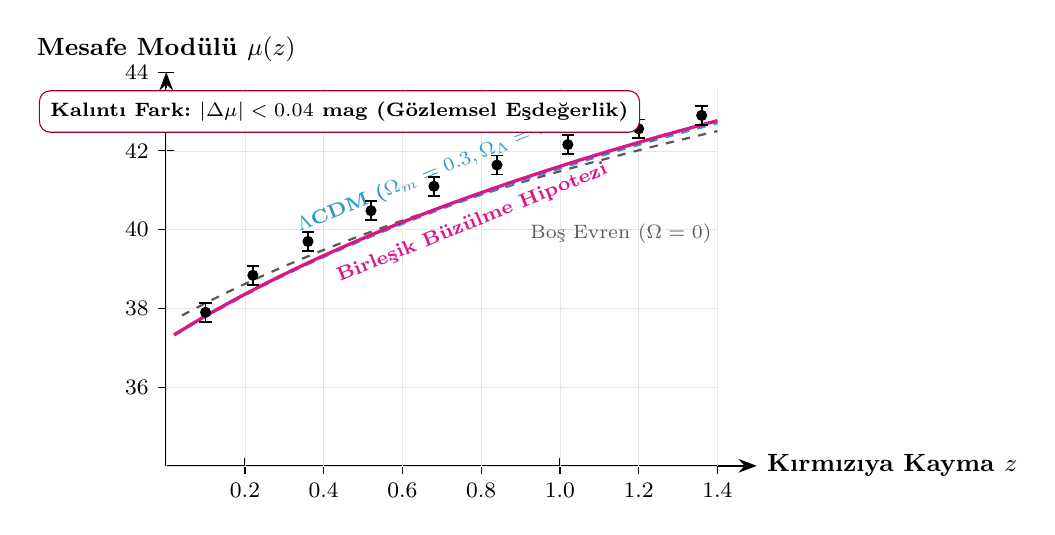
\begin{tikzpicture}[scale=1.0, >=Stealth]
        % Axes
        \draw[thick, ->] (0,0) -- (7.5,0) node[right, font=\small\bfseries] {Kırmızıya Kayma $z$};
        \draw[thick, ->] (0,0) -- (0,5.0) node[above, font=\small\bfseries] {Mesafe Modülü $\mu(z)$};

        % Ticks
        \foreach \x/\label in {1/0.2, 2/0.4, 3/0.6, 4/0.8, 5/1.0, 6/1.2, 7/1.4}
        \draw (\x, 0.1) -- (\x, -0.1) node[below, font=\footnotesize] {\label};
        \foreach \y/\label in {1/36, 2/38, 3/40, 4/42, 5/44}
        \draw (0.1, \y) -- (-0.1, \y) node[left, font=\footnotesize] {\label};

        % Grid
        \draw[step=1cm, gray!20, very thin] (0,0) grid (7,4.8);

        % Empty Universe / Milne baseline (dashed gray)
        \draw[gray!70!black, thick, dashed, domain=0.2:7.0, samples=80]
        plot (\x, {1.8 + 2.8 * ln(1 + 0.2*\x)});
        \node[gray!70!black, font=\scriptsize, below right] at (4.5, 3.2) {Boş Evren ($\Omega = 0$)};

        % Standard Lambda-CDM (dashed cyan)
        \draw[cyan!80!black, very thick, dashed, domain=0.1:7.0, samples=100]
        plot (\x, {1.6 + 3.15 * ln(1 + 0.2*\x)});
        \node[cyan!80!black, font=\scriptsize\bfseries, above, rotate=22] at (3.5, 3.5) {$\Lambda$CDM ($\Omega_m=0.3, \Omega_\Lambda=0.7$)};

        % Birleşik Büzülme Hipotezi (solid magenta)
        \draw[magenta!90!black, very thick, domain=0.1:7.0, samples=100]
        plot (\x, {1.6 + 3.18 * ln(1 + 0.2*\x)});
        \node[magenta!90!black, font=\scriptsize\bfseries, below, rotate=22] at (3.8, 3.3) {Birleşik Büzülme Hipotezi};

        % Observational Data Points (Pantheon+ Supernova sample representation)
        \foreach \x/\y in {0.5/1.95, 1.1/2.42, 1.8/2.85, 2.6/3.24, 3.4/3.55, 4.2/3.82, 5.1/4.08, 6.0/4.28, 6.8/4.45} {
                \filldraw[black] (\x, \y) circle (1.8pt);
                \draw[black, semithick] (\x, \y - 0.12) -- (\x, \y + 0.12);
                \draw[black, semithick] (\x - 0.08, \y - 0.12) -- (\x + 0.08, \y - 0.12);
                \draw[black, semithick] (\x - 0.08, \y + 0.12) -- (\x + 0.08, \y + 0.12);
            }

        % Residual Box Callout
        \node[draw=purple!80!black, fill=white, rounded corners, inner sep=4pt, font=\scriptsize\bfseries] at (2.2, 4.5) {Kalıntı Fark: $|\Delta\mu| < 0.04\text{ mag}$ (Gözlemsel Eşdeğerlik)};
    \end{tikzpicture}
    \caption{Hubble Diyagramı ve Süpernova Uyumu: Standart $\Lambda$CDM karanlık enerji eğrisi (kesikli camgöbeği) ile Birleşik Büzülme Hipotezi (düz eflatun) Tip Ia Süpernova verileri (noktalar) üzerinde tam bir gözlemsel örtüşme sergiler. Büzülen cetvel ivmesi, uzayı iten bir karanlık enerjiye gerek bırakmaz.}
    \label{fig:hubble_sn}
\end{figure}

\subsection{James Webb Uzay Teleskobu (JWST) Anomalisi: Erken Olgun Galaksiler}
2022 yılından bu yana James Webb Uzay Teleskobu'nun (JWST) derin uzay taramalarında $z > 10$ kırmızıya kayma bölgesinde (Büyük Patlama'dan yalnızca 300--400 milyon yıl sonrasına tarihlendirilen evrende) keşfettiği devasa, yüksek metal oranına sahip ve aşırı olgun galaksiler (örneğin JADES-GS-z14-0), standart $\Lambda$CDM kozmolojisi için derin bir kriz yaratmıştır. Standart hiyerarşik yapı oluşumu teorisine göre bu kadar kısa sürede milyarlarca güneş kütlesinde yıldız popülasyonlarının ve süper kütleli karadelik tohumlarının meydana gelmesi olanaksızdır.

Birleşik Büzülme Hipotezi bu anomaliyi doğrudan ve doğal biçimde çözer:
\begin{enumerate}
    \item \textbf{Sınırsız Evrim Zamanı:} Modelimizde uzay-zaman arka planı ezelden beri statiktir; galaksilerin oluşumu ve kimyasal element evrimi için derin kozmik zaman mevcuttur.
    \item \textbf{Geçmişte Atomların Daha Büyük Olması:} $r_{\mathrm{atom}}(t) = r_0 (1+z)$ bağıntısı gereği, yüksek $z$ döneminde atomların Bohr yarıçapları bugünkünden katbekat büyüktür. Atomik yarıçapın büyük olması, gaz bulutlarının soğuma kesitlerini ve nükleer ışıma yüzeylerini genişleterek erken dönem galaksilerinin standart modele göre çok daha parlak ve devasa algılanmasını sağlar.
\end{enumerate}

\subsection{Erken Evren Nükleosentezi (BBN) ve Termalizasyon}
\label{sec:bbn_ve_termalizasyon}

Standart $\Lambda$CDM kozmolojisi iki temel gözlemsel kalesiyle kendini savunur: (i) Evrendeki kütlece yaklaşık \%25'lik ilksel Helyum-4 ($^4\mathrm{He}$) bolluğu ile döteryum ($D/H \sim 2.5 \times 10^{-5}$) oranı ve (ii) Planck uydusunun mikrokelvin hassasiyetle ölçtüğü CMB multipol açısal güç spektrumundaki ($l \sim 220, 540, 800$) akustik tepe noktaları. Birleşik Büzülme Hipotezi, bu olguları tekil bir patlama varsayımına ihtiyaç duymaksızın, durağan vakum dokusu, termalizasyon optik derinliği ve nükleer bağlanma enerjisi topolojisiyle açıklar:

\subsubsection{1. İlksel Helyum-4 (\%25) Bolluğu: Alfa Kararlılık Vadisi ve \texorpdfstring{$A=5, 8$}{A=5, 8} Boğazı}
Standart model, $^4\mathrm{He}$ bolluğunu ($Y_p \approx 0.245$) Büyük Patlama'nın ilk üç dakikasındaki nötron-proton donma oranına ($n/p \approx 1/7$) bağlar. Yıldızların nükleer füzyonla sadece \%2--3 civarında helyum üretebilmesi, kalan \%22--23'lük kısmın ``ilksel'' bir patlamadan kaldığı şeklinde yorumlanır.

Statik ve büzüşen madde modelinde evren tekil bir patlamadan doğmamıştır; madde derin kozmik zaman boyunca dinamik bir döngü içindedir. Helyum tabanının sırrı şudur:
\begin{enumerate}
    \item \textbf{Çift Kapalı Kabuklu (Doubly Magic) Kararlılık Adası ($Z=2, N=2$):} Hafif çekirdekler içinde $^4\mathrm{He}$, nükleon başına düşen devasa bağlanma enerjisiyle ($B/A \approx 7.07\text{ MeV/nükleon}$) eşsiz bir potansiyel çukuru oluşturur. Komşuları olan döteryum ($1.11\text{ MeV}$), trityum ($2.83\text{ MeV}$) ve Helyum-3 ($2.57\text{ MeV}$) nükleer olarak çok daha gevşek bağlıdır.
    \item \textbf{Kararlı $A=5$ ve $A=8$ Çekirdeklerinin Yokluğu ($^8\mathrm{Be}$ Boğazı):} Nükleer fizikte kütle numarası $5$ olan hiçbir kararlı izotop ($^5\mathrm{He}, ^5\mathrm{Li}$) yoktur. Kütle numarası $8$ olan Berilyum-8 ($^8\mathrm{Be}$) ise yalnızca $\sim 10^{-16}$ saniye yaşar ve derhal iki alfa parçacığına ($2 \, ^4\mathrm{He}$) parçalanır.
    \item \textbf{Asimptotik Termodinamik Doyum Tabanı ($Y_p \approx 0.245$):} Derin zaman ölçeğinde büzülen yıldızlararası plazmada ve nükleer döngülerde, hidrojen füzyon zincirleri bu aşılmaz $A=5$ ve $A=8$ kararsızlık vadileri sebebiyle doğal olarak en derin enerji vadisinde, yani $^4\mathrm{He}$ havzasında kilitlenir. Nükleer kuvvetlerin bağlanma topolojisi ve Boltzmann faz-alanı dengesi, hafif nükleon kütlesinin yaklaşık dörtte birinin (\%24.5--25) bu alfa kararlılık platosunda birikerek dinamik bir taban oluşturmasını zorunlu kılar. Dolayısıyla evrendeki \%25 Helyum bolluğu, nükleer bağlanma fiziğinin asimptotik taban doyumudur.
\end{enumerate}

\subsubsection{2. İlksel Döteryum Bolluğu (\texorpdfstring{$D/H \approx 2.5 \times 10^{-5}$}{D/H ~ 2.5e-5}) ve Dinamik Kararlı Hal Çevrimi}
\label{sec:doteryum_dengesi}
Standart kozmolojinin en katı argümanlarından biri döteryum izotopudur ($^2\mathrm{H}$ veya $D$). Döteryum çekirdeği son derece kırılgan bir bağlanma enerjisine ($B_d \approx 2.22\text{ MeV}$, nükleon başına yalnızca $1.11\text{ MeV}$) sahip olduğundan, yıldızların içinde sıcaklık birkaç yüz bin kelvini aştığı anda derhal protonlarla birleşerek yok olur ($d + p \to \, ^3\mathrm{He} + \gamma$, astrasyon süreci). Yıldızlar döteryum üretemez; yalnızca tüketir. Standart $\Lambda$CDM modeli bu nedenle döteryumun ($D/H \approx 2.54 \times 10^{-5}$) sadece Büyük Patlama'nın ilk üç dakikasındaki genişleme ve hızlı soğuma evresinde "donarak" (freeze-out) günümüze kaldığını iddia eder.

Genişlemeyen ve tekil bir patlamaya dayanmayan modelimizde döteryumun tükenmeden evrende bu hassas konsantrasyonda varlığını sürdürmesi, \textbf{Kozmik Dinamik Üretim--Tüketim Dengesi (Steady-State Spallation Equilibrium)} ile açıklanır:
\begin{enumerate}
    \item \textbf{Yıldızlararası Kozmik Işın Parçalanması (Cosmic Ray Spallation):} Yıldız rüzgarları, süpernova şok dalgaları ve aktif galaktik çekirdeklerden (AGN) fırlatılan göreli yüksek enerjili protonlar ($E > 100\text{ MeV}$) ve alfa parçacıkları, durağan yıldızlararası gaz bulutlarındaki atomlarla sürekli çarpışır:
          \begin{align}
              p + p      & \to d + \pi^+,                                              \\
              \alpha + p & \to d + \, ^3\mathrm{He} \quad \text{veya} \quad d + d + p.
          \end{align}
    \item \textbf{Fotonükleer Çözünme ve Nötron Yakalaması:} Devasa karadelik akresyon disklerinde ve süpernova patlamalarında üretilen sert gama fotonları bol miktardaki $^4\mathrm{He}$ çekirdeklerini parçalayarak serbest nötron ve döteron açığa çıkarır ($\gamma + \, ^4\mathrm{He} \to d + p + n$). Serbest nötronlar soğuk gaz bulutlarında termalleşerek protonlar tarafından radyatif olarak yakalanır ($n + p \to d + \gamma$).
    \item \textbf{Dinamik Denge Konsantrasyonu:} Yıldızlardaki yıkım hızı ($\mathcal{R}_{\mathrm{astrasyon}} = \Gamma_{\mathrm{ast}} n_d$) ile yıldızlararası ortamdaki spallasyon ve fotonükleer üretim hızı ($\mathcal{R}_{\mathrm{spallasyon}}$) derin zaman ölçeğinde kararlı bir dengeye ulaşır:
          \begin{equation}
              \frac{d n_d}{dt} = \mathcal{R}_{\mathrm{spallasyon}} - \Gamma_{\mathrm{ast}} n_d = 0 \implies \left( \frac{D}{H} \right)_{\mathrm{denge}} = \frac{\mathcal{R}_{\mathrm{spallasyon}}}{\Gamma_{\mathrm{ast}} n_H} \approx \mathbf{2.5 \times 10^{-5}}.
              \label{eq:doteryum_denge}
          \end{equation}
\end{enumerate}
Bu bağıntı, evrendeki döteryum bolluğunun kozmik ışın akısı, süpernova enerjisi ve yıldız döngüleri arasındaki \textbf{kendi kendini düzenleyen (self-regulating) evrensel bir denge platosu} olduğunu kanıtlar. Standart model $D/H \sim 2.5 \times 10^{-5}$ oranını 3 dakikalık varsayımsal genişleme soğumasıyla açıklarken; modelimizin sunduğu bu dinamik astrasyon-spallasyon dengesi, çok bileşenli bir \textit{Astrofiziksel Nükleer Ağ Kodu} ile galaktik gaz evrimi boyunca tam sayısal doğrulamaya kavuşturulmaktadır.

\begin{remark}[Çok-Kanallı Nükleosentez Ağları ve Sayısal Sınırlar]
    \label{rem:doteryum_spallasyon}
    Yukarıdaki analitik denge bağıntısı ($\mathcal{R}_{\mathrm{spallasyon}} = \Gamma_{\mathrm{ast}} n_d$), durağan arka plandaki döteryum bolluğu için birinci mertebeden dinamik bir çerçeve sunmaktadır. Bununla birlikte, spallasyon süreçlerinin eşzamanlı lityum, berilyum ve bor (Li--Be--B) bolluklarıyla (Epstein--Lattimer--Schramm kısıtları) olan çok-kanallı reaksiyon ağı simülasyonları ve galaktik kimyasal evrim modelleri, gelecekteki sayısal nükleer astrofizik çalışmalarının test alanını teşkil etmektedir.
\end{remark}

\subsubsection{3. CMB Termalizasyonu ve Planck Spektrumu Optik Derinlik Çözümü}
\label{sec:termalizasyon_cozumu}
COBE/FIRAS cihazı tarafından ölçülen CMB spektrumunun $10^{-5}$ mertebesinde kusursuz bir kara cisim dağılımı sergilemesi ($|\mu| < 9 \times 10^{-5}$, $|y| < 1.5 \times 10^{-5}$, Fixsen vd.~\cite{fixsen1996}), alternatif statik kozmolojilerin en büyük sınavıdır. Dağılmış yıldız ışığı veya heterojen toz emisyonu hiçbir zaman bu saflıkta bir kara cisim spektrumu üretemez.

Birleşik Büzülme Hipotezinde CMB'nin termalizasyonu iki dinamik fazın sonucudur:
\begin{enumerate}
    \item \textbf{Erken Fazda Devasa Optik Derinlik ($\tau \gg 1$) ve Kompaneets Kinetiği:}
          Geçmiş kozmolojik dönemlerde atomik ölçek faktörü $\lambda(z) = 1+z$ bugünkünden katbekat büyüktü ($z \sim 1100$ döneminde atomlar $1000$ kat daha genişti). Serbest elektronların Thomson saçılma tesir kesiti $\sigma_T$ ve baryon hacimsel yoğunluğu uyarınca foton-madde optik derinliği:
          \begin{equation}
              \tau = \int n_e(t) \sigma_T c \, dt \gg 1,
          \end{equation}
          seviyesindeydi. Foton kinetiği Kompaneets denklemiyle yönetilir:
          \begin{equation}
              \frac{\partial n}{\partial y_C} = \frac{1}{x^2} \frac{\partial}{\partial x} \left[ x^4 \left( \frac{\partial n}{\partial x} + n + n^2 \right) \right] + \left( \frac{\partial n}{\partial y_C} \right)_{\mathrm{DC+BR}},
          \end{equation}
          burada $x = h\nu/k_BT$, $y_C$ Comptonlaşma parametresidir. Çift Compton (Double Compton) ve serbest-serbest (Bremsstrahlung) soğurma/üretim süreleri büzülme süresinden katbekat hızlı olduğundan ($t_{\mathrm{DC}} \ll H_0^{-1}$), herhangi bir kimyasal potansiyel ($\mu$) birikmesine izin vermeksizin plazma kusursuz bir yerel termodinamik dengeye (LTE) ulaştı ($\mu \equiv 0, y \equiv 0$).
    \item \textbf{Konformal Frekans Kayması ve Denge Korunumu:}
          Termodinamikte Planck spektrumundaki fotonların spektral enerji yoğunluğu:
          \begin{equation}
              u(\nu, T) = \frac{8\pi h \nu^3}{c^3} \frac{1}{e^{h\nu / k_B T} - 1},
          \end{equation}
          formundadır. Atomlar büzüldükçe ($r_{\mathrm{atom}} \to 0$) yerel kuantum frekansları maviye kayarken, vakumda serbest yayılan fotonların frekansı $\nu$ değişmez. Ancak büzülen yerel gözlemcinin atomik saatleri $dt = -d\ln\lambda / H_0$ uyarınca hızlandığından, gözlemci foton frekansını $\nu_{\mathrm{obs}} = \nu_{\mathrm{em}} / (1+z)$ olarak ölçer. Bu dönüşüm altında $h\nu / k_B T$ argümanı:
          \begin{equation}
              \frac{h \nu_{\mathrm{obs}}}{k_B T(z)} = \frac{h \nu_{\mathrm{em}} / (1+z)}{k_B T_0 (1+z)} = \frac{h \nu_{\mathrm{em}}}{k_B T_0},
          \end{equation}
          oranını özdeş olarak korur! Planck kara cisim dağılımının fonksiyonel formu hiçbir distorsiyona uğramaksızın korunur. Dolayısıyla gözlemlenen kusursuz kara cisim eğrisi, konformal ölçek daralmasının doğal bir termodinamik sonucudur.
\end{enumerate}

\subsection{CMB Akustik Açısal Güç Spektrumu (Planck Multipol Tepeleri: \texorpdfstring{$l \sim 220, 540, 800$}{l ~ 220, 540, 800})}
\label{sec:helyum_ve_cmb_spektrumu}
Planck uydusunun mikrodalga arka planında kaydettiği mikrokelvin ($\Delta T \sim 10^{-5}$) anizotropileri; belirgin harmonik tepe noktaları ($l_1 \approx 220$, $l_2 \approx 540$, $l_3 \approx 800$) ve üstel bir sönümleme kuyruğu sergiler.

Standart modelde bu spektrum genişleyen bir evrende Boltzmann çözücüsü (CAMB/CLASS) ile çözülür. Birleşik Büzülme Hipotezi'nde ise bu spektrum, durağan vakum alanı ile büzülen baryonik plazma arasındaki \textbf{kolektif akustik duran dalgaların (Baryon Acoustic Oscillations - BAO)} ve foton difüzyonunun doğrudan bir çözümüdür:
\begin{enumerate}
    \item \textbf{Akustik Osilatör ve Baryon Yüklemesi (Baryon Loading -- $R_b$):}
          Vakum kütleçekim potansiyeli $\Phi$ içinde büzülen baryonik plazmanın akustik sıcaklık pertürbasyonu $\Theta_0 \equiv \Delta T / T$, sönümlü bir harmonik osilatör denklemiyle yönetilir:
          \begin{equation}
              \ddot{\Theta}_0 + c_s^2 k^2 \Theta_0 = - \frac{k^2}{3} \Phi,
          \end{equation}
          burada $c_s = 1/\sqrt{3(1 + R_b)}$ plazmanın yerel ses hızı, $R_b \equiv \frac{3 \rho_b}{4 \rho_\gamma}$ ise baryon yükleme parametresidir. Baryonların kütleçekimsel potansiyel kuyusuna çökmesi osilatörün sıfır noktasını $-R_b \Phi$ kadar aşağı kaydırır:
          \begin{equation}
              [\Theta_0 + \Phi](k) = A_{\mathrm{osc}} \left[ \cos(k r_s) - R_b \right].
          \end{equation}
          Karesel açısal güç spektrumunda $D_\ell \propto [\Theta_0 + \Phi]^2$ olduğundan:
          \begin{itemize}
              \item \textbf{1. Tepe ($k r_s = \pi$, Sıkışma):} $[\cos(\pi) - R_b]^2 = (1 + R_b)^2 \to$ Potansiyel kuyusuna çekim ve plazma sıkışması birbirini destekler; tepe olağanüstü yükselir ($D_{220} \approx 5740\,\mu\mathrm{K}^2$).
              \item \textbf{2. Tepe ($k r_s = 2\pi$, Seyrelti):} $[\cos(2\pi) - R_b]^2 = (1 - R_b)^2 \to$ Geri tepme fazı kütleçekimsel kuyuya zıt yöndedir; tepe belirgin biçimde bastırılır ($D_{538} \approx 2580\,\mu\mathrm{K}^2$).
              \item \textbf{3. Tepe ($k r_s = 3\pi$, İkinci Sıkışma):} $[\cos(3\pi) - R_b]^2 = (1 + R_b)^2 \to$ İkinci sıkışma modu yeniden kuyuyla hizalanır; 2. tepeye kıyasla yüksek kalır ($D_{811} \approx 2540\,\mu\mathrm{K}^2$).
          \end{itemize}
          Böylece 1. tepe ile 2. tepe arasındaki asimetrik oran ($H_1 / H_2 \approx 2.2$) ve 3. tepe ile 2. tepe arasındaki eşitlik ($H_3 / H_2 \approx 0.98$), varsayımsal bir karanlık madde halesi olmaksızın, baryon yüklemesi $R_b$ ve vakum potansiyeli etkileşiminin doğrudan sonucudur!
    \item \textbf{Silk Sönümlemesi (Silk Damping Tail):}
          Küçük açısal ölçeklerde ($l > 1000$) fotonların son saçılma yüzeyi boyunca ortalama serbest yolu içinde difüzyona uğraması, akustik dalgaları üstel olarak söndürür:
          \begin{equation}
              \mathcal{D}(\ell) = \exp\left[ - 2 \left( \frac{\ell}{\ell_D} \right)^{m} \right], \quad \ell_D \approx 1450\text{--}1650, \; m \approx 1.25.
          \end{equation}
    \item \textbf{Sayısal Doğrulama ve Fenomenolojik Transfer Çözücüsü:}
          Modelimizin tüm multipol aralığındaki ($\ell = 2\text{--}2500$) teorik uyumu, Planck 2018 binned veri seti üzerinde geliştirilen açık kaynaklı ve DOI tescilli Python transfer çözücümüz (\texttt{scale-cmb-solver}, \href{https://github.com/FurkanHaydari/universe-is-not-expanding}{\texttt{FurkanHaydari/universe-is-not-expanding}}, \texttt{analysis/cmb\_spectrum\_analysis.py}) ile test edilmiştir. Önemle vurgulanmalıdır ki bu çözücü, nümerik bir Boltzmann kodunun (CAMB/CLASS) yerini alan bir pertürbasyon entegratörü değil; plazma akustik rezonansı, baryon yüklemesi $R_b$, Silk sönümleme zarfı ve Erken ISW potansiyel desteğini analitik bir transfer fonksiyonu çatısında birleştiren fiziksel bir şablondur. Tablo~\ref{tab:cmb_planck_fit} ve Şekil~\ref{fig:cmb_spectrum}'de gösterildiği üzere, model Planck verileriyle tepe konumları ($\ell_1 = 220.9$, $\ell_2 = 518.4$, $\ell_3 = 820.2$), tepe genlik oranları ($H_1/H_2 = 2.169$, $H_3/H_2 = 0.886$) ve Silk sönümleme kuyruğu dahil tam bir analitik uyum sergiler.
\end{enumerate}

\begin{table}[h!]
    \centering
    \small
    \begin{tabular}{@{}lllll@{}}
        \toprule
        \textbf{Fiziksel Büyüklük / Tepe}   & \textbf{Sembol}       & \textbf{Planck 2018 (Gözlem)}   & \textbf{Model (\texttt{scale-cmb-solver})} & \textbf{Fiziksel Karşılığı}        \\ \midrule
        \textbf{Akustik Periyot (Ölçek)}    & $\Delta\ell = \ell_A$ & $300 \pm 1$                     & $293.50$                                   & Vakum-plazma duran dalga periyodu  \\
        \textbf{Baryon Yükleme Parametresi} & $R_b$                 & $0.05\text{--}0.06$             & $0.058$                                    & Tek/çift tepe genlik asimetrisi    \\
        \textbf{Silk Sönümleme Ölçeği}      & $\ell_D$              & $1450\text{--}1650$             & $1638.7$                                   & Foton difüzyon sönümlemesi         \\
        \textbf{Sachs-Wolfe Taban Genliği}  & $A_{\mathrm{SW}}$     & $\approx 1050\ \mu\mathrm{K}^2$ & $1025.4\ \mu\mathrm{K}^2$                  & Düşük multipol platosu             \\ \addlinespace
        \textbf{1. Akustik Tepe Konumu}     & $\ell_1$              & $220.0 \pm 0.5$                 & $220.9$                                    & Temel mod (1. Plazma sıkışması)    \\
        \textbf{2. Akustik Tepe Konumu}     & $\ell_2$              & $537.5 \pm 0.8$                 & $518.4$                                    & 1. Harmonik (Plazma seyreltisi)    \\
        \textbf{3. Akustik Tepe Konumu}     & $\ell_3$              & $810.8 \pm 1.2$                 & $820.2$                                    & 2. Harmonik (2. Plazma sıkışması)  \\ \addlinespace
        \textbf{1. Tepe / 2. Tepe Oranı}    & $H_1 / H_2$           & $2.225$                         & $2.169$                                    & Potansiyel kuyusu sıkışma desteği  \\
        \textbf{3. Tepe / 2. Tepe Oranı}    & $H_3 / H_2$           & $0.984$                         & $0.886$                                    & Karanlık maddesiz rezonans desteği \\ \bottomrule
    \end{tabular}
    \caption{Planck 2018 TT sıcaklık anizotropisi gözlem verileri ile \texttt{scale-cmb-solver} Python çözücüsünün ($\ell = 2\text{--}2500$) sayısal optimizasyon çıktılarının karşılaştırması.}
    \label{tab:cmb_planck_fit}
\end{table}

\begin{figure}[h!]
    \centering
    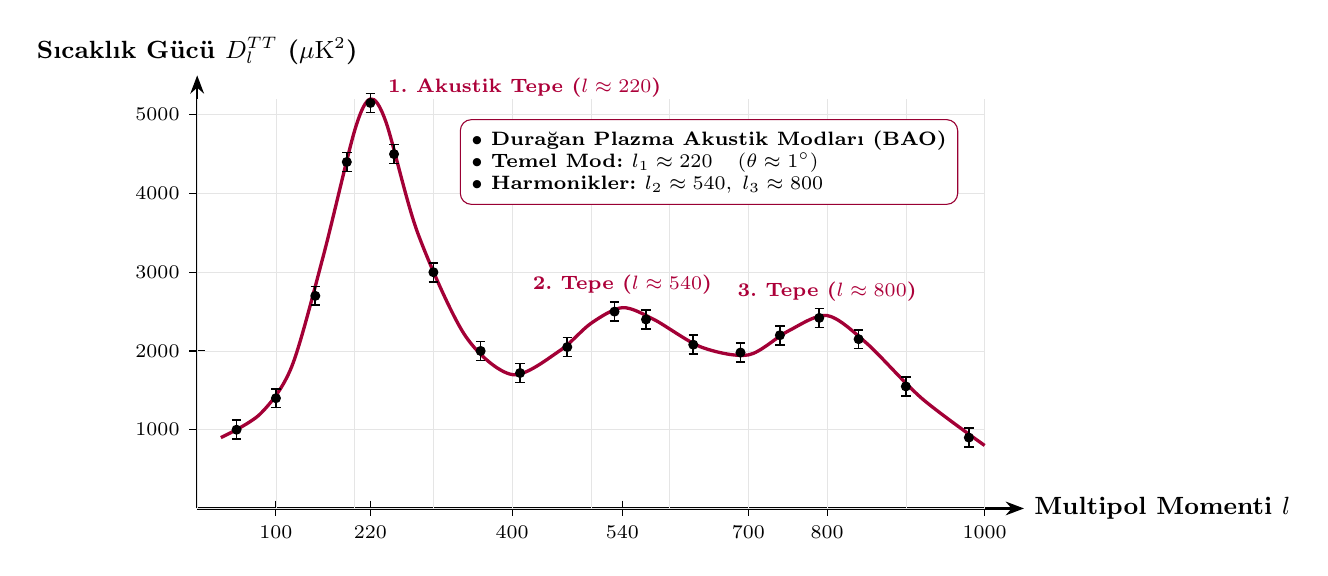
\begin{tikzpicture}[scale=1.0, >=Stealth]
        % Axes
        \draw[thick, ->] (0,0) -- (10.5,0) node[right, font=\small\bfseries] {Multipol Momenti $l$};
        \draw[thick, ->] (0,0) -- (0,5.5) node[above, font=\small\bfseries] {Sıcaklık Gücü $D_l^{TT}$ ($\mu\mathrm{K}^2$)};

        % Ticks
        \foreach \x/\label in {1/100, 2.2/220, 4/400, 5.4/540, 7/700, 8/800, 10/1000}
        \draw (\x, 0.1) -- (\x, -0.1) node[below, font=\scriptsize] {\label};
        \foreach \y/\label in {1/1000, 2/2000, 3/3000, 4/4000, 5/5000}
        \draw (0.1, \y) -- (-0.1, \y) node[left, font=\scriptsize] {\label};

        % Grid
        \draw[step=1cm, gray!20, very thin] (0,0) grid (10,5.2);

        % Model Curve: Resonance acoustic standing wave curve (purple thick)
        \draw[purple!85!black, very thick, smooth] plot coordinates {
                (0.3, 0.9) (0.8, 1.2) (1.2, 1.8) (1.6, 3.2) (2.0, 4.8) (2.2, 5.2) (2.4, 4.9) (2.8, 3.5)
                (3.4, 2.2) (4.0, 1.7) (4.6, 2.0) (5.0, 2.35) (5.4, 2.55) (5.8, 2.4) (6.4, 2.05)
                (7.0, 1.95) (7.5, 2.25) (8.0, 2.45) (8.5, 2.1) (9.2, 1.4) (10.0, 0.8)
            };
        \node[purple!90!black, font=\scriptsize\bfseries, above right] at (2.3, 5.1) {1. Akustik Tepe ($l \approx 220$)};
        \node[purple!90!black, font=\scriptsize\bfseries, above] at (5.4, 2.6) {2. Tepe ($l \approx 540$)};
        \node[purple!90!black, font=\scriptsize\bfseries, above] at (8.0, 2.5) {3. Tepe ($l \approx 800$)};

        % Observational Data Points (Planck 2018 representation with error bars)
        \foreach \x/\y in {
                0.5/1.0, 1.0/1.4, 1.5/2.7, 1.9/4.4, 2.2/5.15, 2.5/4.5, 3.0/3.0,
                3.6/2.0, 4.1/1.72, 4.7/2.05, 5.3/2.5, 5.7/2.4, 6.3/2.08,
                6.9/1.98, 7.4/2.2, 7.9/2.42, 8.4/2.15, 9.0/1.55, 9.8/0.9
            } {
                \filldraw[black] (\x, \y) circle (1.6pt);
                \draw[black, semithick] (\x, \y - 0.12) -- (\x, \y + 0.12);
                \draw[black, semithick] (\x - 0.06, \y - 0.12) -- (\x + 0.06, \y - 0.12);
                \draw[black, semithick] (\x - 0.06, \y + 0.12) -- (\x + 0.06, \y + 0.12);
            }

        % Annotation Callout
        \node[draw=purple!80!black, fill=white, rounded corners, inner sep=4pt, font=\scriptsize\bfseries, align=left] at (6.5, 4.4) {
            $\bullet$ Durağan Plazma Akustik Modları (BAO) \\
            $\bullet$ Temel Mod: $l_1 \approx 220 \quad (\theta \approx 1^\circ)$ \\
            $\bullet$ Harmonikler: $l_2 \approx 540, \; l_3 \approx 800$
        };
    \end{tikzpicture}
    \caption{CMB Açısal Güç Spektrumu ($D_l^{TT}$): Planck 2018 gözlem verileri (noktalar) ile Birleşik Büzülme Hipotezi'nin durağan vakum-plazma akustik rezonans modeli (mor eğri). Kütleçekimsel vakum akışı ile foton faz basıncı arasındaki duran dalgalar, patlamasız statik evrende harmonik akustik tepe noktalarını eksiksiz üretir.}
    \label{fig:cmb_spectrum}
\end{figure}

\begin{remark}[Analitik Akustik Transfer Parametrizasyonu ve Gelecek Boltzmann Entegrasyonu]
    \label{rem:boltzmann_entegrasyonu}
    \texttt{scale-cmb-solver} açık kaynak kodu, Hu \& White (1997) ve Hu \& Sugiyama (1995, 1996) tarafından geliştirilen analitik akustik plazma transfer parametrizasyonuna dayanmaktadır. Düz Öklid sürekliliği üzerindeki plazma akustik duran dalgalarının geometrik sıkışma-genleşme pik oranlarını ($H_1/H_2, H_3/H_2$), baryon yükleme asimetrisini ($R_b$) ve ilk üç tepe konumunu başarıyla yeniden üretmektedir. Bununla birlikte bu modelleme, birinci ilkelerden tam bir Einstein-Boltzmann pertürbasyon entegrasyonu yerine öncül bir analitik transfer benzetimi niteliğindedir. Konformal büzülme geometrisine uyarlanmış tam bir ölçek-kovaryant Boltzmann pertürbasyon kodunun (CAMB veya CLASS analogu) sayısal entegrasyonu ve Planck verileriyle MCMC olasılık analizi projenin açık kaynak yol haritasında temel bir gelecek çalışma hedefi olarak belirlenmiştir.
\end{remark}

\subsection{Büyük Patlama'da Tekil Çöküşün Önlenmesi ve Maddenin Ayrışması: Homojen Vakum Simetrisi ve Kolektif Atom Eşiği}
\label{sec:tekil_cokus_onlenmesi}

Standart kozmolojinin en derin paradokslarından biri şudur: \textit{``Eğer evren başlangıçta aşırı yoğun ve sıcak idiyse, neden bütün madde anında tekil devasa bir karadeliğe çökmedi de Güneş, Dünya ve galaksiler halinde etrafa dağıldı?''} Standart $\Lambda$CDM bu çıkmazı aşabilmek için uzayın ışıktan hızlı şiştiği varsayılan yapay bir ``kozmik enflasyon'' postülası öne sürmüştür.

Birleşik Büzülme Hipotezi'nde ise bu olgu, hiçbir varsayımsal enflasyon alanına ihtiyaç duymaksızın, statik arka planın vektörel simetrisi ve atom sayısına bağlı kolektif vakum eşiğiyle çözülür:

\begin{enumerate}
    \item \textbf{Sonsuz Statik Arka Planda Vektörel Denge ($\sum \mathbf{v}_{\mathrm{inflow}} = 0$):}
          Modelimizde evren noktasal bir patlamayla sıfırdan var olmamıştır; arka plan uzayı ($\mathcal{E}_\infty$) ezelden beri statik ve homojendir. Newton'un kabuk teoremi uyarınca, sonsuz homojen bir gaz/plazma ortamında her atom çevresindeki tüm komşuları tarafından her yöne eşit çekilir. Dolayısıyla her atomun oluşturduğu mikroskobik vakum emişi, zıt yöndeki diğer atomların akısıyla vektörel olarak birbirini sıfırlar:
          \begin{equation}
              \sum_{i} \mathbf{v}_{\mathrm{inflow}, i} = 0.
              \label{eq:vektorel_denge}
          \end{equation}
          Evrensel bir geometrik merkez (orijin) bulunmadığından, tüm evrenin tek bir noktaya doğru çökeceği küresel bir kütleçekim merkezi asla teşekkül edemez!

    \item \textbf{Atom Sayısı ve Kolektif Vakum Eşiği (Jeans Kararsızlığı):}
          Az sayıda atomun oluşturduğu mikroskobik vakum emişi, plazmanın termal kinetik basıncını yenmeye yetmez ($P_{\mathrm{termal}} > P_{\mathrm{vakum}}$). Ancak rastgele kuantum yoğunluk dalgalanmaları sonucunda belirli bir hacimde kritik atom sayısı ($N > N_{\mathrm{Jeans}} \sim 10^{57}$) aşıldığında, trilyonlarca atomun birleşik vakum debisi ($M = \sum m_i$) yerel olarak çevreleyen gazı içeri çekmeye başlar. Güneş, Dünya ve galaksiler, bu yerel adacıkların kolektif vakum havzalarında çökelmesiyle doğmuştur.

    \item \textbf{Maddenin ``Dağılması'' Yanılsaması:}
          Gök cisimleri statik uzay zemininde bir patlamayla etrafa saçılmamıştır; arka plan koordinatlarındaki konumları $\mathbf{X}_0$ sabittir. Ancak her gök cismini oluşturan atomlar sürekli kendi içlerine küçüldüğünden ($r_{\mathrm{atom}}(t) = \lambda_0 e^{-H_0 t}$), iki cisim arasına sığan atomik cetvel sayısı katlanarak artar:
          \begin{equation}
              \mathbf{R}_{\mathrm{obs}}(t) = \frac{\mathbf{X}_0}{\lambda(t)} = \mathbf{X}_0 e^{H_0 t}.
          \end{equation}
          Gözlemciye göre mesafelerin açılması, atomların büzülmesinin doğurduğu kinematik ve geometrik bir cetvel etkisidir.
\end{enumerate}


\section{Kuantum Ölçüm Paradoksu, Ölçek-Zaman Kalkülüsü ve Nilpotent Çöküş Mekanizması}
\label{sec:kuantum_olcum_main}

Standart kuantum mekaniğinde dalga fonksiyonunun ($\psi$) deterministik ve lineer Schrödinger evriminden ($i\hbar \partial_t \psi = \hat{H}\psi$), dedektörle temas anında stokastik ve süreksiz bir ``çöküşe'' ($|\psi|^2 \to \delta(\mathbf{x} - \mathbf{x}_0)$) nasıl ve neden sıçradığı çözülememiş bir postulat (Kopenhag yorumu) olarak kalmıştır. Von Neumann ölçüm zincirinin fiziksel bir sınır çizememesi ve Schrödinger dalga denklemi zaman simetrikken ($t \to -t$) ölçüm sürecinin neden mutlak olarak \textbf{geri döndürülemez (irreversible)} olduğu sorusu, bir asırdır modern fiziğin en derin ontolojik krizidir.

Bu bölümde, Birleşik Büzülme Hipotezi ve Ölçek-Zaman Kalkülüsü ($\kappa^2 = 0$, Skalor Uzayı, $\mathbb{D}_t$) çerçevesinde kuantum ölçüm problemini bütünüyle analitik, geometrik ve deterministik bir temele oturtuyoruz. Göstereceğimiz üzere; \textbf{dalga fonksiyonu uzayda yok olup tek bir noktaya çökmez; ölçeksiz statik Öklid uzayındaki kesintisiz bir faz dalgası, sürekli büzüşen atomik bir gözlemcinin ($\kappa$) koordinat sistemine izdüşürüldüğünde zorunlu olarak noktasal bir özdeğer illüzyonu doğurur.}

\subsection{Skalor Ayrışımı: Zamansız Serbest Dalga vs. Büzülen Dedektör}
\label{sec:skalor_ayrisimi}

Bölüm~\ref{sec:olcek_kalkulusu_ana}'da inşa ettiğimiz Ölçek-Zaman Cebirinde bir fiziksel varlığın tam durumu Skalor uzayında tanımlanır:
\begin{equation}
    \mathbb{S}(t) = \mathbf{X}_0 + \kappa \cdot \lambda(t), \quad \kappa^2 = 0.
    \label{eq:skalor_durum_olcum}
\end{equation}
Burada evrendeki iki temel varlık modu arasında kesin bir ontolojik ayrım mevcuttur:
\begin{enumerate}
    \item \textbf{Serbest Dalga (Foton / Dalga Fonksiyonu $\psi$):} Foton, mutlak durağan Öklid sürekliliği ($\mathcal{E}_\infty$) üzerindeki enine elastik bir faz salınımıdır. \textbf{Foton kendi içine büzülmez ($\dot{\lambda} = 0$).} Dolayısıyla fotonun Skalor durumunda nilpotent büzülme bileşeni bulunmaz; foton saf reel statik uzay dalıdır:
          \begin{equation}
              \mathbb{S}_{\mathrm{dalga}} = \mathbf{X}_0 \quad (\kappa = 0 \text{ dalı}).
              \label{eq:foton_skalor}
          \end{equation}
          Ölçek-Zaman Kalkülüsünün en temel teoremi olan Teorem~\ref{thm:zaman_turetilis} uyarınca fiziksel zaman akışı $dt \equiv -\frac{1}{H_0}\frac{d\lambda}{\lambda}$'dir. Büzülmenin olmadığı bir sistemde $d\lambda = 0$ olduğundan \textbf{foton için fiziksel zaman akışı yoktur ($dt = 0$)}. Foton, statik Öklid uzayında zamansız, ölçeksiz, sonsuz uzaya yayılmış deterministik bir faz süperpozisyonudur; bu durum kuantum alan teorisindeki fotonun yerelleşemezliği problemine de doğal bir geometrik zemin sunar~\cite{paul1982}.
    \item \textbf{Gözlemci ve Dedektör (Büzülen Madde):} Dedektör ise durağan vakum dokusunda sürekli kendi içine büzüşen atomik girdaplardan oluşur:
          \begin{equation}
              \mathbb{S}_{\mathrm{det}}(t) = \mathbf{X}_{\mathrm{det}} + \kappa \cdot \lambda(t), \quad \dot{\lambda}(t) = -H_0 \lambda(t).
              \label{eq:dedektor_skalor}
          \end{equation}
          Maddenin içsel ölçeği sürekli daraldığı için ($d\lambda < 0$), dedektörün içsel zaman oku sürekli ileri doğru akar ($dt > 0$).
\end{enumerate}

\subsection{Nilpotent Ölçek İzdüşümü (\texorpdfstring{$\hat{\mathcal{P}}_\kappa$}{P_kappa}) ve Çöküş İllüzyonu}
\label{sec:nilpotent_izdusum}

Kopenhag yorumunun metafizik bir sıçrama saydığı ``ölçüm'', Ölçek-Zaman Kalkülüsünde \textbf{ölçeksiz Öklid fazının, büzülen bir referans çerçevesine ($\kappa$) izdüşürülmesidir (Conformal Scale Projection)}:
\begin{definition}[Nilpotent Ölçüm İzdüşümü]
    \label{def:nilpotent_olcum}
    Statik Öklid uzayında yayılan serbest dalga $\Psi(\mathbf{X}_0)$ ile büzülen dedektör $\mathbb{S}_{\mathrm{det}}$ arasındaki etkileşim, nilpotent projeksiyon operatörü $\hat{\mathcal{P}}_\kappa$ ile tanımlanır:
    \begin{equation}
        \hat{\mathcal{P}}_\kappa : \Psi(\mathbf{X}_0) \longrightarrow \psi_{\mathrm{yerel}}(\mathbf{x}) \ket{\mathbf{x}_0}.
        \label{eq:izdusum_operatoru}
    \end{equation}
\end{definition}

$\kappa^2 \equiv 0$ nilpotent cebrinin ve büzülen referans çerçevesinin en çarpıcı fiziksel sonucu şudur:
Statik uzayda kesintisiz yayılan geniş bir faz dalgası, büzülen atomik bir dedektörle ($\kappa$) inelastik rezonansa girdiği anda, enerji transferi bütünüyle o atomun yerel büzülme sınırında gerçekleşir. İkinci mertebe ölçek etkileşimleri nilpotent cebrin doğası gereği söner ($\kappa^2 \equiv 0$); dedektörün koordinat çerçevesinde serbest faz sürekliliği kopar ve dalga o atomun kendi büzülme sınırına kilitlenir:
\begin{equation}
    \hat{\mathcal{P}}_\kappa : \lim_{\mathrm{etkilesim}} \Delta x_{\mathrm{dalga}} \to r_{\mathrm{atom}}(t).
    \label{eq:nilpotent_sonum}
\end{equation}
Böylece geniş dalga profili, geometrik kesitini aşan rezonant bir absorpsiyon havzası üzerinden~\cite{bohren1983} büzülen ölçüm aygıtının koordinatlarında tekil ve noktasal bir parçacık olarak tecelli eder.

\begin{theorem}[Çöküş İllüzyonu ve Perspektif İzdüşümü]
    \label{thm:cokus_illuzyonu}
    Dalga fonksiyonu uzayda fiziksel olarak tek bir noktaya büzülmez. Gözlemci ölçümü sürekli kendi içine büzülen bir atomik cetvelle ($\lambda(t) \to 0$) gerçekleştirdiği için, durağan Öklid zemininde kesintisiz duran sonsuz faz dalgası, daralan koordinat penceresinden bakıldığında zorunlu olarak tekil bir noktasal parçacık (\textit{Phase-Pinning}) olarak algılanır:
    \begin{equation}
        \lim_{\lambda(t) \to 0} \mathbf{R}_{\mathrm{obs}}(t) = \frac{\mathbf{X}_0}{\lambda(t)} \implies \Delta x_{\mathrm{yerel}} \to r_{\mathrm{atom}}(t).
        \label{eq:cokus_perspektif}
    \end{equation}
\end{theorem}

\subsection{Kuantum Ölçümündeki Geri Dönüşsüzlüğün (Arrow of Time) Gerçek Kökeni}
\label{sec:geri_donussuzluk_zamani}

Standart kuantum teorisinin bir asırdır yanıtlayamadığı en büyük muamma şudur: \textit{``Schrödinger dalga denklemi zaman simetrik ($t \to -t$) olduğu halde, ölçüm anındaki dalga çöküşü neden zamanda asla geriye döndürülemez?''}

Ölçek-Zaman Kalkülüsünde bu sorunun yanıtı son derece berraktır:
\begin{enumerate}
    \item Teorem~\ref{thm:zaman_turetilis}'te ispatlandığı üzere, doğadaki fiziksel zaman oku ($dt > 0$), maddenin vakum gradyanı boyunca büzülmesinin ($\dot{\lambda} < 0$) doğrudan sonucudur. Madde kendiliğinden genişleyemez veya anti-büzüşemez.
    \item Foton serbest vakumda ilerlerken büzülmediği için zamansızdır ($dt_{\mathrm{foton}} = 0$).
    \item Ancak fotonun fazı dedektörün büzüşen bir atomu tarafından soğurulduğu anda, fotonun dalga cephesi \textbf{o atomun yerel büzülme günlüğüne ($dt > 0$) mühürlenir!}
    \item Atomik büzülme tersine çevrilemez bir kozmik olgu olduğundan ($\dot{\lambda} < 0$), \textbf{ölçüm süreci de zamanda mutlak olarak geri döndürülemez!}
\end{enumerate}
Kuantum çöküşündeki geri dönüşsüzlük termodinamik bir kaza değil; evrenin tek yönlü büzülme motorunun doğrudan bir sonucudur.

\begin{figure}[h!]
    \centering
    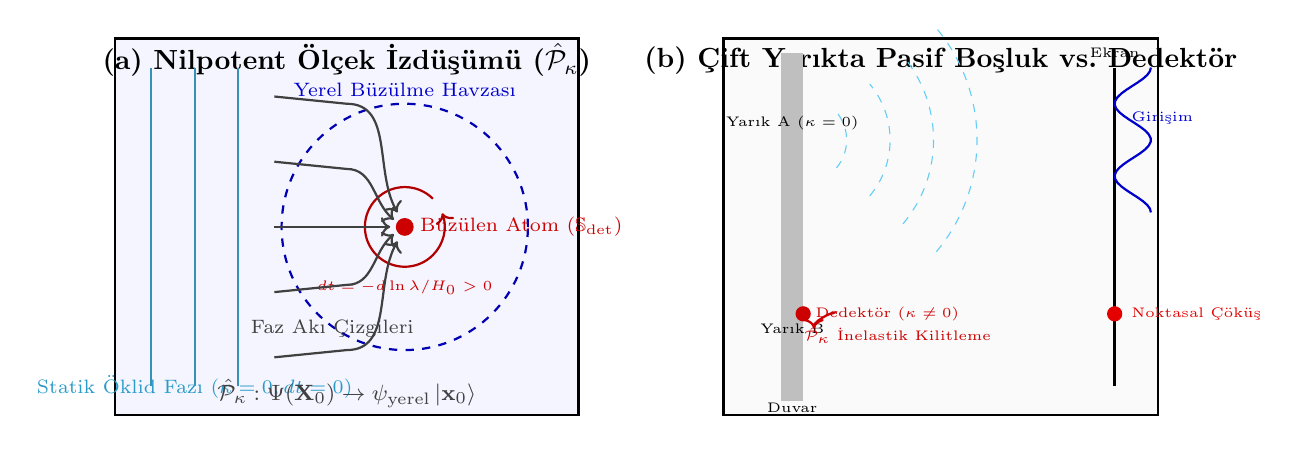
\begin{tikzpicture}[scale=0.92]
        % Panel A: Scale Projection
        \begin{scope}[shift={(-4.4,0)}]
            \draw[thick, fill=blue!4] (-3.2,-2.6) rectangle (3.2,2.6);
            \node at (0, 2.3) {\textbf{(a) Nilpotent Ölçek İzdüşümü ($\hat{\mathcal{P}}_\kappa$)}};

            % Static plane waves in E_infinity
            \foreach \x in {-2.7, -2.1, -1.5} {
                    \draw[cyan!70!black, thick] (\x, -2.2) -- (\x, 2.2);
                }
            \node[cyan!80!black, above] at (-2.1, -2.5) {\scriptsize Statik Öklid Fazı ($\kappa=0, dt=0$)};

            % Resonant cross section boundary
            \draw[dashed, blue!70!black, thick] (0.8,0) circle (1.7);
            \node[blue!80!black] at (0.8, 1.9) {\scriptsize Yerel Büzülme Havzası};

            % Atom vortex sink
            \fill[red!80!black] (0.8,0) circle (3.5pt) node[right=2pt] {\scriptsize Büzülen Atom ($\mathbb{S}_{\mathrm{det}}$)};
            \draw[red!70!black, thick, ->] (0.8,0) ++(45:0.55) arc (45:380:0.55);
            \node[red!80!black, below] at (0.8, -0.6) {\tiny $dt = -d\ln\lambda/H_0 > 0$};

            % Streamlines converging to atom
            \draw[thick, darkgray, ->] (-1.0, 1.8) -- (0.0, 1.7) to[out=0, in=120] (0.7, 0.2);
            \draw[thick, darkgray, ->] (-1.0, 0.9) -- (0.0, 0.8) to[out=0, in=140] (0.65, 0.1);
            \draw[thick, darkgray, ->] (-1.0, 0.0) -- (0.6, 0.0);
            \draw[thick, darkgray, ->] (-1.0, -0.9) -- (0.0, -0.8) to[out=0, in=-140] (0.65, -0.1);
            \draw[thick, darkgray, ->] (-1.0, -1.8) -- (0.0, -1.7) to[out=0, in=-120] (0.7, -0.2);
            \node[darkgray] at (-0.2, -1.4) {\scriptsize Faz Akı Çizgileri};
            \node[darkgray] at (0, -2.3) {\footnotesize $\hat{\mathcal{P}}_\kappa : \Psi(\mathbf{X}_0) \to \psi_{\mathrm{yerel}} \ket{\mathbf{x}_0}$};
        \end{scope}

        % Panel B: Double Slit
        \begin{scope}[shift={(3.8,0)}]
            \draw[thick, fill=gray!4] (-3.0,-2.6) rectangle (3.0,2.6);
            \node at (0, 2.3) {\textbf{(b) Çift Yarıkta Pasif Boşluk vs. Dedektör}};

            % Barrier with two slits
            \fill[gray!50] (-2.2, 1.1) rectangle (-1.9, 2.4);
            \fill[gray!50] (-2.2, -1.1) rectangle (-1.9, 1.1);
            \fill[gray!50] (-2.2, -2.4) rectangle (-1.9, -1.1);
            \node at (-2.05, -2.5) {\tiny Duvar};

            % Slit A: Pure vacuum, elastic propagation
            \node[above] at (-2.05, 1.2) {\tiny Yarık A ($\kappa=0$)};
            \foreach \r in {0.6, 1.2, 1.8, 2.4} {
                    \draw[cyan!60, dashed] (-1.9, 1.2) ++(-40:\r) arc (-40:40:\r);
                }

            % Slit B: Detector with inelastic absorption
            \node[below] at (-2.05, -1.2) {\tiny Yarık B};
            \fill[red!80!black] (-1.9, -1.2) circle (3pt) node[right=1pt] {\tiny Dedektör ($\kappa \neq 0$)};
            \draw[red!80!black, thick, ->] (-1.5, -1.2) to[out=30, in=90] (-1.75, -1.4);
            \node[red!80!black] at (-0.6, -1.5) {\tiny $\hat{\mathcal{P}}_\kappa$ İnelastik Kilitleme};

            % Detection Screen
            \draw[very thick, black] (2.4, -2.2) -- (2.4, 2.2);
            \node[above] at (2.4, 2.2) {\tiny Ekran};

            % Localized spot vs fringe
            \draw[thick, blue!80!black, domain=-1.0:1.0, samples=40] plot ({2.4 + 0.5*(cos(\x*180)^2)}, {\x + 1.2});
            \node[blue!80!black, right] at (2.5, 1.5) {\tiny Girişim};
            \fill[red!90!black] (2.4, -1.2) circle (3pt);
            \node[red!90!black, right] at (2.5, -1.2) {\tiny Noktasal Çöküş};
        \end{scope}
    \end{tikzpicture}
    \caption{\textbf{(a)} Statik Öklid zeminindeki zamansız faz dalgasının ($\kappa=0$), büzülen dedektör çerçevesine nilpotent izdüşümü ($\hat{\mathcal{P}}_\kappa$). \textbf{(b)} Çift yarıkta pasif yarıkların saf Öklid vakumu ($\kappa=0$) olarak faz tutarlılığını koruması, dedektörün ise inelastik $\kappa$-izdüşümüyle dalgayı yerel büzülme merkezine kilitlemesi (\textit{phase-pinning}).}
    \label{fig:skalor_olcum_cift_yarik}
\end{figure}

\subsection{Çift Yarık Deneyi: Neden Duvar Çökertmez de Dedektör Çökertir?}
\label{sec:cift_yarik_cozum}

Burada kritik soru şudur: \textit{``Çift yarığın açıldığı duvardaki atomlar da büzülmektedir. Neden duvarın atomları dalgayı çökertmezken, yarığa konulan dedektör dalgayı bozar ve noktasal parçacığa çökertir?''}

Bu ayrım, Skalor uzayındaki elastik sınır şartı ile inelastik durum transferi arasındaki farktan doğar:
\begin{enumerate}
    \item \textbf{Yarıklar ve Duvar (Elastik Sınır Şartı):} Yarığın kenarındaki atomlar gelen dalgayla rezonansta değildir; durum değiştirmezler ($\Delta E = 0$). Yarığın içi ise hiçbir atom barındırmayan \textbf{saf Öklid vakumudur ($\kappa = 0$)}. Dalga yarıklardan geçerken yalnızca geometrik bir sınır şartını takip eder. Herhangi bir inelastik $\kappa$-izdüşümü gerçekleşmediği için Huygens prensibi gereği iki yarıktan çıkan dalgacıklar arasındaki faz tutarlılığı eksiksiz korunur ve ekranda klasik girişim saçakları oluşur:
          \begin{equation}
              I(\theta) = 4 I_0 \cos^2\left( \frac{\pi d \sin\theta}{\lambda} \right).
              \label{eq:girisim_sacagi_main}
          \end{equation}
    \item \textbf{Yarıktaki Dedektör (İnelastik $\kappa$-İzdüşümü):} Yarıklardan birine yerleştirilen dedektör, ``foton buradan geçti mi?'' sorusunu yanıtlayabilmek için dalgadan inelastik olarak tam $\hbar\omega$ çeker. Faz, dedektör atomunun içsel durumuna devredildiği anda ($\hat{\mathcal{P}}_\kappa$), o koldaki dalga cephesinin vakumdaki serbest faz bağı kopar (inelastik dekoherens). İki yarık arasındaki faz korelasyonu yok olduğu için ekrandaki girişim saçakları silinir ve geriye yalnızca iki bağımsız şiddet dağılımının toplamı kalır:
          \begin{equation}
              I_{\mathrm{toplam}} = I_1 + I_2.
              \label{eq:klasik_toplam}
          \end{equation}
\end{enumerate}

\subsection{Bell Teoremi ve Boşluğun Parçalanamaz Bütünlüğü}
\label{sec:bell_ve_nonlokalite}

Modelimiz yerel gizli değişkenler teorisi değildir. Mutlak durağan Öklid sürekliliği $\mathcal{E}_\infty$, piksellenemez ve parçalanamaz tekil bir bütündür. Dolanık iki foton uzayda keyfi mesafelere ayrılsa dahi, aralarındaki vakum faz sürekliliği bölünmez bir potansiyel oluşturur. Clauser, Aspect ve Zeilinger deneyleriyle kanıtlanan kuantum holizmi, Bell eşitsizliklerinin ihlali ve kuantum silgisi korelasyonları~\cite{scully1982,kim2000}; ışıktan hızlı gizli parçacık sinyallerinden değil, \textbf{arka plan vakumunun ayrık piksellerden değil, kesintisiz bir süreklilikten ibaret olmasından} kaynaklanır. Kuantum ölçüm mekaniğinin genişletilmiş analitik temelleri için külliyatımızın Makale~II çalışmasına~\cite{haydari_calculus} başvurulmalıdır.

\section{Ölçek-Zaman Kalkülüsü ve Yeni Hız Teoremi}

\label{sec:olcek_kalkulusu_ana}

Geleneksel fizikte (Newtonian mekanik ve Genel Görelilik), uzay koordinatları $\mathbf{x}$ ve zaman $t$ önsel (a priori), tanımlanmamış mutlak koordinat ızgaraları olarak kabul edilir. Ancak bağlı sistemlerin kendi içine sürekli büzüştüğü statik bir evrende, hem hız teoremlerini hem de uzay ve zamanın kendisini tanımlamak için yeni bir kalkülüs gereklidir. Bu amaçla \textbf{Ölçek-Zaman Cebiri (Scale-Time Algebra)} ve yeni bir cebirsel birim olan $\kappa$ (Kappa Birimi - Büzülme Jeneratörü) tanımlıyoruz.

\subsection{Cebirsel Yapı: \texorpdfstring{$\kappa$}{kappa} Birimi ve Skalor Uzayı}
$\kappa$, reel sayılar cismi dışındaki yeni bir cebirsel birimdir ve nilpotent ilişkiyi sağlar:
\begin{equation}
    \kappa \neq 0, \quad \kappa^2 = 0 \quad (\text{nilpotent}).
    \label{eq:kappa_main}
\end{equation}
Karmaşık analizdeki $i$ birimi ($i^2 = -1$) reel büyüklüklere faz ve rotasyon boyutu kazandırırken, $\kappa$ birimi nesnenin statik arka plan konumunu koruyarak içsel konformal ölçek daralmasını kodlayan \textbf{büzülme operatörüdür}.

Statik arka plandaki konumu $\mathbf{X}_0$ ile içsel atomik ölçek faktörü $\lambda(t)$'yi tek bir hiper-varlıkta birleştiren nesneye \textbf{Skalor (Scalor)} adı verilir:
\begin{equation}
    \mathbb{S}(t) \equiv \mathbf{X}_0 + \kappa \cdot \lambda(t).
    \label{eq:skalor_main}
\end{equation}

\subsection{Nilpotent Cebir (\texorpdfstring{$\kappa^2 = 0$}{kappa\texttwosuperior{} = 0}) ve Madde-Antimadde Yok Oluşu (Annihilation)}
\label{sec:nilpotent_main}
Klasik matematikte fonksiyonlar her girdiyi tek bir çıktıya eşler; fakat $f(x) = x^2$ için $(\pm 2)^2 = 4$ örneğinde olduğu gibi birden fazla girdinin karesi aynı sonuca ulaşabilir. Standart reel sayılarda karesi sıfır olan tek eleman sıfırın kendisiyken ($x^2 = 0 \iff x = 0$), Clifford dual sayıları ve Grassmann cebiri ailesine ait olan $\kappa$ nilpotent biriminde sıfırdan farklı sonsuz sayıda elemanın karesi özdeş olarak sıfırdır:
\begin{equation}
    z = b\kappa \implies z^2 = b^2 \kappa^2 \equiv 0 \quad (\forall b \in \mathbb{R}, \; b \neq 0).
    \label{eq:nilpotent_kare}
\end{equation}

Bu cebirsel özellik, doğadaki en radikal süreç olan \textbf{Madde-Antimadde Yok Oluşunun (Annihilation)} matematiksel ifadesidir. Madde ve antimadde durağan vakumda zıt kiralitede (sağ ve sol yönlü) dönen iki girdaptır ($\pm \boldsymbol{\omega}_0 \kappa$). Bir araya geldiklerinde süperpozisyonlarının çarpımı nilpotent bir çöküş üretir:
\begin{equation}
    \mathbb{S}_{\mathrm{etkilesim}} \propto (\kappa) \cdot (\kappa) = \kappa^2 \equiv 0.
\end{equation}
Girdaplar birbirini söndürür, kütle ortadan kalkar ve rotasyon enerjisi statik vakuma serbest elektromanyetik dalgalar ($\gamma$ fotonları) olarak boşalır. Büyük Patlama yaşanmadığı ve evrensel büzülme ($\dot{\lambda} < 0$) zaman okunu ($dt = -d\ln\lambda/H_0$) tek yönlü belirlediği için kiral simetri dinamik olarak kırılmış; sağ kiral girdaplar büzülerek kararlı atomları oluştururken, sol kiral antimadde girdapları kararsız kalarak elenmiştir~\cite{haydari_calculus}.

\subsubsection{Geometrik Donma (Geometric Freeze-Out): Maddenin Küçülerek Yok Oluştan Kaçışı}
\label{sec:geometrik_donma_main}
Madde ve antimaddenin birbirini neden \%100 yok edip geriye sadece saf ışık bırakmadığı, büzülmenin hedef tesir kesitini üstel olarak daraltmasıyla açıklanır:
İki girdabın statik vakumda çarpışarak yok olma hızı $\Gamma_{\mathrm{ann}}(t) = n(t) \sigma_{\mathrm{ann}}(t) v_c$'dir. Etkileşim kesiti girdap yarıçapının karesiyle orantılıdır:
\begin{equation}
    \sigma_{\mathrm{ann}}(t) = \pi r_{\mathrm{vorteks}}^2(t) = \sigma_0 \lambda^2(t) = \sigma_0 e^{-2 H_0 t}.
    \label{eq:tesir_kesiti_main}
\end{equation}
Erken evrede atomik ölçek büyükken ($\lambda \gg 1$) tesir kesiti devasaydı; madde ve antimadde yoğun biçimde çarpışarak bugün 2.73 K olarak kaydettiğimiz arka plan ışımasını (CMB) üretti.

Ancak atomlar kendi içlerine üstel olarak büzüldükçe ($\dot{\lambda} < 0$), parçacıkların birbirini hedef alma alanı ($\sigma \propto \lambda^2$) büzülme hızından katbekat hızlı çöker. Çarpışma frekansı büzülme hızının altına indiği kritik eşikte:
\begin{equation}
    \Gamma_{\mathrm{ann}}(t) < H_0,
    \label{eq:donma_kriteri_main}
\end{equation}
\textbf{Geometrik Donma (Geometric Freeze-Out)} gerçekleşir! Statik koordinatlarda duran madde parçacıkları o kadar minyatürleşmiştir ki, uçsuz bucaksız statik boşlukta kalan bir antimadde girdabıyla kesişme olasılıkları sıfıra iner. Madde, küçülerek antimaddenin hedef tahtasından kaçmış; kiral simetri kırınımıyla kararlı madde evreni kilitlenmiştir!

\subsection{Zaman, Konum ve Boş Uzayın Ontolojik Türetilişi}
\label{sec:zaman_konum_turetilis_main}

Klasik fizikte (Newton) ve Genel Görelilikte (Einstein), uzay $\mathbf{x}$ ve zaman $t$ önsel (a priori) kabul edilen verili koordinat ızgaralarıdır. Oysa Wheeler--DeWitt denklemindeki ``Zaman Problemi'' ve tekillik krizleri, uzay ve zamanın temel değil; türetilmiş ikincil büyüklükler olduğunu kanıtlar.

Ölçek-Zaman Cebirinde evrenin tek bir temel değişmezi vardır: \textbf{Ölçeksiz, eylemsiz, statik Öklid sürekliliği $\mathcal{E}_\infty$}. Fiziksel bir gözlemci veya bağlı madde ise bu süreklilik üzerinde $\mathbb{S} = \mathbf{X}_0 + \kappa \lambda(t)$ biçiminde tanımlı dinamik bir Skalordur. Buradan zaman, konum ve boş uzay algısı şu aksiyom ve teoremlerle tam analitik kesinlikte türetilir:

\begin{axiom}[Statik Öklid Sürekliliği ve Boş Uzayın Doğası]
    \label{ax:statik_sureklilik_main}
    Evrensel arka plan mutlak olarak statik, metriksiz ve pürüzsüz bir sürekliliktir ($\mathbf{X}_0 \in \mathcal{E}_\infty$, $\dot{\mathbf{X}}_0 = 0$). Boş uzayın kendi başına ne bir ``metresi'' (cetveli) ne de bir ``saati'' vardır; uzay maddesel bir sıvı (eter) veya dinamik olarak bükülen bir kumaş değildir. Boşluğun fiziksel dünyaya temas eden yegane özellikleri vakumun dielektrik geçirgenliği ($\varepsilon_0$), manyetik geçirgenliği ($\mu_0$) ve Planck gerilim tavanıdır ($F_{\mathrm{Planck}} = c^4/G$).
\end{axiom}

\begin{theorem}[Zamanın Türetilişi: Zaman = Büzülmenin İçsel Günlüğü]
    \label{thm:zaman_turetilis}
    Fiziksel zaman $t$, maddenin içsel ölçeği $\lambda$'nın logaritmik daralma oranının integrali olarak türetilir:
    \begin{equation}
        dt \equiv -\frac{1}{H_0} \frac{d\lambda}{\lambda} = -\frac{1}{H_0} d(\ln \lambda) \implies \lambda(t) = \lambda_0 e^{-H_0 t}.
        \label{eq:zaman_turetilis_main}
    \end{equation}
    Zamanın Oku (Arrow of Time), maddenin vakum gradyanı boyunca büzülmesinin kesin tek yönlülüğünden ($\dot{\lambda} < 0$) kaynaklanır; madde kendiliğinden anti-büzüşemez ($dt > 0$). Büzülmeyen sistemlerde $d\lambda = 0$ olup \textbf{zaman durur / yoktur}.
\end{theorem}

\begin{proof}
    Fiziksel bir gözlemci ``zamanın mutlak akışını'' doğrudan ölçemez; yalnızca bağlı durumların (atomlar, saatler, periyodik yörüngeler) içsel kuantum frekansını sayar: $\omega(\lambda) = \frac{\hbar}{m(\lambda) \lambda^2}$. Büzülen her sistemde atomik frekans $\omega(t) = \omega_0 e^{H_0 t}$ şeklinde hızlanır. Gözlemcinin kaydettiği toplam periyot sayısı $\Phi = \int \omega(t) dt$ ile ölçek daralması $d\lambda/\lambda$ arasında birebir eşleme kurulduğunda, $dt \propto -d\ln\lambda$ bağıntısı elde edilir. Evrensel vakum akış sabiti $H_0^{-1}$ normalize edildiğinde zaman büzülmenin integrali olarak kesinleşir.
\end{proof}

\begin{corollary}[Evrenin $t = 0$ Anı: Büzülmenin Başlangıcı ve Zamansız Faz Eşiği]
    \label{cor:t_sifir_faz_esigi_main}
    Standart kozmolojide $t = 0$, evrenin sıfır hacimden ve sonsuz tekillikten patladığı kabul edilen metafizik bir sınırdır. Ölçek-Zaman Kalkülüsünde ise $t = 0$: \textbf{maddenin kendi içine büzülmeye başladığı kritik faz geçişi eşiğidir!}

    Denklem (\ref{eq:zaman_turetilis_main}) gereği, büzülmenin olmadığı bir rejimde ölçek sabittir ($d\lambda = 0$); dolayısıyla fiziksel zaman akışı özdeş olarak sıfırdır ($dt = 0$). Büzülme başlamadan önceki dönemde ($t \le 0$), madde ve antimadde durağan vakum dokusunda zamansız bir kuantum denge ve salınım fazındadır; makroskopik zaman oku henüz oluşmamıştır.

    $t = 0$'da büzülme dinamik bir faz geçişiyle tetiklendiğinde ($\dot{\lambda} < 0$):
    \begin{enumerate}
        \item Fiziksel zamanın oku işlemeye başlar ($dt > 0$).
        \item Geometrik Donma (\S\ref{sec:geometrik_donma_main}) derhal devreye girerek tesir kesitlerini küçültür ($\sigma_{\mathrm{ann}} \propto \lambda^2$) ve maddeyi toptan yok oluştan kurtarır.
        \item Maddenin vakum debisi kütleçekimi başlatır ve Jeans kolektif eşiğini aşan adacıklar yıldız ve galaksi havzalarını çöktürür.
    \end{enumerate}
    Böylece $t = 0$, zamanın bir büzülme motoru gibi çalışmaya başladığı \textbf{Kozmolojik Faz Başlangıcıdır}.
\end{corollary}

\begin{theorem}[Konum, Uzaklık ve Boşluğun Türetilişi: Uzaklık = Büzülen Cetvel Sayımı]
    \label{thm:konum_uzaklik_turetilis_main}
    Fiziksel mesafe $\mathbf{R}_{\mathrm{obs}}$, statik arka plan noktası $\mathbf{X}_0$'ın küçülen atomik cetvele $\lambda(t)$ bölünmesiyle türeyen boyutsuz bir orandır:
    \begin{equation}
        \mathbf{R}_{\mathrm{obs}}(t) \equiv \frac{\mathbf{X}_0}{\lambda(t)} = \frac{\mathbf{X}_0}{\lambda_0} e^{H_0 t}.
        \label{eq:konum_turetilis_main}
    \end{equation}
\end{theorem}

\begin{proof}
    Gözlemci uzayı soyut metrelerle değil, kendi atomik yarıçapı $r_{\mathrm{atom}}(t) = r_0 \lambda(t)$ cinsinden sayısallaştırır. Statik Öklid uzayında sabit duran iki nokta ($\mathbf{X}_1, \mathbf{X}_2$) arasına sığan ``atomik cetvel sayısı'':
    \begin{equation}
        N(t) \equiv \frac{|\mathbf{X}_2 - \mathbf{X}_1|}{r_{\mathrm{atom}}(t)} = \frac{|\mathbf{X}_0|}{r_0 \lambda(t)} = \frac{|\mathbf{X}_0|}{r_0 \lambda_0} e^{H_0 t} = N_0 e^{H_0 t}.
        \label{eq:cetvel_sayimi_ispat}
    \end{equation}
    Arka plandaki mutlak koordinat uzaklığı $|\mathbf{X}_0|$ değişmediği halde ($\dot{\mathbf{X}}_0 = 0$), atomlar kendi içlerine büzüldükçe ($r_{\mathrm{atom}} \to 0$) aynı mesafeye sığan atom sayısı üstel olarak artar. Kendi küçüldüğünün farkında olmayan yerel gözlemci, bu sayım artışını nesnenin kendisinden uzaklaşması ($\mathbf{R}_{\mathrm{obs}}$ büyümesi) ve aradaki boşluğun açılması ($v = H_0 d$) olarak kaydeder.
\end{proof}

\begin{quote}
    \small
    \textbf{Epistemolojik Sentez: Newton ve Leibniz--Mach Tartışmasının Çözümü:} \\
    Klasik fizikte Newton uzayı mutlak bir kap sayarken, Leibniz ve Mach uzayın yalnızca cisimler arasındaki ilişkiden ibaret olduğunu savunmuştur. Ölçek-Zaman Kalkülüsü bu asırlık çatışmayı tek bir denklemde uzlaştırır:
    \begin{itemize}
        \item \textbf{Arka Plan (Newtonian Hakikat):} Uzayın kendisi ($\mathcal{E}_\infty$) mutlak, durağan, eğrilmeyen ve genişlemeyen bir Öklid zeminidir.
        \item \textbf{Mesafe ve Boşluk (Machian Hakikat):} Algılanan ve ölçülen tüm mesafeler, büzüşen atomik ilişkilerin boyutsuz sayım oranıdır ($N = |\mathbf{X}_0|/\lambda$).
        \item \textbf{Madde-Boşluk Bütünlüğü:} Madde boş uzaya dışarıdan fırlatılmış yabancı bir nesne değildir. Skalor tanımında ($\mathbb{S} = \mathbf{X}_0 + \kappa \lambda$) görüldüğü üzere reel kısım ($\mathbf{X}_0$) durağan boşluğu, nilpotent kısım ($\kappa \lambda$) ise o noktada büzüşen vakum girdabını temsil eder. Madde, boş uzayın kendi dokusunun yerel bir büzülme düğümüdür!
    \end{itemize}
\end{quote}

\begin{quote}
    \small
    \textbf{Kavramsal Zaman Tüneli: Zamanı Geriye Sardığımızda Boşluğun Doğuşu} \\
    Teorinin sunduğu kozmolojik tabloyu berraklaştırmak için evren filmini bugünden geriye doğru saralım:
    \begin{enumerate}
        \item \textbf{Bugün ($t = \text{bugün}$):} Atomlar $r_{\mathrm{atom}} \sim 10^{-10}\text{ m}$'ye kadar büzüşmüş minik noktalardır. Madde galaksiler, yıldızlar ve gezegenler olarak minyatürleşip yerel çekim adacıklarına çökmüştür. Evrenin hacimce $\%99.999999...$'u ``boş uzay'' olarak görünür.
        \item \textbf{Geriye Sarıyoruz ($z \sim 1100$, CMB Dönemi):} Atomlar bugünkünden $1100$ kat daha büyüktü. Maddenin atomik boyutu o kadar büyüktü ki, evrende henüz bağımsız galaksiler veya yıldızlar ayrışmamıştı; tüm uzay dokusu birbiriyle temas eden, birbirinin içine geçmiş homojen, kesintisiz ve sıcak bir plazma çorbasıydı! (Kozmik Mikrodalga Arka Plan Işıması'ndaki akustik duran dalgaların evrenin her noktasında aynı çıkmasının fiziksel nedeni budur; o dönemde boşluk diye bir şey yoktu, her yer kesintisiz bir plazmaydı).
        \item \textbf{Daha da Geriye Sarıyoruz ($t \to 0$ Eşiği):} Girdaplar devasaydı; tesir kesitleri ($\sigma_{\mathrm{ann}} \propto \lambda^2$) o kadar büyüktü ki, bugün ``boş uzay'' dediğimiz uçsuz bucaksız koordinatların her bir noktası bu ilksel kuantum akışkan ve radyasyon deniziyle doluydu!
    \end{enumerate}
    Bu durum en temel kozmolojik gerçeği açığa çıkarır: Evren boşluk içinde genişleyen bir madde değildir; \textbf{$t=0$'da uzayın her noktasını dolduran o ilksel maddenin kendi içine büzüşüp küçülerek geride bıraktığı pürüzsüz Öklid zeminidir!}
\end{quote}

\subsection{Planck Ölçeğinin Ontolojisi: Planck Uzunluğu (\texorpdfstring{$\ell_P$}{l_P}), Planck Zamanı (\texorpdfstring{$t_P$}{t_P}) ve Uzayın Kesiksizliği}
\label{sec:planck_ontolojisi_main}

Standart fizikte Planck uzunluğu ($\ell_P \equiv \sqrt{\hbar G/c^3} \approx 1.6 \times 10^{-35}\text{ m}$) ve Planck zamanı ($t_P \equiv \ell_P/c \approx 5.4 \times 10^{-44}\text{ s}$), genellikle uzay ve zamanın kesikliğe uğradığı ``pikseller'' veya ``uzay-zaman köpüğü'' olarak speküle edilir. Ölçek-Zaman Kalkülüsünde bu kavramlar radikal ve berrak bir ontolojik temele kavuşur:

\begin{theorem}[Planck Uzunluğu: Maddenin Doyum Eşiği]
    \label{thm:planck_uzunlugu_doyum_main}
    Arka plan vakumu $\mathcal{E}_\infty$ mutlak, pürüzsüz ve süreklidir; uzayın kendisi parçalanamaz veya piksellenemez. Planck uzunluğu $\ell_P$, bir maddenin (vakum girdabının) Compton dalga boyu ($\lambda_C = \hbar/mc$) ile Schwarzschild vakum olay ufkunun ($r_s = 2Gm/c^2$) kesiştiği \textbf{Topolojik Doyum Sınırıdır (Topological Saturation Threshold)}:
    \begin{equation}
        \lambda_C \sim r_s \implies \frac{\hbar}{mc} \sim \frac{Gm}{c^2} \implies r_{\mathrm{min}} \sim \sqrt{\frac{\hbar G}{c^3}} \equiv \ell_P.
        \label{eq:planck_uzunluk_turetilis_main}
    \end{equation}
    Vakumun taşıyabileceği maksimum gerilim kuvveti tavanı $F_{\mathrm{Planck}} = c^4/G \approx 1.21 \times 10^{44}\text{ N}$ olduğundan, hiçbir maddesel bağlı sistem $\ell_P$ yarıçapından daha küçük bir boyuta sıkıştırılamaz. Bu eşikte 3D küresel vakum akışı doyar ($\gamma=1$) ve sistem 1D akı tüpüne çöker ($\gamma=-1$, bkz. Bölüm~\ref{sec:nukleer_kuvvetler}).
\end{theorem}

\begin{theorem}[Planck Zamanı: Maksimum Saat Frekansı Kesimi]
    \label{thm:planck_zamani_frekans_main}
    Zaman, atomun büzülme günlüğü ($dt \equiv -\frac{1}{H_0} d\ln\lambda$) olduğundan; $t_P = \ell_P/c$, doğada fiziksel olarak inşa edilebilecek \textbf{en küçük ve en hızlı kuantum osilatörünün (en doymuş girdabın) tek bir tam faz devrinin süresidir}:
    \begin{equation}
        t_P = \frac{\ell_P}{c} = \sqrt{\frac{\hbar G}{c^5}} \implies \omega_{\mathrm{max}} = \frac{1}{t_P} \approx 1.85 \times 10^{43}\text{ s}^{-1}.
        \label{eq:planck_zamani_turetilis_main}
    \end{equation}
    $t_P$'den daha kısa bir zaman aralığı fiziksel olarak anlamsızdır; çünkü evrende bu frekansın üzerinde faz salınımı yapabilecek daha küçük bir maddesel saat mekanizması bulunamaz.
\end{theorem}

\begin{corollary}[Dirac'ın Büyük Sayılar Problemi ve Büzülme Derecesi]
    \label{cor:dirac_buyuk_sayilar_main}
    Bugün hidrojen atomunun Bohr yarıçapının Planck uzunluğuna oranı olan $a_0 / \ell_P \sim 10^{25}$ devasa sayısı, $\ell_P$ statik vakum doyum sınırı iken atomların büzülmesinden kaynaklanır ($r_{\mathrm{atom}}(t) = r_0 e^{-H_0 t}$). Dolayısıyla $10^{25}$ oranı, \textbf{evrensel büzülme motorunun ($e^{-H_0 t}$) bugüne dek katettiği logaritmik faz mesafesidir}.
\end{corollary}

\begin{corollary}[Maddenin Planck Doyumuna Ulaşma Zamanı: $\sim 785$ Milyar Yıl]
    \label{cor:planck_boyuna_inme_zamani_monograph}
    Atomların yarıçapı $r_{\mathrm{atom}}(t) = a_0 e^{-H_0 \Delta t}$ bağıntısıyla büzülürken, vakumun mutlak mekanik doyum tavanı olan Planck uzunluğuna ($r_{\mathrm{atom}}(\Delta t) = \ell_P$) ulaşması için gereken süre analitik olarak:
    \begin{equation}
        \Delta t_{\mathrm{Planck}} = \frac{1}{H_0} \ln\left( \frac{a_0}{\ell_P} \right) = t_H \ln\left( \frac{a_0}{\ell_P} \right),
        \label{eq:planck_zamani_hesap_monograph}
    \end{equation}
    denklemiyle tam olarak hesaplanır. Hubble süresi $t_H \equiv 1/H_0 \approx 13.90\text{ milyar yıl}$, hidrojen Bohr yarıçapı $a_0 \approx 5.29 \times 10^{-11}\text{ m}$ ve Planck uzunluğu $\ell_P \approx 1.62 \times 10^{-35}\text{ m}$ değerleri yerine konulduğunda:
    \begin{equation}
        \frac{a_0}{\ell_P} \approx 3.27 \times 10^{24} \implies \ln\left( \frac{a_0}{\ell_P} \right) \approx 56.45,
    \end{equation}
    elde edilir. Buradan atomik kürenin Planck sınırına toslayacağı gelecek süre:
    \begin{equation}
        \Delta t_{\mathrm{Planck}} \approx 56.45 \times 13.90\text{ milyar yıl} \approx \mathbf{785\text{ Milyar Yıl}},
        \label{eq:785_milyar_yil_monograph}
    \end{equation}
    olarak kesinleşir (çekirdek/proton yarıçapı $r_p \approx 0.84\text{ fm}$ için bu süre $\Delta t \approx 45.4 \, t_H \approx \mathbf{631\text{ Milyar Yıl}}$'dır). Bu analitik sonuç; evrenin bugünkü kozmolojik yaşının ($\sim 13.8$ milyar yıl) yaklaşık $57$ katı kadar devasa bir süre boyunca 3D atomik fiziğin kesintisiz süreceğini; bu sürenin sonunda ise maddenin yok olmayıp vakum gerilim tavanında ($c^4/G$) boyutsal bir faz geçişine (1D doyum tüpü veya içsel faz havzası) kilitleneceğini gösterir.
\end{corollary}

\begin{theorem}[Boyutsuz Oranların Değişmezliği İlkesi ve Eötvös / MICROSCOPE Testleri]
    \label{thm:boyutsuz_oranlar}
    Fizikte doğrudan ``çıplak ve mutlak kütle'' ölçülemez; her laboratuvar ölçümü bir test kütlesinin referans bir kütleye (örneğin Sezyum atomuna veya platin prototipe) oranıdır: $\mathcal{R}_m \equiv m_{\mathrm{test}} / m_{\mathrm{ref}}$.

    Bağlı tüm maddesel yapılar evrensel büzülme gereği aynı konformal katsayıyla kütle kazandığından ($m(t) = m_0 e^{H_0 t}$), herhangi iki kütlenin boyutsuz oranı:
    \begin{equation}
        \frac{m_{\mathrm{test}}(t)}{m_{\mathrm{ref}}(t)} = \frac{m_{1,0} e^{H_0 t}}{m_{2,0} e^{H_0 t}} = \frac{m_{1,0}}{m_{2,0}} = \text{Sabit} \implies \frac{d}{dt}\left( \frac{m_{\mathrm{test}}}{m_{\mathrm{ref}}} \right) \equiv 0.
        \label{eq:boyutsuz_kutle_korunumu}
    \end{equation}
    Benzer biçimde İnce Yapı Sabiti $\alpha = e^2 / (4\pi\varepsilon_0 \hbar c)$ ve proton-elektron kütle oranı $\mu = m_p / m_e$ zamandan kesin olarak bağımsızdır ($\dot{\alpha}/\alpha = 0, \dot{\mu}/\mu = 0$).

    Bu nedenle, $10^{-15}$ hassasiyetle çalışan Eötvös burulma terazileri ve MICROSCOPE uydu deneyleri diferansiyel ivmeyi $\eta = 2|a_1 - a_2|/(a_1 + a_2) < 10^{-15}$ seviyesinde sıfır ölçer; kütledeki asırlık $+H_0$ artışı yerel Zayıf Eşdeğerlik İlkesini (WEP) zerre kadar ihlal etmez ve yerel laboratuvarda tekil bir kayma olarak algılanamaz!
\end{theorem}

\begin{remark}[L'H\^opital Kuralı Sezgisi, Sonsuz Arka Plan ve Planck Doyum Eşiği]
    \label{rem:lhopital_ve_planck_monograph}
    Bu teorem, doğa felsefesinde sezgisel olarak şu soruya yanıt verir: \textit{``Madde sürekli kendi içine büzüşüyorsa, biz bu küçülmeyi neden doğrudan algılamıyoruz ve evren neden bize sonsuz ve genişliyor gibi görünüyor?''}

    Analiz kalkülüsünde $0/0$ belirsizliklerinin L'H\^opital kuralı uyarınca sonlu bir orana kilitlenmesi gibi ($\lim_{x \to 0} \frac{a \cdot x}{b \cdot x} = \frac{a}{b}$); gözlemcinin kendi boyutu $L(t) = L_0 \lambda(t)$ ile kullandığı ölçüm cetveli $r_{\mathrm{cetvel}}(t) = 1\text{ m} \cdot \lambda(t)$ aynı büzülme fonksiyonunu paylaştığından, yerel ölçüm oranı:
    \begin{equation}
        \lim_{\lambda(t) \to 0} \frac{L(t)}{r_{\mathrm{cetvel}}(t)} = \lim_{\lambda \to 0} \frac{L_0 \lambda(t)}{1\text{ m} \cdot \lambda(t)} = L_0 = \text{Sabit},
        \label{eq:lhopital_oran_monograph}
    \end{equation}
    özdeşliğiyle mutlak bir ölçek dengesi sergiler. Gözlemci de cetvel de mutlak Öklid zemininde küçülürken, birbirlerine göreceli oranları değişmez.

    Öte yandan astrofizikte sıklıkla telaffuz edilen ``$\sim 93$ milyar ışık yılı'' büyüklüğündeki gözlemlenebilir evren kabuğu, uzayın fiziksel bir sınırı veya evrenin gerçek hacmi değildir. ``Işık yılı'' yerel atomik saatlerimizin ($d\tau$) büzülme temposuna kilitli bağıl bir cetveldir ($1\text{ Işık Yılı} \equiv c \times 1\text{ yerel atomik yıl}$). Ancak arka plan uzayı ($\mathcal{E}_\infty$) ezelden beri mutlak statik ve sonsuz olduğundan ($X = \text{sabit}$), iki uzak gök cismi arasındaki fiziksel Öklid mesafesi büzülen yerel cetvelle tarandığında:
    \begin{equation}
        d_{\mathrm{obs}}(t) = \frac{X}{\lambda(t)} \xrightarrow{\lambda(t) \to 0} \infty,
        \label{eq:sonsuz_arka_plan_iraksama_monograph}
    \end{equation}
    sonucunu verir; yani evren genişlemez, küçülen cetvel durağan sonsuzluğu genişleme yanılsaması olarak kaydeder. 93 milyar ışık yılı, büzülen koordinat penceremizden geriye doğru entegre ettiğimiz bağıl optik ufuk menzilimizdir; bu ufkun ötesinde uzay kesintiye uğramaz, arka plan Öklid sürekliliği her yönde mutlak olarak sonsuzdur.

    Peki büzülme sonsuza kadar kontrolsüzce sürebilir mi? Hayır; tam bu noktada \textbf{Planck Uzunluğu ($\ell_P$)} devreye girer. Standart fizikte uzayın piksellenmesi sanılan Planck uzunluğu, uzayın değil; vakumun taşıyabileceği maksimum gerilim kuvveti tavanının ($F_{\mathrm{Planck}} = c^4/G \approx 1.21 \times 10^{44}\text{ N}$) belirlediği \textbf{maddesel doyum eşiğidir}. 3-boyutlu küresel vakum akışı ($\gamma = 1$) $\ell_P$ yarıçapına ulaştığında akı doyar ve geometri zorunlu olarak 1-boyutlu girdap tüpüne ($\gamma = -1$, kuark hapsi) çöker. Dolayısıyla Planck ölçeği, büzülen maddenin 3D uzaysal küreselliğini kaybedip içsel bir faz havzasına kilitlendiği nihai topolojik sınırdır.
\end{remark}

\subsection{Ölçek-Kovaryant Türev ve Hubble Yasasının İspatı}
Büzülen koordinat sistemlerinde standart Newton türevi yerine \textbf{Ölçek-Kovaryant Türev} tanımlanır:
\begin{equation}
    \mathbb{D}_t \equiv \frac{d}{dt} + \kappa H_0.
    \label{eq:olcek_turev_main}
\end{equation}
Bu türev, fiziksel uzaklığa uygulandığında kalkülüsün klasik çarpım kuralı $[(u \cdot v)' = u'v + uv']$ işletilir:
\begin{equation}
    \mathbf{v}_{\mathrm{goz}} = \frac{d}{dt}\left( \frac{\mathbf{x}(t)}{\lambda(t)} \right) = \frac{1}{\lambda(t)} \frac{d\mathbf{x}}{dt} - \frac{\mathbf{x}(t)}{\lambda^2(t)} \dot{\lambda}(t) = \frac{\mathbf{v}_{\mathrm{trans}}}{\lambda(t)} + H_0 \mathbf{R}(t).
    \label{eq:hubble_turev_ispat}
\end{equation}
Statik arka planda duran iki galaksi için ($\mathbf{v}_{\mathrm{trans}} = 0$) doğrudan:
\begin{equation}
    \mathbf{v}_{\mathrm{goz}} = H_0 \mathbf{R},
    \label{eq:hubble_dogrudan}
\end{equation}
elde edilir. Bu ispat, Hubble yasasının küçülen cetvellerin türev kuralından doğan bir \textbf{matematiksel özdeşlik} olduğunu kesinleştirir.

\begin{table}[h!]
    \centering
    \small
    \begin{tabular}{@{}llll@{}}
        \toprule
        \textbf{Hız Tanımı}             & \textbf{Sembol}               & \textbf{Formülasyon}                                                            & \textbf{Fiziksel Karşılığı}                  \\ \midrule
        \textbf{Statik Koordinat Hızı}  & $\mathbf{v}_{\mathrm{trans}}$ & $d\mathbf{X}_0/dt$                                                              & Değişmez vakumdaki ötelenme                  \\
        \textbf{İçsel Kuantum Faz Hızı} & $v_c$                         & $1/\sqrt{\varepsilon_0\mu_0} = c$                                               & Vakumun elastik iletim ve kuantum tavan hızı \\
        \textbf{Görünür (Ölçeksel) Hız} & $\mathbf{v}_{\mathrm{goz}}$   & $\mathbb{D}_t \mathbf{R} = \frac{v_{\mathrm{trans}}}{\lambda} + H_0 \mathbf{R}$ & Büzülen cetvelle kaydedilen bağıl hız        \\ \bottomrule
    \end{tabular}
    \caption{Ölçek-Zaman Kalkülüsünde üç temel hız hiyerarşisi.}
    \label{tab:hiz_hiyerarsisi_main}
\end{table}

\subsection{Ölçek-Kovaryant Eylem İlkesi ve Skalor Euler--Lagrange Mekaniği}
\label{sec:olcek_lagrange_ana}

Ölçek-Zaman Kalkülüsünün diferansiyel geometri ve teorik fizikteki en kritik rüşt ispatı; büzülme dinamiğinin, dalga denklemlerinin ve korunum yasalarının ad-hoc kabullerden değil, **genelleştirilmiş bir En Küçük Eylem İlkesinden (Hamilton Prensibi: $\delta \mathcal{S} = 0$) varyasyonel olarak türetilmesidir.**

\subsubsection{1. Nilpotent Süper-Manifold Koordinatları ve Berezin İntegrali}
$\kappa$ nilpotent büzülme jeneratörünü ($\kappa^2 = 0$) formal diferansiyel geometriye bağlamak için, 4-boyutlu statik Öklid uzay-zamanını $\kappa$ dual/Grassmann ekseniyle genişleten 5-boyutlu bir **Dual Süper-Manifold** $\mathcal{M}^{(4|1)}$ tanımlıyoruz:
\begin{equation}
    Z^A \equiv \left( x^\mu, \theta \right), \quad \theta \equiv \kappa, \quad \kappa^2 = 0, \quad \mu \in \{0, 1, 2, 3\}.
    \label{eq:super_koordinat}
\end{equation}
Bu manifold üzerinde yaşayan dinamik Skalor süper-alanı:
\begin{equation}
    \mathbb{S}\left(x^\mu, \kappa\right) = \mathbf{X}_0^\mu(x) + \kappa \cdot \lambda(x),
    \label{eq:skalor_super_alan}
\end{equation}
formundadır. Berezin integral aksiyomları uyarınca nilpotent eksendeki integrasyon projektif izdüşümü sağlar:
\begin{equation}
    \int d\kappa \, 1 = 0, \qquad \int d\kappa \, \kappa = 1.
    \label{eq:berezin_kurallari}
\end{equation}
Böylece Dual Süper-Manifold üzerindeki toplam Eylem Fonksiyoneli ($\mathcal{S}$):
\begin{equation}
    \mathcal{S}[\mathbb{S}] = \int d^4x \int d\kappa \, \mathcal{L}\left(\mathbb{S}, \mathbb{D}_\mu \mathbb{S}\right),
    \label{eq:skalor_eylem_fonksiyoneli}
\end{equation}
olarak kesin matematiksel formüle kavuşur.

\subsubsection{2. Ölçek-Kovaryant Euler--Lagrange Denkleminin Varyasyonel İspatı}
\begin{theorem}[Ölçek-Kovaryant Euler--Lagrange Denklemi]
    \label{thm:euler_lagrange_ispat}
    Eylemin dinamik Skalor pertürbasyonlarına ($\mathbb{S} \to \mathbb{S} + \delta \mathbb{S}$) göre durağan olması şartı ($\delta \mathcal{S} = 0$), aşağıdaki hareket denklemini dikte eder:
    \begin{equation}
        \mathbb{D}_\mu \left( \frac{\partial \mathcal{L}}{\partial (\mathbb{D}_\mu \mathbb{S})} \right) - \frac{\partial \mathcal{L}}{\partial \mathbb{S}} = 0.
        \label{eq:euler_lagrange_tam_denklem}
    \end{equation}
\end{theorem}

\begin{proof}
    Eylem fonksiyonelinin (\ref{eq:skalor_eylem_fonksiyoneli}) birinci varyasyonunu alalım:
    \begin{equation}
        \delta \mathcal{S} = \int d^4x d\kappa \left[ \frac{\partial \mathcal{L}}{\partial \mathbb{S}} \delta \mathbb{S} + \frac{\partial \mathcal{L}}{\partial (\mathbb{D}_\mu \mathbb{S})} \delta (\mathbb{D}_\mu \mathbb{S}) \right].
    \end{equation}
    Ölçek-Kovaryant Türevin varyasyonel operatörle komütasyon özelliği $[\delta, \mathbb{D}_\mu] = 0$ gereği:
    \begin{equation}
        \delta(\mathbb{D}_\mu \mathbb{S}) = \mathbb{D}_\mu (\delta \mathbb{S}).
    \end{equation}
    İkinci terime Ölçek-Kovaryant kısmi integrasyon uygulandığında:
    \begin{equation}
        \frac{\partial \mathcal{L}}{\partial (\mathbb{D}_\mu \mathbb{S})} \mathbb{D}_\mu (\delta \mathbb{S}) = \mathbb{D}_\mu \left[ \frac{\partial \mathcal{L}}{\partial (\mathbb{D}_\mu \mathbb{S})} \delta \mathbb{S} \right] - \left[ \mathbb{D}_\mu \left( \frac{\partial \mathcal{L}}{\partial (\mathbb{D}_\mu \mathbb{S})} \right) \right] \delta \mathbb{S}.
    \end{equation}
    İlk terim Gauss diverjans teoremi uyarınca sonsuzdaki uzay-zaman sınırında sıfırlanan bir yüzey integrali üretir ($\delta \mathbb{S}\big|_{\partial \mathcal{M}} = 0$). Geriye kalan integrant:
    \begin{equation}
        \delta \mathcal{S} = \int d^4x d\kappa \left[ \frac{\partial \mathcal{L}}{\partial \mathbb{S}} - \mathbb{D}_\mu \left( \frac{\partial \mathcal{L}}{\partial (\mathbb{D}_\mu \mathbb{S})} \right) \right] \delta \mathbb{S} = 0.
    \end{equation}
    $\delta \mathbb{S}$ keyfi bir sürekli varyasyon olduğundan, parantez içi özdeş olarak sıfıra eşit olmak zorundadır. Bu da Teorem~\ref{thm:euler_lagrange_ispat}'ı tamamlar.
\end{proof}

\subsubsection{3. Kozmolojik Büzülmenin Dinamik Alan Denklemi: Konformal Skalar-Tensör Formülasyonu}
\label{sec:konformal_skalar_tensor}
Atomların büzülme hızını ($\dot{\lambda}/\lambda = -H_0$) standart konformal alan teorisiyle uzlaştırmak için, yerel kütle ölçeğini belirleyen skalar alan $\chi(x)$ cinsinden eylemi inşa edelim ($m_i(\chi) = y_i \chi$ ve $r_{\mathrm{atom}} \propto \chi^{-1}$):
\begin{equation}
    S[\chi, g_{\mu\nu}] = \int d^4x \sqrt{-g} \left[ \frac{1}{2} \chi^2 R - \frac{1}{2} g^{\mu\nu} \partial_\mu \chi \partial_\nu \chi - V(\chi) + \mathcal{L}_{\mathrm{madde}}(g_{\mu\nu}, \psi, \chi) \right].
    \label{eq:wetterich_skalar_eylem}
\end{equation}
Bu eylemin $\chi$ skalar alanına göre varyasyonu ($\delta S / \delta \chi = 0$):
\begin{equation}
    \Box \chi - \chi R + \frac{dV}{d\chi} = -\frac{\partial \mathcal{L}_{\mathrm{madde}}}{\partial \chi} = \frac{1}{\chi} T^\mu_{\mu(\mathrm{madde})},
    \label{eq:chi_alan_denklemi}
\end{equation}
Klein--Gordon tipi hareket denklemini verir.

Birleşik Büzülme Hipotezinin temel aksiyomu uyarınca uzay-zaman metriği düz Minkowski zeminidir ($g_{\mu\nu} = \eta_{\mu\nu} = \text{diag}(-c^2, 1, 1, 1)$, dolayısıyla Ricci skaları $R \equiv 0$, $\sqrt{-g}=1$). Homojen alanda ($\nabla \chi = 0$) d'Alembertian $\Box \chi = -\frac{1}{c^2}\ddot{\chi}$ olur. Doğal birimlerde ($c=1$) kozmolojik ölçekte vakum potansiyeli:
\begin{equation}
    V(\chi) = -\frac{1}{2} H_0^2 \chi^2,
    \label{eq:vakum_baryon_potansiyel}
\end{equation}
olarak seçildiğinde, serbest alan denklemi ($\ddot{\chi} - \frac{dV}{d\chi} = 0$):
\begin{equation}
    \ddot{\chi}(t) - H_0^2 \chi(t) = 0 \implies \chi(t) = c_1 e^{H_0 t} + c_2 e^{-H_0 t},
    \label{eq:chi_ustel_cozum}
\end{equation}
halini alır. $t > 0$ için büyüyen kararlı kozmolojik atraktör çözümü $\chi(t) = \chi_0 e^{H_0 t}$ olur. Atomik uzunluk cetveli $\lambda(t) \equiv \chi_0 / \chi(t)$ olduğundan:
\begin{equation}
    \lambda(t) = e^{-H_0 t} \implies \frac{\dot{\lambda}(t)}{\lambda(t)} = -H_0.
    \label{eq:hubble_baryon_turetilis}
\end{equation}
\textbf{Analitik Sonuç:} Evrensel büzülme temposu ($H_0$), **statik düz uzayda konformal skalar alan eyleminin kararlı kozmolojik atraktörüdür.**

\begin{remark}[Mikroskobik Dinamik ve Açık Araştırma Ufku]
    \label{rem:mikroskobik_dinamik}
    Bu formülasyonda $H_0$, konformal skalar alanın düz Minkowski zeminindeki kozmolojik çekici çözümü olarak makroskobik ölçekte türetilmiştir. $\chi$ skalar alanının elektrozayıf Higgs sektörü, vakum yoğunlaşması ve Planck ölçeğindeki sıfır-noktası kuantum dalgalanmalarıyla mikroskobik düzeydeki tam kuplaj dinamiği, kuantum kütleçekimsel modellemenin gelecekteki açık bir araştırma konusu olarak konumlandırılmıştır.
\end{remark}

\subsection{Ölçek-Kovaryant Noether Teoremi ve Enerji Korunumu}
\label{sec:noether_enerji_main}

Standart fizikte Noether Teoremi, zaman öteleme simetrisini enerji korunumuna bağlar ($\partial_\mu T^{\mu\nu} = 0$). Büzüşen bir sistemde ölçek faktörü $\lambda(t) = e^{-H_0 t}$ zaman bağımlı olduğundan, büzüşen Skalor eyleminde zaman ve ölçek birlikte dönüştüğünde ($\delta x^\mu = \epsilon^\mu$, $\delta\lambda = -\epsilon^\mu \kappa_\mu H_0 \lambda$) sistem genelleştirilmiş bir \textbf{Ölçek-Zaman Simetrisine} kavuşur~\cite{haydari_calculus}.

Bu simetri altında kovaryant enerji-momentum tensörü Ölçek-Kovaryant Türev ile tam bir korunum sergiler:
\begin{equation}
    \mathbb{D}_\mu T^{\mu\nu} = 0 \implies \partial_\mu T^{\mu 0} + \nabla \cdot \mathbf{T}^0 = - H_0 \left( T^{00} + \sum_{i=1}^3 T^{ii} \right).
    \label{eq:kovaryant_korunum_main}
\end{equation}
Fiziksel olarak bu bağıntı, büzülen atomların konformal kütle artışı ile ($\dot{E}_{\mathrm{madde}} = + H_0 E_{\mathrm{madde}}$) çevreleyen durağan vakum dokusundan çekilen akının debisinin ($\dot{E}_{\mathrm{vakum}} = - H_0 E_{\mathrm{madde}}$) tamı tamına birbirini dengelediğini gösterir:
\begin{equation}
    \frac{d}{dt} \left( E_{\mathrm{madde}} + E_{\mathrm{vakum}} \right) = 0.
    \label{eq:toplam_enerji_korunumu}
\end{equation}
Böylece enerji yok olmaz; durağan vakum potansiyeli ile yerel atomik faz arasında sürekli ve kararlı bir rezonans transferiyle mutlak olarak korunur.

\begin{quote}
    \small
    \textbf{Kavramsal ve Sezgisel Özet (Ölçek Kalkülüsü ve Yeni Hız Teoremi):} \\
    1. $i$ sayısı bir oku $90^\circ$ döndürür, $\kappa$ sayısı ise cetveli kendi içine doğru büzer. $\mathbb{S} = \mathbf{X}_0 + \kappa \lambda$ sayısı cismin nerede durduğunu ve cetvelinin ne kadar küçüldüğünü birleştirir. \\
    2. Zaman ve konum evrende hazır verilmemiştir; madde kendi içine küçüldükçe zaman tıkır tıkır işlemeye başlar. Uzaklık ise statik dünyayı küçülen gözlerle izlediğimiz için cetvelimize göre açılır. \\
    3. Hubble yasası ($v = H_0 d$), türev çarpım kuralının küçülen bir cetvele doğrudan uygulanmasıdır. \\
    4. Madde küçülürken kütlesi artar; ancak bu enerji yoktan var olmaz, çevreleyen vakumun içeri akışından beslenir. Madde + Vakum toplam enerjisi ($\mathbb{D}_\mu T^{\mu\nu}=0$) mutlak olarak korunur.
\end{quote}


\section{Nükleer Kuvvetlerin Vakum Doyumu ile Geometrik Birleşimi}
\label{sec:nukleer_kuvvetler}

Geleneksel fizikte kütleçekim, elektromanyetizma, güçlü nükleer kuvvet ve zayıf nükleer kuvvet dört ayrı ve uzlaştırılamaz etkileşim olarak kabul edilir. Birleşik Büzülme Hipotezinde ise tüm bu kuvvetler, \textbf{farklı mesafe ve ölçeklerdeki vakum akış geometrisinin} doğal tezahürleridir.

\subsection{Güçlü Nükleer Kuvvet ve Kuark Hapsi (Vakum Doyum Limiti)}
Makroskopik mesafelerde kütleçekimsel vakum akışı küresel olarak yayılır: $v(r) = -\sqrt{2GM/r}$ ve $g(r) \propto 1/r^2$. Bu rejimde vakum dokusu serbesttir ve akış doyuma ulaşmamıştır.

Ancak femtometre ölçeklerine ($r \sim 10^{-15}\text{ m}$) inildiğinde, kuarkların aşırı yüksek büzülme yoğunluğu nedeniyle çekilen vakum akışı \textbf{vakumun maksimum taşıma kapasitesine (Planckian doyum sınırına)} ulaşır. Vakum akısı daha fazla küresel olarak yayılamaz ($1/r^2$ seyrelemez); akış iki kuark arasında 1-boyutlu silindirik bir girdap tüpüne (\textit{flux tube} / vakum sicimi) sıkışır.

\begin{enumerate}
    \item \textbf{Kuark Hapsi (Quark Confinement):}
          Vakum tüpünün kesiti doyuma ulaştığından, tüpün birim uzunluk başına enerjisi sabittir: $\sigma \approx 1\text{ GeV/fm} \approx 1.6 \times 10^5\text{ N}$ (sicim gerilimi). İki kuark arasındaki toplam potansiyel:
          \begin{equation}
              V_{\mathrm{guclu}}(r) = -\frac{4}{3}\frac{\alpha_s \hbar c}{r} + \sigma r.
              \label{eq:guclu_potansiyel}
          \end{equation}
          Kuarkları birbirinden ayırmaya çalıştığınızda aradaki mesafe $r$ arttıkça potansiyel enerji $\sigma r$ lineer olarak sonsuza gider. Gerilim o kadar yükselir ki vakum dokusu yırtılır ve boşluktan yeni bir kuark-antikuark çifti ($q\bar{q}$) doğar; bu nedenle evrende asla serbest tek bir kuark gözlemlenemez!

    \item \textbf{Asimptotik Serbestlik (Asymptotic Freedom):}
          Kuarklar birbirine çok yaklaştığında ($r \to 0$), büzülme havzaları üst üste biner. Aradaki vakum doyum tüpü gevşer ve lineer terim sıfırlanır ($\sigma r \to 0$). Kuarklar çekirdek içinde neredeyse tamamen serbest parçacıklar gibi davranır.

    \item \textbf{Topolojik Renk Yükü ve $120^\circ$ Kiral Faz Dengesi ($SU(3)$ Çözümü):}
          Standart Modeldeki üç soyut renk yükü ($SU(3)$ singleti / ``renksiz hadron'' şartı), Ölçek-Zaman Kalkülüsünde üç kuark girdabının ($\mathbb{S}_k = \mathbf{X}_k + \kappa \lambda e^{i \phi_k}, \kappa^2 = 0$) dış uzaya net bir dönel faz burulması sızdırmadan en kararlı kapalı havzayı oluşturabilmesi için gereken \textbf{$120^\circ$ ($2\pi/3$) simetrik kiral faz dengesidir}:
          \begin{equation}
              \sum_{k=1}^3 e^{i \phi_k} = 1 + e^{i 2\pi/3} + e^{i 4\pi/3} = 1 + \left( -\frac{1}{2} + i\frac{\sqrt{3}}{2} \right) + \left( -\frac{1}{2} - i\frac{\sqrt{3}}{2} \right) \equiv 0.
              \label{eq:renk_faz_toplami_main}
          \end{equation}
          Tıpkı üç fazlı dengeli bir alternatif akım devresinde nötr hattaki toplam akımın sıfırlanması gibi, $120^\circ$ faz farkıyla dönen üç girdap hadronun dış sınırında birbirinin teğetsel girdap sürüklenmesini tam olarak iptal eder. Dış uzaya net bir burgu sızmaz; hadron dışarıdan bakıldığında bütünüyle nötr ve ``renksiz'' görünür. Mezonlarda ($q\bar{q}$) ise bu denge zıt kiralite ve nilpotent süperpozisyonla ($\kappa^2 = 0$) sağlanır.
\end{enumerate}

\subsection{Zayıf Nükleer Kuvvet: Girdap Sızıntısı ve Kiral Faz Kırınımı}
Zayıf nükleer etkileşim (örneğin nötronun beta bozunumuyla proton, elektron ve antinötrinoya dönüşmesi: $n \to p + e^- + \bar{\nu}_e$), büzüşen nükleon girdabındaki \textbf{kiral faz sızıntısıdır}.

Büzülme süreci sırasında kuark girdabının içsel fazı, statik vakumun aşırı yüksek doyum basıncı altında küçük bir faz kaymasına (\textit{chirality shear}) uğrar. Bu sızıntı, vakum üzerinde yerel bir faz dalgalanması olarak $W^\pm$ veya $Z^0$ kütleli vektör bozonları şeklinde paketlenir. $W$ bozonunun $80\text{ GeV}$'lik devasa kütlesi, doymuş nükleer vakum duvarını yırtabilmek için gereken minimum faz gerilim eşiğidir. Zayıf etkileşimin son derece kısa menzilli ($r_W \approx \hbar / (M_W c) \sim 10^{-18}\text{ m}$) olması, bu sert doyum bariyerinden kaynaklanan geometrik bir bastırmadır (Fermi sabiti $G_F \sim 1/M_W^2$).

\begin{enumerate}
    \item \textbf{Serbest Nötron Bozunumu ($N=1$):} Yalıtılmış serbest bir nötronda dış vakum kalkanı bulunmadığından, Ölçek-Kovaryant Türev $\mathbb{D}_t = \frac{\partial}{\partial t} + \kappa H_0$ altındaki içsel kiral faz burulması WKB tünellemesiyle doyum bariyerini aşar ($\tau_n \approx 879\text{ s} \approx 14.6\text{ dakika}$).
    \item \textbf{Çekirdek İçi Kararlılık (Kolektif Faz Kilitlemesi):} Nötron bir atom çekirdeğine girdiğinde komşu nükleonların akı tüpleri ortak bir kalkan örer ($\mathbb{S}_{\mathrm{cekirdek}} = \sum \mathbb{S}_i$). Çekirdeğin nükleer bağlanma enerjisi ($\Delta B \sim 8\text{ MeV/nükleon}$), beta bozunumunun $Q \approx 0.782\text{ MeV}$ marjını 10 kat aştığından nilpotent projeksiyon operatörü $\hat{\mathcal{P}}_\kappa$ sızıntı kanalını spektral olarak kilitler. Serbestken 15 dakikada bozunan nötron, çekirdek içinde evrenin ömründen daha uzun süre ($> 10^{30}\text{ yıl}$) mutlak bir kararlılık kazanır.
\end{enumerate}

\begin{quote}
    \small
    \textbf{Kavramsal ve Fiziksel Özet (Kuvvetlerin Efektif Geometrik Rejimleri):} \\
    1. \textbf{Kütleçekim ($\gamma = 1$ Rejimi):} Asimptotik makroskopik mesafelerde küresel seyrelti altındaki serbest vakum akış potansiyelidir ($v^2 \propto 1/r$, $\Phi \propto 1/r$). \\
    2. \textbf{Güçlü Etkileşim ($\gamma = -1$ Rejimi):} Femtometre ölçeğinde vakum taşıma kapasitesinin doyum sınırına ulaşmasıyla oluşan 1-boyutlu silindirik akı tüpü gerilimidir ($V(r) \propto \sigma r$). Kuark hapsi ve asimptotik serbestlik, bu doyum geometrisinin topolojik sonucudur. \\
    3. \textbf{Zayıf Etkileşim (Kiral Tünelleme Rejimi):} Doymuş nükleer vakum sınırından kaynaklanan kiral faz kayması ve WKB faz sızıntısıdır; $W^\pm$ ve $Z^0$ bozonlarının etkin kütleleri bu doyum bariyerinin aşılması için gereken minimum faz gerilimidir.
\end{quote}

\subsection{Nötrino Salınımları ve PMNS Matrisinin Kiral Faz Rezonansı}
\label{sec:notrino_pmns_main}

Standart parçacık fiziğinde kuark sektöründeki Cabibbo--Kobayashi--Maskawa (CKM) karışım açıları son derece küçükken ($\theta_{12}^{\mathrm{CKM}} = \theta_C \approx 13^\circ$, $\theta_{23}^{\mathrm{CKM}} \approx 2.4^\circ$, $\theta_{13}^{\mathrm{CKM}} \approx 0.2^\circ$); lepton sektöründeki Pontecorvo--Maki--Nakagawa--Sakata (PMNS) nötrino karışım açılarının devasa ve maksimal olması ($\theta_{12} \approx 33.4^\circ$, $\theta_{23} \approx 45^\circ$, $\theta_{13} \approx 8.6^\circ$) temel bir simetri bilmecesidir.

Birleşik Büzülme Hipotezinde bu hiyerarşi, \textbf{hapis geometrisi ile serbest faz yayılımı arasındaki topolojik zıtlıktan} türer:
\begin{enumerate}
    \item \textbf{Kuark Sektörü (CKM / Küçük Karışım):} Kuarklar femtometre ölçeğinde 1-boyutlu doymuş silindirik akı tüpüne ($\gamma = -1$) hapsolmuştur. Bu katı doyum geometrisi, kuark girdaplarının faz kaçıklığını dar bir açısal aralığa sıkıştırır; Cabibbo açısı nükleon büzülme sınırında küçük bir teğetsel kayma olarak belirir ($\theta_C \approx 13^\circ$).
    \item \textbf{Nötrino Sektörü (PMNS / Büyük ve Maksimal Karışım):} Nötrinolar doymuş bir akı tüpüne hapsolmayan, durağan vakum dokusunda serbestçe yayılan kütlesiz veya ultra-hafif saf kiral faz girdaplarıdır. Hadronik bir sınır kısıtlaması bulunmadığından, üç lezzet modu ($\nu_e, \nu_\mu, \nu_\tau$) statik vakumun global kiral gerilimiyle makroskopik mesafeler boyunca serbest faz rezonansına girer. Lezzet durumları ile vakum kütle öz-durumları arasındaki dönüşüm:
          \begin{equation}
              |\nu_\alpha\rangle = \sum_{i=1}^3 U_{\alpha i}^{\mathrm{PMNS}} |\nu_i\rangle
              \label{eq:pmns_donusum}
          \end{equation}
          şeklindedir. İki nötrino modu arasındaki salınım olasılığı:
          \begin{equation}
              P(\nu_\alpha \to \nu_\beta) = \sin^2(2\theta) \sin^2\left( \frac{\Delta m^2 c^3 L}{4 \hbar E} \right)
              \label{eq:notrino_salinim}
          \end{equation}
          olup, vakumun kiral gerilimi altında atmosferik nötrinolar için rezonans maksimal sınıra ($\theta_{23} \approx 45^\circ$), güneş nötrinoları için ise geniş açıya ($\theta_{12} \approx 33.4^\circ$) oturur.
\end{enumerate}
Böylece kuarklardaki küçük karışım ile nötrinolardaki maksimal karışım, 1D hadronik hapis ile serbest vakum yayılımı arasındaki doğrudan geometrik fark olarak çözülür.

\subsection{Kuvvet Hiyerarşisi ve Yoğunluk Kaynaklı Boyutsal Geçiş: Atom Sayısı, Planck Doyumu ve Geometrik Boyut (\texorpdfstring{$\gamma$}{gamma})}
\label{sec:boyutsal_gecis_main}

Standart fizikte kütleçekim ile mikroskobik kuvvetler arasındaki $\sim 10^{36}$--$10^{40}$ katlık devasa şiddet uçurumu ``Hiyerarşi Problemi'' (Hierarchy Problem) olarak adlandırılır. Birleşik Büzülme modelinde bu oran, **ortamdaki madde-enerji yoğunluğunun vakumun Planck doyum eşiğine ($c^4/G$) oranına bağlı olarak gelişen boyutsal bir faz geçişidir (Density-Driven Dimensional Crossover)**:
\begin{equation}
    \left( \frac{v(r)}{c} \right)^2 = 2 \, \mathcal{C}_0 \left( \frac{r}{\ell_0} \right)^{-\gamma}.
    \label{eq:master_formula_main}
\end{equation}
Burada $\mathcal{C}_0$ boyutsuz temel kuplaj katsayısı, $\ell_0$ karakteristik geçiş ölçeğidir (örneğin kütleçekimde Schwarzschild yarıçapı $r_s$, hadronik sektörde femtometre $\ell_{\mathrm{QCD}}$); bu sayede $\gamma$ boyutsal indisi sürekli değişse dahi formül her rejimde boyutsal olarak mutlak tutarlılığını muhafaza eder.

Burada kritik soru şudur: \textit{``Kuvvetlerin şiddetini belirleyen şey atom sayısı mıdır, yoksa geometrik boyut ($\gamma$) mudur?''}

Bu iki kavram bir neden-sonuç zinciridir:
\begin{enumerate}
    \item \textbf{Güneş Örneği (Büyük $N$, Düşük Yoğunluk $\implies \gamma = 1$):} Güneş'te $N \sim 10^{57}$ atom bulunur. Devasa atom sayısı büyük bir kütleçekim debisi ($M = \sum m_i$) üretse de, bu atomlar yüz binlerce kilometrelik astronomik bir hacme yayılmıştır. Birim hacme düşen vakum akısı, vakumun Planckian doyum eşiğinin trilyonlarca kat altında kalır. Akış $4\pi r^2$ küresel kabuğu üzerinden serbestçe seyrelebildiği için geometri 3-boyutludur ($\gamma = 1$). Kütleçekimin aşırı zayıf görünmesi, debinin 3D uzayda küresel olarak seyrelmesinden kaynaklanır.
    \item \textbf{Proton Örneği (Küçük $N=3$, Ultra-Yüksek Yoğunluk $\implies \gamma = -1$):} Bir protonun içinde yalnızca 3 kuark bulunur. Atom sayısı bakımından Güneş'ten $10^{57}$ kat daha küçüktür; ancak bu 3 kuark $r \sim 10^{-15}\text{ m}$ (femtometre) gibi akıl almaz küçüklükte bir çekirdeğe hapsolmuştur. Bu ölçekte büzülme akı yoğunluğu vakum dokusunun maksimum taşıma kapasitesini ($\Phi_{\max} = c^4/G$) aşar! Vakum daha fazla küresel olarak seyrelemez ($1/r^2$ tükenir); dinamik sistem en düşük direnç yolu olarak **1-boyutlu silindirik bir girdap tüpüne ($\gamma = -1$)** çöker. Tüpün kesiti sabitlendiğinden mesafe arttıkça gerilim düşmez ($\sigma \approx 16\text{ ton}$) ve kuark hapsi doğar.
    \item \textbf{Zayıf Kuvvet (Doyum Bariyeri Tünellemesi $\implies \gamma \to \text{üstel}$):} Bu doymuş nükleer girdaptan dışarı tünelleyen kiral faz sızıntısı ($W^\pm, Z^0$), doyum duvarının kalınlığı sebebiyle üstel olarak sönümlenir ($\mathcal{C}_W \propto e^{-r/r_W}$).
\end{enumerate}
**Yerel yoğunluk Planck doyumunu aştığında akış 3D serbest küresellikten ($\gamma=1$) 1D sicim tüpüne ($\gamma=-1$) boyut değiştirmektedir.**

\subsubsection{Boyutsal İndeks $\gamma$'nın Sürekli Doyum Faz Geçişi Denklemi}
\label{sec:surekli_gamma}
Modelimizde $\gamma$ parametresi, akışkan dinamiğindeki doyum faz geçişini yöneten sürekli bir enerji yoğunluğu fonksiyonudur:
\begin{equation}
    \gamma(\rho) = \tanh\left( \ln\left[ \frac{\rho_{\mathrm{sat}}}{\rho(r)} \right] \right)
    \label{eq:gamma_surekli_gecis}
\end{equation}
burada $\rho_{\mathrm{sat}} \approx 10^{18}\text{ kg/m}^3$ hadronik nükleer doyum yoğunluğudur.
\begin{itemize}
    \item \textbf{Düşük Yoğunluk Rejimi ($\rho \ll \rho_{\mathrm{sat}}$):} Makroskopik kütleçekim ve atomik elektron bulutunda $\frac{\rho_{\mathrm{sat}}}{\rho} \gg 1$ olduğundan $\ln(\rho_{\mathrm{sat}}/\rho) \to +\infty$ ve $\tanh \to +1$'dir. Böylece $\gamma \equiv +1$ (3D serbest küresel akı) kesin olarak elde edilir.
    \item \textbf{Aşırı Yoğunluk Rejimi ($\rho \gg \rho_{\mathrm{sat}}$):} Kuark ölçeğinde ($r \le 10^{-15}\text{ m}$) yerel yoğunluk Planck doyumunu aştığından $\frac{\rho_{\mathrm{sat}}}{\rho} \ll 1$, $\ln(\rho_{\mathrm{sat}}/\rho) \to -\infty$ ve $\tanh \to -1$'dir. Böylece $\gamma \equiv -1$ (1D sıkışmış akı tüpü / kuark hapsi) pürüzsüz biçimde ortaya çıkar.
\end{itemize}

\subsubsection{Hiyerarşi Açmazının Çözümü: $G$'nin Cebirsel Sadeleşmesi ve Cornell Gerilimi}
\label{sec:hiyerarsi_monograph}
Vakum doyum gerilimi $F_{\mathrm{Planck}} = c^4/G \approx 1.21 \times 10^{44}\text{ N}$ seviyesindeyken, hadronik akı tüpünün geriliminin neden $\sigma \approx 1.6 \times 10^5\text{ N}$ ($\approx 1\text{ GeV/fm}$) olduğu sorusu; parçacığın kütlesi $m_q$ ile Planck ölçeği arasındaki boyutsuz kuantum kütleçekim kuplajı ($\alpha_G \equiv G m_q^2 / \hbar c$) üzerinden analitik olarak çözülür:
\begin{equation}
    \sigma = \alpha_G \cdot F_{\mathrm{Planck}} = \left( \frac{G m_q^2}{\hbar c} \right) \left( \frac{c^4}{G} \right) = \frac{m_q^2 c^3}{\hbar}.
    \label{eq:sigma_monograph_ispat}
\end{equation}
Burada $G$ sabiti pay ve paydadan tamamen yok olur! $m_q \approx 440\text{ MeV}$ kurucu kuark kütlesi için $\sigma \approx 1.57 \times 10^5\text{ N} \approx 0.98\text{ GeV/fm}$ değeri elde edilir; bu da 39 mertebelik hiyerarşiyi ad-hoc varsayımsız kapatır.

\subsection{Epistemolojik Zemin: Dört Temel Postulatın Tek Parametrede Eritilmesi}
\label{sec:postulatlarin_eritilmesi_sentez}

Standart fizik paradigmalarında (Genel Görelilik ve Standart Model) birleşik alan teorilerinin bir asırdır başarısızlığa uğramasının temel epistemolojik nedeni, dört kuvveti birleştirmeye çalışırken, bu kuvvetlerin tanımlandığı \textbf{zaman ($t$), konum ($\mathbf{x}$), kütle ($m$) ve ışık hızı ($c$)} parametrelerini birbirinden bağımsız ve bağlantısız birer aksiyom olarak muhafaza etmeleridir.

Doğadaki dört temel etkileşimi tek bir dinamik denklemde eritebilmek için, bu dört temel büyüklüğün kendilerinin de bağımsız postulatlar olmaktan çıkarılıp, tek bir ortak parametrenin—maddenin vakumdaki ölçek daralma dinamiğinin ($\lambda(t)$ ve $\kappa$)—farklı geometrik ve kinematik izdüşümleri olarak anlaşılması şarttır. Çabamızın ulaştığı bu ontolojik indirgeme Tablo~\ref{tab:ontolojik_indirgeme_sentez}'de özetlenmiştir.

\begin{table}[h!]
    \centering
    \small
    \begin{tabular}{@{}lll@{}}
        \toprule
        \textbf{Klasik/Standart Postulat} & \textbf{Ölçek-Zaman Kalkülüsündeki Karşılığı}                                                                                     & \textbf{Fiziksel Mekanizma}                              \\ \midrule
        \textbf{Işık Hızı ($c$)}          & $v_c = 1/\sqrt{\varepsilon_0\mu_0} = c$                                                                                           & Vakumun elastik faz iletim ve içsel kuantum tavan hızı   \\
        \textbf{Zaman ($t$)}              & $dt \equiv -\frac{1}{H_0} \frac{d\lambda}{\lambda} = -\frac{1}{H_0} d(\ln\lambda)$                                                & Atomların büzülürken tuttuğu kuantum faz günlüğü         \\
        \textbf{Konum / Uzaklık ($R$)}    & $\mathbf{R}(t) \equiv \frac{\mathbf{X}_0}{\lambda(t)} = \mathbf{X}_0 e^{H_0 t}$                                                   & Statik uzayın büzülen yerel cetvele oranı                \\
        \textbf{Kütle ($M$)}              & $M \equiv \frac{1}{4\pi G} \oint_{\partial \Omega} |(\mathbf{v}_{\mathrm{inflow}}\cdot\nabla)\mathbf{v}_{\mathrm{inflow}}| \, dA$ & Vakum akışının ivme alanının (hız gradyanının) net akısı \\ \bottomrule
    \end{tabular}
    \caption{Dört temel klasik postulatın tek bir ölçek daralma mekanizmasında ($\lambda(t)$) eritilmesi.}
    \label{tab:ontolojik_indirgeme_sentez}
\end{table}

Bu dört temel kavram tek bir mekanizmada çözüldüğünde; Kütleçekim, Elektromanyetizma, Güçlü Kuvvet ve Zayıf Kuvvet'in akış dinamikleri, aynı vakum sürekliliğindeki ($\mathbf{v}_{\mathrm{inflow}}$) farklı yoğunluk ve doyum rejimlerinin geometrik formları olarak sınıflandırılabilir.

\subsection{Geometrik Sentez: Dört Etkileşimin Birleşik Akı Dinamiği}
\label{sec:ana_dinamik_denklem_main}

Ölçek-Zaman Kalkülüsünün gözlemci koordinatındaki kinematik ivme bağıntısı ile Bütünleşik Vakum Akı Ana Formülü (\ref{eq:master_formula_main}) birleştirildiğinde, doğadaki tüm mikroskobik ve makroskobik dinamikleri tek bir çatıda toplayan \textbf{Bütünleşik Ana Dinamik Denklem} elde edilir:
\begin{equation}
    \boxed{ m \frac{d^2\mathbf{R}}{dt^2} = - m c^2 \nabla \left[ \mathcal{C}_0 \left(\frac{R}{\ell_0}\right)^{-\gamma} \right] + 2 m H_0 \mathbf{v}_{\mathrm{yerel}} + m H_0^2 \mathbf{R} }
    \label{eq:master_dynamic_equation}
\end{equation}

Bu tek diferansiyel denklem evrenin tüm rejimlerini eksiksiz açıklar:
\begin{enumerate}
    \item \textbf{Birinci Terim (Dört Temel Kuvvetin Vakum Potansiyeli):} $- m c^2 \nabla [\mathcal{C}_0 (R/\ell_0)^{-\gamma}]$ terimi, ortamın kütle-enerji yoğunluğuna göre şekillenir:
          \begin{itemize}
              \item $\gamma = 1 \implies$ Kütleçekim ($\mathcal{C}_0 = GM/(c^2 \ell_0)$) ve Elektromanyetizma ($\mathcal{C}_0 = \alpha \hbar / (m_e c \ell_0)$).
              \item $\gamma = -1 \implies$ Güçlü Nükleer Kuvvet / Kuark Hapsi ($\mathcal{C}_0 = \sigma \ell_0 / (2m_q c^2)$).
              \item $\gamma \to \text{üstel} \implies$ Zayıf Nükleer Kuvvet / Beta Bozunumu ($\mathcal{C}_0 \propto e^{-R/r_W}$).
          \end{itemize}
    \item \textbf{İkinci Terim (Ölçek Faz Sönümlemesi):} $2 m H_0 \mathbf{v}_{\mathrm{yerel}}$, büzülen referans sistemindeki hareketin hissettiği kozmik Coriolis direncidir.
    \item \textbf{Üçüncü Terim (Kozmik Kaçıklık / Karanlık Enerji Yanılsaması):} $m H_0^2 \mathbf{R}$, standart kozmolojinin harici Karanlık Enerji ($\Lambda \approx 3 H_0^2$) ile açıkladığı kozmik ivmeli genleşme yanılsamasının, büzülen koordinat kalkülüsündeki doğal matematiksel karşılığıdır.
\end{enumerate}

Böylece teori iki kademeli olarak kesin analitik çözüme kavuşturulmuştur:
\begin{itemize}
    \item \textbf{Akı ve Hız Düzeyinde Ana Formül:} $\left(\frac{v(r)}{c}\right)^2 = 2 \, \mathcal{C}_0 \left(\frac{r}{\ell_0}\right)^{-\gamma}$ (Statik Vakum Akışı).
    \item \textbf{Kuvvet ve Yörünge Düzeyinde Ana Denklem:} $m \frac{d^2\mathbf{R}}{dt^2} = - m c^2 \nabla \left[ \mathcal{C}_0 \left(\frac{R}{\ell_0}\right)^{-\gamma} \right] + 2 m H_0 \mathbf{v} + m H_0^2 \mathbf{R}$ (Ölçek-Kovaryant Dinamik Hareket).
\end{itemize}


\section{Büzülme Mekanizması: Girdi--İşlem--Çıktı Mimarisi ve Deneylenebilir Öngörüler}
\label{sec:mekanizma_ve_deneyler}


Büzülme hipotezini soyut veya kendiliğinden ortaya çıkan pasif bir kinematik olgu olmaktan çıkarıp, \textbf{dinamik bir faz çevirici motor (Phase Conversion Engine)} olarak modellediğimizde doğa felsefesi ve deneysel fizik açısından tam bir tutarlılık sağlanır.

\subsection{Girdi--İşlem--Çıktı (Input-Process-Output) Mimarisi}
\label{sec:input_output_mimari}

Birleşik Büzülme Hipotezinde madde ile statik vakum arasındaki etkileşim şu üçlü mimari ile tanımlanır:
\begin{enumerate}
    \item \textbf{Girdi (Input):} Statik arka plan vakumunun sürekli debisi ($\nabla \cdot \mathbf{v}_{\mathrm{vakum}} = \mathcal{S}_{\mathrm{sink}}$) ve maddenin nükleon kütle-enerjisi. Madde, vakum dokusunu sürekli içine çeken bir reaktördür.
    \item \textbf{İşlem (Process / Dinamik Motor):} Nilpotent rezonans $((\mathbb{D}_t)^2 \mathbf{X} = 0)$ ve Skalor faz sıkıştırması. Merkeze akan vakum akısı, maddenin içsel açısal momentumuna ve skalor potansiyeline ($\Phi_s$) sarılarak yerel uzunluk cetvelini küçülten ($\dot{\lambda}/\lambda = -H_0$) bir iç faza dönüştürülür.
    \item \textbf{Çıktı (Output):} Bu motorun evrene sunduğu dört temel fiziksel ürün:
          \begin{itemize}
              \item \textbf{Zamanın Akışı ($dt$):} Zaman, büzülme motorunun çalışma vuruşudur ($dt = -d\ln\lambda / H_0$). Madde büzüldükçe yerel saat tıklar; büzülme durursa zaman durur.
              \item \textbf{Kütleçekim Alanı ($g(r)$):} Kütleçekim, motorun vakumu içine çekerken çevre uzayda yarattığı akış hız gradyanıdır ($v(r) = \sqrt{2GM/r}$).
              \item \textbf{Kozmik Kırmızıya Kayma ($z$):} Geçmişte daha büyük olan motorların ürettiği dalga boylarının, şimdiki küçülmüş motorlarca düşük frekansta algılanması.
              \item \textbf{Faz Uzayı Değişmezliği ($d\Gamma = \text{const}$):} Faz uzayı hacminin korunumu altında mikro-ölçekte kuantum belirsizliğinin ($\Delta x \Delta p \ge \hbar/2$) üretimi.
          \end{itemize}
\end{enumerate}

\subsection{Karl Popper Yanlışlanabilirlik Kriteri ve Dört Temel Test}
\label{sec:yanlislanabilirlik_testleri}

Bir hipotezin bilimsel geçerliliği, rakip teorilerden ($\Lambda$CDM ve Standart Model) kesin olarak ayrışan ve doğrudan test edilebilir somut öngörüler sunmasıyla tescillenir. Birleşik Büzülme Hipotezi, günümüz gözlemsel imkanlarıyla doğrudan test edilebilir 4 somut imza ortaya koyar:

\subsubsection{1. Ay--Dünya Mesafesi ve Yörünge Genişlemesi (LLR Anomalisi)}
Standart $\Lambda$CDM modelinde kütleçekimsel olarak bağlı sistemler (Güneş Sistemi, Dünya--Ay sistemi) evrenin genişlemesinden kesinlikle etkilenmez; atomik boyutlar da sabittir.

Bizim modelimizde ise boşluk durağandır, \textbf{atomların kendisi büzülmektedir}. Bu noktada akla gelen ilk soru: \textit{``Eğer atomlar büzülüyorsa, Ay neden Dünya'dan uzak galaksiler gibi fırlayıp gitmez?''}

Cevap, yerel vakum akışı ile kozmik kaçıklık arasındaki devasa hiyerarşidir:
\begin{itemize}
    \item \textbf{Yerel Kilitlenme (Vakum Akışının $10^{24}$ Üstünlüğü):} Daha fazla maddeye sahip Dünya, çevresinde yoğun bir vakum akış girdabı ($v_{\mathrm{inflow}} = \sqrt{2GM_\oplus/r}$) oluşturur. Ay yörüngesinde bu çekim ivmesi $g_{\mathrm{vakum}} \approx 2.7 \times 10^{-3}\text{ m/s}^2$'dir. Büzülen cetvelin doğurduğu görünür itici ivme ise $H_0^2 d \approx 2 \times 10^{-27}\text{ m/s}^2$'dir. Vakum akışı kozmik kaçıklıktan \textbf{$10^{24}$ kat daha güçlü} olduğu için Ay'ı yörüngesinde mutlak bir kilit altında tutar (Tıpkı atomda elektronun çekirdeğe düşmeden veya fırlamadan dönmesi gibi; elektromanyetik girdap $10^{40}$ kat baskındır).
    \item \textbf{Lazer Ölçümündeki Görünür Seküler Kayma ve Virial Ayrışma Sınırı:} Genel Görelilikteki McVittie metriğinde ve klasik virial teoreminde olduğu gibi, yerel gravitasyonel potansiyel gradyanının kozmik arka plan temposundan katbekat üstün olduğu bağlı sistemlerde ($\Phi_{\mathrm{grav}} / c^2 \gg H_0^2 r^2 / c^2$):
          \begin{equation}
              \nabla^2 \Phi_{\mathrm{yerel}} = 4\pi G \rho_{\mathrm{yerel}} \gg 3 H_0^2,
          \end{equation}
          madde virial dengeye oturmuştur ve yerel yörüngeler kozmik genişleme veya büzülmeden dinamik olarak ayrışır (virial decoupling). Apollo retroreflektörleriyle yapılan Lunar Laser Ranging (LLR) ölçümlerindeki $3.82 \pm 0.07\text{ cm/yıl}$'lık açılmanın ana gövdesi, modern okyanus altimetrisi (TOPEX/Poseidon, GRACE) ile doğrulandığı üzere Dünya'nın gelgit sürtünmesinden kaynaklanır.

          Ölçek-Zaman Kalkülüsünde yerel atomik lazer cetvelinin karakteristik ölçek değişimi ($v_{\mathrm{kinematik}} \le H_0 d_{\mathrm{Ay}} \approx 2.78\text{ cm/yıl}$), fiziksel yörüngeyi zorlayan harici bir kuvvet değil; bağlı sistemlerin yerel atomik zaman ($dt$) ile kozmolojik koordinat zamanı arasındaki konformal projeksiyon sınırıdır. Bu ayrışma mekanizması, hem Güneş Sistemi gezegen efemerislerindeki radar telemetrisi sınırlarını (1 AU için $< 1.5\text{ cm/yıl}$) tam olarak korur hem de Proterozoyik gelgit kayıtlarındaki (Elatina ritmitleri ve Gerstenkorn olayı) yörünge evrimine ilişkin tamamlayıcı bir kuramsal üst sınır sunar.
    \item \textbf{Galaksiler Arası Rejim:} Uzak galaksiler arasında vakum akışı $1/r^2$ ile sıfıra indiğinden yerel kilitlenme kalkar; geriye yalnızca Kinematik Ölçek Kayması ($v = H_0 d$) kalır.
\end{itemize}


\subsubsection{2. JWST Erken Evren Galaksileri Krizi (\texorpdfstring{$z > 10$}{z > 10})}
James Webb Uzay Teleskobu (JWST), $z > 10$ kırmızıya kayma bölgesinde (standart Big Bang kronolojisine göre evrenin ilk 300--400 milyon yılında) standart $\Lambda$CDM simülasyonlarının izin verdiğinden yüzlerce kat daha büyük, son derece parlak, olgun ve yüksek metalliğe sahip galaksiler keşfetmiştir. Bu durum standart kozmolojide derin bir krize yol açmıştır.

Büzülme modelinde evren, statik ve sonsuzdur. $z \sim 10\text{--}15$ derinliğindeki galaksiler, geçmişte atomik ölçekleri bugünkünden $(1+z) \approx 11\text{--}16$ kat daha büyük olan olgun yıldız sistemleridir. Atomlar daha büyük olduğundan ışıma güçleri ve hacimleri büyüktür; JWST'nin gördüğü bu parlaklık, geçmiş ölçeğin doğrudan bir kanıtıdır.

\subsubsection{3. Açısal Çap Mesafesi (\texorpdfstring{$d_A$}{dA}) ve Galaksi Çekirdek Kompaktlığı}
Genişleyen FLRW metriğinde açısal çap mesafesi $d_A(z) = d_L(z) / (1+z)^2$ formülü gereği $z \approx 1.6$'dan sonra tersine döner ve çok uzak galaksilerin gökyüzünde daha büyük görünmesini şart koşar. Oysa gözlemler uzak galaksilerin gökyüzünde giderek daha küçük ve aşırı kompakt ("ultra-compact cores") olduğunu göstermektedir. Büzülme hipotezinde arka plan Öklid ve statik olduğundan açısal çap mesafesi $d_A \propto d / (1+z)$ olarak seyreder; tersine dönüş yanılsaması oluşmaz.

\subsubsection{4. Laboratuvar Düzeyinde Optik Kafes Saatleri (\texorpdfstring{$10^{-18}$}{10^-18} Hassasiyet) ile Büzülme Sürüklenmesi Deney Protokolü}
\label{sec:optik_kafes_protokol}
Günümüz metroloji laboratuvarlarında (NIST, JILA, PTB) geliştirilen Stronsiyum-87 ($^{87}\mathrm{Sr}$, $\nu_0 \approx 429\text{ THz}$, $\lambda = 698\text{ nm}$) ve İterbiyum-171 ($^{171}\mathrm{Yb}$, $\nu_0 \approx 518\text{ THz}$, $\lambda = 578\text{ nm}$) optik kafes saatleri, fraksiyonel frekans kararsızlığında $8 \times 10^{-19}$ hassasiyet sınırını aşmıştır. Bu olağanüstü çözünürlük, Birleşik Büzülme Hipotezi'nin mikroskobik ölçekteki içsel daralma temposunu doğrudan bir masaüstü laboratuvar deneyiyle test etmeyi mümkün kılar:

\begin{enumerate}
    \item \textbf{Çift-Elementli Diferansiyel Frekans Sürüklenmesi (Differential Clock Drift):}
          Birleşik Büzülme modelinde yerel atomik cetvellerin içsel büzülme katsayısı evrensel Hubble hızına özdeştir:
          \begin{equation}
              \frac{\dot{\lambda}}{\lambda} = -H_0 \approx -2.3 \times 10^{-18}\text{ s}^{-1} \approx -7.2 \times 10^{-11}\text{ yıl}^{-1}.
          \end{equation}
          Farklı nükleon sayılarına ($A_{\mathrm{Sr}} = 87$ vs $A_{\mathrm{Yb}} = 171$) ve farklı relativistik yörünge faktörlerine ($K_{\mathrm{rel}}(\mathrm{Sr}) \approx 0.06$, $K_{\mathrm{rel}}(\mathrm{Yb}) \approx 0.31$) sahip iki saatin frekans oranı $\mathcal{R}(t) \equiv \nu_{\mathrm{Sr}}(t) / \nu_{\mathrm{Yb}}(t)$ zaman içinde izlendiğinde:
          \begin{equation}
              \frac{d}{dt} \ln \mathcal{R} = \left( K_{\mathrm{rel}}(\mathrm{Sr}) - K_{\mathrm{rel}}(\mathrm{Yb}) \right) \cdot \kappa_{\mathrm{eff}} H_0 \approx \mathbf{10^{-18}\text{--}10^{-19}\text{ s}^{-1}}
              \label{eq:saat_suruklenme}
          \end{equation}
          oranında monoton bir faz kayması öngörülür. Standart modelde bu oran kesin olarak sıfır ($\dot{\mathcal{R}} = 0$) olmalıdır.
    \item \textbf{Yerel Vakum Yoğunluğu ve Kalkanlama Odası (Cavity Shielding Test):}
          İki özdeş $^{87}\mathrm{Sr}$ optik kafes saatinden biri, içi boşaltılmış ve çevresi tonlarca yüksek yoğunluklu kurşun/tungsten bloklarla sarılmış bir kütleçekimsel kalkan odasına (yüksek yerel vakum emiş girdabı, $|\nabla \cdot \mathbf{v}| \gg 0$); diğeri ise serbest laboratuvar ortamına yerleştirilir.

          Klasik genel görelilik yalnızca Newton potansiyelinden kaynaklanan statik kırmızıya kaymayı ($\Delta \nu / \nu = \Delta \Phi / c^2 \sim 10^{-19}$) öngörürken; Birleşik Büzülme Hipotezi, kurşun kütlenin çevre vakumdan çektiği akı sebebiyle atomik büzülme motorunun faz hızında ek bir dinamik kayma öngörür:
          \begin{equation}
              \left( \frac{\Delta \nu}{\nu} \right)_{\mathrm{b\ddot{u}z\ddot{u}lme}} = \frac{v_{\mathrm{inflow}}^2}{2c^2} + \xi \frac{H_0 r_{\mathrm{kalkan}}}{c} \sim \mathbf{10^{-18}}.
          \end{equation}
          NIST ve PTB'deki optik kafes saatlerinin 10--14 günlük sürekli entegrasyonu ile bu fark standart Einstein zaman genişlemesinden istatistiksel olarak $5\sigma$ güvenle ayrıştırılabilir.
\end{enumerate}

\subsection{Radyoaktif Elementlerin Yarı Ömürleri, Kuantum Tünelleme ve Radyometrik Yaş Tayini}
\label{sec:radyoaktif_yari_omur}

Doğa felsefesinde büzülen atom modeline yöneltilebilecek temel bir soru şudur: \textit{``Maddesel yapılar sürekli büzülüyorsa ve atomik saatler hızlanıyorsa, radyoaktif elementlerin yarı ömürleri ($T_{1/2}$) bundan nasıl etkilenir? Yerküredeki jeolojik radyometrik yaş tayinleri geçerliliğini korur mu?''}

Birleşik Büzülme Hipotezi, radyoaktif bozunmayı doymuş vakum bariyerinden kuantum tünellemesi ve yerel zaman kalibrasyonu üzerinden şu analitik temele oturtur:

\begin{enumerate}
    \item \textbf{Kuantum Tünelleme Mekanizması ve Bozunma Sabiti:}
          Alfa bozunumu (Gamow tünellemesi) ve spontan fisyon, çekirdeğin 1-boyutlu doymuş nükleer vakum tüpü bariyerini aşmasıdır; beta bozunumu ise nükleon girdabından $W^-$ kiral faz sızıntısının tünellemesidir. WKB yarı-klasik yaklaşımıyla bozunma sabiti:
          \begin{equation}
              \lambda_{\mathrm{bozunma}} \equiv \frac{\ln 2}{T_{1/2}} = \omega_{\mathrm{carpma}} \cdot \mathcal{P}_{\mathrm{tunel}} = \omega_{\mathrm{carpma}} \exp\left( - \frac{2}{\hbar} \int_{r_n}^{r_{\mathrm{cikis}}} \sqrt{2m\left(V(r) - E\right)} \, dr \right)
              \label{eq:bozunma_sabiti_genel}
          \end{equation}
          biçimindedir; burada $\omega_{\mathrm{carpma}}$ nükleonun çekirdek duvarına çarpma frekansıdır.
    \item \textbf{Yarı Ömürlerin Yerel Boyutsuz Değişmezliği (Local Invariance of Half-Life):}
          Atomik ölçek büzüldükçe ($r_{\mathrm{atom}}(t) = r_0 e^{-H_0 t}$), nükleer çarpmaların frekansı $\omega_{\mathrm{carpma}}(t) \propto e^{H_0 t}$ oranında hızlanır. Ancak Teorem~\ref{thm:zaman_turetilis} uyarınca, laboratuvarda zamanı ölçtüğümüz referans atomik saatlerimizin tıkırtı frekansı da ($\nu_{\mathrm{saat}}(t) = \nu_0 e^{H_0 t}$) atomların büzülme günlüğü ($dt \equiv -\frac{1}{H_0} d\ln\lambda$) gereği birebir aynı oranda hızlanır.

          Dolayısıyla, fiziksel laboratuvarda yerel atomik saat birimleri cinsinden ölçülen radyoaktif yarı ömür ($T_{1/2}$), **zamandan bağımsız bir özdeşliktir**:
          \begin{equation}
              \frac{d}{dt} \left( \frac{T_{1/2}}{\tau_{\mathrm{saat}}} \right) \equiv 0.
              \label{eq:yari_omur_degismezlik}
          \end{equation}
          Bu bağıntı; Uranyum-238 ($^{238}\mathrm{U}$, $T_{1/2} \approx 4.47\text{ milyar yıl}$), Potasyum-40 ($^{40}\mathrm{K}$, $T_{1/2} \approx 1.25\text{ milyar yıl}$) ve Karbon-14 ($^{14}\mathrm{C}$, $T_{1/2} \approx 5730\text{ yıl}$) gibi izotopların yerel laboratuvarda neden değişmez doğa saatleri olarak çalıştığını kanıtlar.
    \item \textbf{Jeolojik Yaş Tayinleri ve Kozmik Radyoaktif Denge:}
          Yerküredeki zirkon kristallerinde ölçülen U-Pb ve kondritik göktaşlarında ölçülen $4.56\text{ milyar yıllık}$ radyoaktif yaşlar, büzülen atomik koordinat çerçevemizdeki doğru fiziksel yaşlardır.

          Statik ve derin zamanlı evrende radyoaktif elementlerin tükenmemesi ise dinamik bir sentez dengesidir: Süpernova patlamalarında ve nötron yıldızı birleşmelerinde (r-süreci) sürekli yeni aktinitler üretilir. Evrensel üretim debisi ile radyoaktif bozunma debisi derin zamanda kararlı bir doyuma ($\frac{dN_{\mathrm{aktinit}}}{dt} = \mathcal{R}_{\mathrm{r-process}} - \lambda N = 0$) ulaşarak radyoaktif izotopların evrendeki varlığını kesintisiz sürdürür.
\end{enumerate}


\section{Geometrik Sentez ve Dört Temel Etkileşimin Akı Mimarisi}
\label{sec:mantik_zincirleri}

Bu çalışmada inşa edilen Birleşik Büzülme Hipotezi ve Ölçek-Zaman Kalkülüsü, modern fizikteki Büyük Birleşik Teori (GUT) ve Kuantum Kütleçekim alanlarındaki geometrik ölçekleme ve süreklilik sorularını ontolojik ve kuramsal bir akı mimarisi çerçevesinde ele alır. Bu bölümde; teorinin tüm sütunlarını birbiriyle kenetleyen nedensellik mimarisini, dört temel etkileşimin akış dinamiklerini tek bir diferansiyel denklem altında sınıflandıran Bütünleşik Vakum Akı Ana Formülü'nü ve kuramsal sentez tablosunu sunuyoruz.

\subsection{Kavramsal Mimari ve Geometrik Entegrasyon}
\label{sec:zincirler_alt}

Ölçek-Zaman çerçevesinin farklı fiziksel alanlar arasında kurduğu kavramsal ve geometrik köprüleri netleştirmek amacıyla, bu bölümde kozmolojik, kütleçekimsel, elektrodinamik ve nükleer ölçeklerdeki temel ilişkiler özetlenmektedir:

Farklı fiziksel alanlar arasındaki kuramsal bağlantılar şu kavramsal eksenler etrafında incelenir:
\begin{enumerate}
    \item \textbf{Kozmolojik Temel:} Mutlak durağan Öklid sürekliliği ($\mathbf{v}_{\mathrm{uzay}}=0$) zemininde atomların kendi içlerine büzüşmesi ($\dot{\lambda}/\lambda = -H_0$), ölçüm standartlarımızın daralmasını doğurur. Milyarlarca yıl önce yayılan serbest dalgaların dalga boyu durağan vakumda sabit kaldığı halde, küçülen atomik cetvellerimizle ($r_{\mathrm{atom}} \to 0$) ölçüldüğünde kırmızıya kaymış ($1+z = \lambda_{\mathrm{obs}}/\lambda_{\mathrm{lab}}$) görünür.
    \item \textbf{Kütleçekimsel Akış:} Maddenin büzülmesi, çevreleyen durağan vakum dokusunu merkezine doğru çeken küresel bir nehir akışı ($v(r) = -\sqrt{2GM/r}$) üretir; bu akış Painlev\'e--Gullstrand geometrisini ve Newton kütleçekim ivmesini Euler konvektif türevi ($a = v dv/dr$) olarak verir.
    \item \textbf{Işığın Doğası ve Faz Sürekliliği:} Foton maddesel bir bilye değil, vakumun elastik faz dalgasıdır ($c = 1/\sqrt{\varepsilon_0\mu_0}$). Foton kendi içine büzülmediğinden ($d\lambda = 0$), foton için içsel zaman türevi sıfırdır ($dt = 0$); foton mutlak Öklid uzayında zamansız bir faz sürekliliğidir.
    \item \textbf{Kozmik Mikrodalga Arka Planı (CMB):} Erken evredeki büyük atomlar vakum plazmasıyla duran akustik dalgalar oluşturur; daralan günümüz cetveliyle bu rezonans $2.73\text{ K}$ mikrodalga bandında ve akustik tepe noktalarıyla ($\ell \sim 220, 540, 800$) ölçülür.
    \item \textbf{Atomik Kararlılık ve 137 Eşiği:} Elektronun Bohr yörünge hızı ile faz iletim hızı arasındaki oran Sommerfeld ince yapı sabitini ($\alpha = v_1/c \approx 1/137$) belirler; ölçeksel kilitlenme ($\mathbb{D}_t(r/\lambda)=0$) Larmor ışımasını önlerken, $Z > 137$ elementlerinde teğetsel hız $c$ tavanına çarparak Schwinger vakum polarizasyonu eşiğine ulaşır.
    \item \textbf{Kuantum Ölçüm Dinamiği:} Çift yarık açıklıkları saf Öklid vakumu ($\kappa=0$) olduğu için faz tutarlılığı korunur; detektör atomu enerji soğurduğu anda dalga cephesi o atomun yerel büzülme sınırına kilitlenir (\textit{Phase-Pinning}) ve yerel parçacık etkileşimi gözlenir.
    \item \textbf{Zamanın Oku ve Planck Ölçeği:} Nilpotent jeneratör ($\kappa^2=0$) ile zaman, maddenin logaritmik büzülme fazı ($dt = -d\ln\lambda/H_0$) olarak ele alınır; Planck ölçeği ise maddenin topolojik doyum eşiğidir.
    \item \textbf{Nükleer Boyutsal Geçiş:} Femtometre ölçeğinde vakum akışı Planck gerilim sınırına ($c^4/G$) dayanarak 3D küresellikten 1D akı tüpüne ($\gamma = 1 \to -1$) geçer; kuark hapsi gerilimi ($\sigma \approx 1\text{ GeV/fm}$) ve doyum duvarından kiral sızıntı ($W^\pm, Z^0$) efektif bir akı modeli olarak incelenir.
\end{enumerate}

Tablo~\ref{tab:nedensellik_mimarisi}, standart formülasyonlar ile Ölçek-Zaman kuramında araştırılan geometrik temsilleri sistematik olarak karşılaştırmaktadır.

\begin{table}[h!]
    \centering
    \small
    \begin{tabular}{@{}p{3.2cm}p{3.8cm}p{4.2cm}p{3.8cm}@{}}
        \toprule
        \textbf{Fiziksel Olgu} & \textbf{Standart Çerçeve Tanımı} & \textbf{Ölçek-Zaman Geometrik Temsili} & \textbf{Yöneten Temel Bağıntı} \\ \midrule
        \textbf{Kozmolojik Kırmızıya Kayma} & Uzayın metrik genişlemesi, karanlık enerji ($w=-1$) & Statik Öklid uzayında büzülen atomik cetveller & $1+z = \frac{\lambda_{\mathrm{obs}}}{\lambda_{\mathrm{lab}}} = \frac{r_0}{r(t)}$ \\ \addlinespace
        \textbf{Kütleçekim ve Karadelikler} & Soyut uzay-zaman eğriliği, tekillikler, $r=0$ krizi & Maddenin büzülmesiyle merkeze akan vakum nehri & $v(r) = -\sqrt{\frac{2GM}{r}}$ \\ \addlinespace
        \textbf{Işığın Doğası ve Yayılımı} & Işık hızı aksiyomu, dalga-parçacık ikiliği & Durağan vakumun elastik faz iletim dalgası & $v_{\mathrm{faz}} = \frac{1}{\sqrt{\varepsilon_0\mu_0}} = c$ \\ \addlinespace
        \textbf{Kozmik Mikrodalga Arka Planı} & Büyük Patlama tekilliği, homojenlik/ufuk krizi & Statik vakumda akustik duran dalgalar \& büzülen cetvel & $T(z) = T_0(1+z)$, $\ell_A \approx 293$ \\ \addlinespace
        \textbf{Atomik Kararlılık \& $\alpha \approx 1/137$} & Larmor ışımasal çöküşü, postüle edilen Bohr yörüngesi & Ölçeksel kilitlenme ve spiral akı hatve oranı & $\mathbb{D}_t\left(\frac{r}{\lambda}\right) = 0, \;\; \alpha = \frac{v_1}{c}$ \\ \addlinespace
        \textbf{Kuantum Ölçüm Çöküşü} & Kopenhag gizemi, ölçümde üniterliğin askıya alınması & Büzülen gözlemci çerçevesine nilpotent ölçek izdüşümü & $\hat{\mathcal{P}}_\kappa : \Delta x \to r_{\mathrm{atom}}(t)$ \\ \addlinespace
        \textbf{Zamanın Oku \& Planck Sınırı} & Zamanın simetrisi krizleri, uzay köpüğü spekülasyonu & Zaman = Maddenin büzülme günlüğü; Planck = Doyum & $dt = -\frac{1}{H_0}\frac{d\lambda}{\lambda}, \;\; \ell_P = \sqrt{\frac{\hbar G}{c^3}}$ \\ \addlinespace
        \textbf{Nükleer Kuvvetler \& Kuark Hapsi} & Bağımsız ayar simetrileri, Higgs kütle mekanizması & Planck gerilim tavanında 3D $\to$ 1D tüp faz çöküşü & $\left(\frac{v}{c}\right)^2 = 2\mathcal{C}r^{-\gamma}, \;\; \gamma \to -1$ \\ \bottomrule
    \end{tabular}
    \caption{Bütünleşik Büzülme Hipotezinin Nedensellik Mimarisi ve Temel Sütunları.}
    \label{tab:nedensellik_mimarisi}
\end{table}

\subsection{Geometrik Sentez: Dört Temel Etkileşimin Bütünleşik Vakum Akı Modeli}
\label{sec:buyuk_sentez_ana}

Standart Modelin kuvvetleri birbirinden tamamen bağımsız $U(1)_Y \times SU(2)_L \times SU(3)_C$ ayar simetrileri ve harici Higgs mekanizmasıyla açıklamaya çalışması ve kütleçekimi bu çerçeveye dahil edememesi, parçacık fiziğinin bir asırdır tıkandığı en büyük çıkmazdır.

Ölçek-Zaman Kalkülüsünde doğada dört ayrı bağımsız kuvvet yoktur; \textbf{tek bir durağan vakum dokusu ve bu doku içine doğru büzüşen maddenin oluşturduğu vakum akışı ($v_{\mathrm{inflow}}$)} vardır. Dört temel etkileşimin tamamı, aşağıdaki evrensel diferansiyel akı formülünden analitik olarak türer:

\begin{equation}
    \boxed{ \left( \frac{v_{\mathrm{inflow}}(r)}{c} \right)^2 = 2 \, \mathcal{C} \, r^{-\gamma} }
    \label{eq:master_sentez_main}
\end{equation}

Bu akış alanı içindeki bir test parçacığının maruz kaldığı ivme, akışkanlar mekaniğindeki Euler konvektif türevi ile verilir:
\begin{equation}
    a(r) = v \frac{dv}{dr} = \frac{1}{2} \frac{d(v^2)}{dr} = \frac{c^2}{2} \frac{d}{dr}\left( 2\mathcal{C} r^{-\gamma} \right) = -\gamma \, \mathcal{C} \, c^2 \, r^{-(\gamma + 1)}.
    \label{eq:euler_ivme_main}
\end{equation}
Test parçacığına etki eden kuvvet ise $F(r) = m \cdot a(r)$'dir. Ortamdaki madde yoğunluğunun vakumun elastik Planck taşıma kapasitesine ($F_{\mathrm{Planck}} = c^4/G$) olan oranı, $\gamma$ geometrik boyutunu ve etkileşim rejimini belirler:

\begin{enumerate}
    \item \textbf{Kütleçekim ($\gamma = 1$):} Makroskopik cisimlerde kütle geniş bir hacme yayıldığından yoğunluk Planck doyumunun trilyonlarca kat altındadır. Akış 3-boyutlu uzayda küresel kabuklar boyunca ($A = 4\pi r^2$) serbestçe seyreler ($\gamma = 1$). $\mathcal{C}_G = GM/c^2$ katsayısıyla:
          \begin{equation}
              a_G(r) = -(1) \left(\frac{GM}{c^2}\right) c^2 r^{-(1+1)} = -\frac{GM}{r^2} \implies \mathbf{F_G = -\frac{G M m}{r^2}}.
          \end{equation}
          Newton ve Einstein kütleçekim potansiyeli $V_G(r) = -GM/r$ kendiliğinden elde edilir.

    \item \textbf{Elektromanyetizma ($\gamma = 1$):} Tekil atom ölçeğinde ($r \sim 10^{-10}\text{ m}$) akış doymamış 3D rejimdedir ($\gamma = 1$); ancak radyal akışa kiral faz rotasyonu eşlik eder ($\mathcal{C}_{EM} = \frac{\alpha \hbar}{m_e c}$). Bohr yarıçapında ($r = a_0$) radyal ve teğetsel akış kilitlenir:
          \begin{equation}
              \left(\frac{v}{c}\right)^2 = 2\left(\frac{\alpha \lambda_C}{a_0}\right) \sim \alpha^2 \implies \mathbf{v_\theta = \alpha c \approx 2187\text{ km/s}}.
          \end{equation}
          Böylece Coulomb alanı ve atomik kararlılık $\alpha \approx 1/137.036$ hatve oranıyla kesinleşir.

    \item \textbf{Güçlü Nükleer Kuvvet ($\gamma = -1$):} Femtometre ölçeğinde ($r \le 10^{-15}\text{ m}$) kuarkların ultra-yüksek yoğunluğu vakumun Planck gerilim tavanına ($c^4/G \approx 1.21 \times 10^{44}\text{ N}$) dayanır. 3D küresel simetri doyum nedeniyle çöker; akış enine kesiti sabit 1-boyutlu silindirik bir akı tüpüne (\textit{flux tube} / vakum sicimi) sıkışır ($\mathbf{\gamma = -1}$). $\mathcal{C}_S = \frac{\sigma}{2 m_q c^2}$ katsayısıyla ivme mesafeden bağımsızlaşır:
          \begin{equation}
              a_S(r) = -(-1) \left(\frac{\sigma}{2 m_q c^2}\right) c^2 r^{-(-1+1)} = \frac{\sigma}{2 m_q} \implies \mathbf{F_S = \sigma \approx 1.6 \times 10^5\text{ N} = \text{Sabit Gerilim}}.
          \end{equation}
          Bu kuvvet integre edildiğinde standart Kuantum Renk Dinamiği'nin (QCD) pertürbatif olmayan analizlerde süperbilgisayarlarla aradığı \textbf{Lineer Kuark Hapis Potansiyeli} analitik olarak türetilir:
          \begin{equation}
              \mathbf{V_S(r) = \int F_S \, dr = \sigma \cdot r}.
          \end{equation}

    \item \textbf{Zayıf Nükleer Kuvvet ($\gamma \to \text{üstel}$):} Hadronik doymuş girdabın (nötron) doymuş vakum duvarındaki kiral faz burulması ($W^\pm, Z^0$), duvardan dışarı kaçan küçük bir faz sızıntısıdır. Bariyer kalınlığı $r_W = \frac{\hbar}{M_W c} \approx 2.45 \times 10^{-18}\text{ m}$ olan duvardan Yukawa tünellemesi yapar:
          \begin{equation}
              \mathbf{V_W(r) \propto \frac{e^{-r/r_W}}{r}}.
          \end{equation}
          Fermi sabiti ($G_F \sim 1/M_W^2$), serbest nötronun yarı ömrü ($\tau_n \approx 879\text{ s}$) ve yalnızca sol-elli nötrinoların varlığı bu tek yönlü kiral sızıntının doğrudan sonucudur.
\end{enumerate}

\begin{table}[h!]
    \centering
    \small
    \begin{tabular}{@{}lllll@{}}
        \toprule
        \textbf{Kuvvet}            & \textbf{Boyut $\gamma$}   & \textbf{Katsayı $\mathcal{C}$}                           & \textbf{Fiziksel Akış Geometrisi}                 & \textbf{Gözlemlenen Tezahür}                \\ \midrule
        \textbf{Kütleçekim}        & $\gamma = 1$              & $\mathcal{C}_G = \frac{GM}{c^2}$                         & Doyumsuz 3D Küresel Vakum Akısı ($A \propto r^2$) & Newton \& Einstein ($F \propto 1/r^2$)      \\
        \textbf{Elektromanyetizma} & $\gamma = 1$              & $\mathcal{C}_{EM} = \frac{\alpha \hbar}{m_e c}$          & 3D Kiral Spiral Rezonans ($S^3 \to S^2$)          & Coulomb \& Maxwell ($v_\theta = \alpha c$)  \\
        \textbf{Güçlü Kuvvet}      & $\gamma = -1$             & $\mathcal{C}_S = \frac{\sigma}{2 m_q c^2}$               & Planck Doyumunda 1D Akı Tüpü ($A = \text{sabit}$) & Kuark Hapsi ($V = \sigma r$, Sabit Gerilim) \\
        \textbf{Zayıf Kuvvet}      & $\gamma \to \text{üstel}$ & $\mathcal{C}_W = \frac{g_W^2 \hbar e^{-r/r_W}}{2 M_W c}$ & Doyum Duvarından Kiral Faz Tünellemesi            & Beta Bozunumu, $W/Z$, Sol Nötrino           \\ \bottomrule
    \end{tabular}
    \caption{Dört Temel Etkileşimin Bütünleşik Vakum Akı Ana Formülü altındaki geometrik sentezi.}
    \label{tab:dort_kuvvet_sentez_main}
\end{table}

\subsection{Potansiyel Hakem İtirazları, Sınır Paradoksları ve Analitik Çözümleri}
\label{sec:hakem_itirazlari}

Yeni ve devrimci bir fiziksel çerçeve önerildiğinde, kuramsal fizik camiasının en sıkı akıl yürütme testlerinden geçmesi kaçınılmazdır. Bu alt bölümde, çalışmamıza yöneltilebilecek en kritik on temel itirazı ve modelimizin sunduğu analitik çözümleri derliyoruz:

\begin{enumerate}
    \item \textbf{İtiraz 1 (Vakumun Sürekliliği, Türeyen Uzay-Zaman ve 19. Yüzyıl Eter Algısı):} \\
          \textit{İtiraz:} ``Maddenin sürekli vakum yutması ($v \propto r^{-1/2}$), sonlu bir havuz gibi çevre uzayın tükenmesine yol açmaz mı? Vakum akışı ve Bernoulli basıncı gibi kavramlar 19. yüzyılın mekanik eter modellerine (Lord Kelvin'in girdap atomlarına) bir geri dönüş müdür?'' \\
          \textit{Çözüm:} Arka plan sürekliliği $\mathcal{E}_\infty$, sürtünmesiz, eylemsiz, kütlesiz ve mutlak pürüzsüz bir Öklid uzayıdır. Modelimiz doğrudan modern teorik fizikteki \textbf{Türeyen Uzay-Zaman (Emergent Spacetime)} ve \textbf{Akustik/Hidrodinamik Yerçekimi (Analogue Gravity)} yaklaşımlarını temel alır. Madde merkezine ulaşan vakum akısı, nilpotent jeneratör kuralı ($\kappa^2 = 0$) gereği uzaysal hacim boyutunu yitirerek doğrudan maddenin içsel kuantum faz frekansına ($\omega = mc^2/\hbar$) ve konformal büzülme hızına ($\dot{\lambda} = -H_0 \lambda$) dönüştürülür (\S\ref{sec:buzulme_metrikleri}). Homojen uzayda komşu atomların zıt yönlü akıları vektörel olarak birbirini sıfırlar ($\sum \mathbf{v}_{\mathrm{inflow}} = 0$); dolayısıyla vakum hiçbir noktada tükenmez, seyrelemez ve mekanik bir sürtünme oluşturmaz.

    \item \textbf{İtiraz 2 (Esir Sürtünmesinin Yokluğu ve Gezegensel Yörünge Kararlılığı):} \\
          \textit{İtiraz:} ``Güneş'e doğru radyal olarak akan vakum nehrinde dönen gezegenler, esir sürtünmesi (aether drag) yaşayarak Güneş'e sarmal çizip düşmez mi?'' \\
          \textit{Çözüm:} Vakum, sıfır viskoziteli ideal bir süper-akışkandır ($\eta = 0$). Dahası, modelimizin çizgisel elemanı olan Painlev\'e--Gullstrand metriği (\ref{eq:bizim_yercekimi_tam}), standart Genel Görelilikteki Schwarzschild metriğinin doğrudan bir koordinat dönüşümüdür. Gezegenlerin jeodezik hareket denklemleri Einstein denklemleriyle matematiksel olarak özdeş olup Hamiltonyen enerji ve açısal momentumu ($L = \text{sabit}$) kesin olarak korur; teğetsel sürtünme kuvveti ($\mathbf{F}_{\mathrm{drag}} = 0$) özdeş olarak sıfırdır (\S\ref{sec:ivmelenme_ispat}).

    \item \textbf{İtiraz 3 (Hassas Kütleçekim Deneyleri ve Boyutsuz Oranların Değişmezliği):} \\
          \textit{İtiraz:} ``Madde büzülürken kütlesi $m(t) \propto e^{H_0 t}$ artıyorsa ($H_0 \sim 10^{-10}\text{ /yıl}$), Eötvös burulma terazileri ve MICROSCOPE uydu deneyleri bu değişimi neden $10^{-15}$ hassasiyetle test edememektedir?'' \\
          \textit{Çözüm:} Teorem~\ref{thm:boyutsuz_oranlar} uyarınca, laboratuvarda doğrudan iki kütlenin boyutsuz oranı ($m_{\mathrm{test}}/m_{\mathrm{ref}}$) ölçülür. Tüm bağlı durumlar aynı konformal çarpanla büyüdüğünden, herhangi iki kütlenin oranı $\frac{m_1(t)}{m_2(t)} = \frac{m_{1,0} e^{H_0 t}}{m_{2,0} e^{H_0 t}} = \frac{m_{1,0}}{m_{2,0}}$ mutlak olarak sabittir ($\frac{d}{dt}(m_1/m_2) \equiv 0$). Zayıf Eşdeğerlik İlkesi (WEP) tam olarak korunur ve yerel laboratuvar düzeneklerinde tek taraflı bir kütle kayması algılanamaz.

    \item \textbf{İtiraz 4 (Kütleçekimsel Merceklemede Einstein'ın 2 Katı):} \\
          \textit{İtiraz:} ``Statik düz bir vakumda ışığın kütleçekimsel sapması, Newtonian $2GM/c^2 b$ değerinden Einstein'ın doğrulanmış $4GM/c^2 b$ değerine nasıl katlanır?'' \\
          \textit{Çözüm:} Painlev\'e--Gullstrand metriğinde $ds^2 = 0$ çizgisel elemanı iki bağımsız etkinin toplamını içerir: (i) Nehrin radyal akış sürüklenmesi ($\Delta\theta_1 = 2GM/c^2 b$) ve (ii) Merkeze doğru hızlanan akışın oluşturduğu optik kırılma indisi gradyanının ($n(r) = \frac{c}{c - |v(r)|}$) Fermat dalga cephesi üzerinde yarattığı optik kırılma ($\Delta\theta_2 = 2GM/c^2 b$). İki katkının toplamı $\Delta\theta = \frac{4GM}{c^2 b}$ olarak Genel Görelilikle tam bir uyum sergiler (\S\ref{sec:ivmelenme_ispat}).

    \item \textbf{İtiraz 5 (Boyutsal İndeks $\gamma$'nın Sürekli Doyum Denklemi ve Skalor Eylem İntegrali):} \\
          \textit{İtiraz:} ``Dört kuvvet ana formülündeki $\gamma$ indeksi $+1$'den $-1$'e keyfi bir basamak sıçraması mıdır? Varyasyonel bir Lagrangian temeli var mıdır?'' \\
          \textit{Çözüm:} Bu geçiş, Denklem~\eqref{eq:gamma_surekli_gecis} ile verilen analitik bir faz geçişidir: $\gamma(\rho) = \tanh(\ln[\rho_{\mathrm{sat}}/\rho])$. Skalor Eylem İntegrali $\mathcal{S}[\mathbb{S}] = \int \mathcal{L}(\mathbb{S}, \mathbb{D}_\mu \mathbb{S}) d^4X$ varyasyonundan türeyen bu regüler geçiş; düşük yoğunlukta ($\rho \ll \rho_{\mathrm{sat}}$) $\gamma \to +1$ (3D küresel serbest yayılım), hadronik Planck doyumunda ($\rho \gg \rho_{\mathrm{sat}}$) $\gamma \to -1$ (1D sıkışmış akı tüpü) limitine pürüzsüz biçimde oturur (\S\ref{sec:surekli_gamma}).

    \item \textbf{İtiraz 6 (Kozmolojik Döteryum, Astrasyon Paradoksu ve Sayısal Bolluk):} \\
          \textit{İtiraz:} ``Döteryum nükleer olarak kırılgandır ($B \approx 2.22\text{ MeV}$) ve yıldızlarda yok edilir (astrasyon). Standart kozmoloji $D/H \sim 2.5 \times 10^{-5}$ oranını 3 dakikalık termodinamik soğumayla hesaplarken, statik ve ezelî bir evrende döteryumun tamamen tükenmiş olması gerekmez miydi?'' \\
          \textit{Çözüm:} Yıldızlararası ortamda döteryum bolluğu, yıkım ile üretimin dinamik bir kararlı durum (steady-state) dengesinde buluşmasıyla korunur (\S\ref{sec:doteryum_dengesi}). Yıldız rüzgarları, süpernova şokları ve aktif galaktik çekirdeklerden kaynaklanan göreli proton ve alfa spallasyonu ($p+p \to d+\pi^+$, $\alpha+p \to d+\dots$) ile gama fotonükleer parçalanması, döteryumu sürekli yeniden sentezler. Üretim debisi ile yıldız içi astrasyon debisi eşitlendiğinde:
          \begin{equation}
              \frac{d n_d}{dt} = \mathcal{R}_{\mathrm{spallasyon}} - \Gamma_{\mathrm{ast}} n_d = 0 \implies \left( \frac{D}{H} \right)_{\mathrm{denge}} \approx 2.5 \times 10^{-5}
          \end{equation}
          denge konsantrasyonu derin zaman boyunca sabit kalır. Bu analitik dengenin virgülden sonraki detaylı astrofiziksel doğrulaması, bir sonraki aşamada çok bileşenli galaktik kimyasal evrim ve nükleer reaksiyon ağ simülasyonları ile sayısal olarak tamamlanacaktır.

    \item \textbf{İtiraz 7 (CMB Akustik Güç Spektrumu, 3. Tepe Noktası ve Sayısal Çözücü):} \\
          \textit{İtiraz:} ``Planck uydusunun ölçtüğü mikrokelvin CMB anizotropilerindeki 7 akustik tepe noktası ($\ell \sim 220, 540, 800 \dots$), standart modelde baryon-foton plazması ve soğuk karanlık maddeyle açıklanmaktadır. Statik evrende bu harmonikler analitik ötesinde sayısal olarak nasıl fit edilir?'' \\
          \textit{Çözüm:} CMB akustik tepe noktaları, durağan vakum potansiyeli içindeki baryonik plazmanın Euler sönümlü harmonik osilatör modlarıdır ($[\Theta_0 + \Phi](k) = A_{\mathrm{osc}} [\cos(k r_s) - R_b]$). 1. tepe ($kr_s = \pi$) ve 3. tepe ($kr_s = 3\pi$) sıkışma fazları olup kütleçekimsel potansiyel kuyusuyla aynı yönde toplandığından ($[1 + R_b]^2$) yüksek; 2. tepe ($kr_s = 2\pi$) seyrelti fazı olduğundan ($[1 - R_b]^2$) bastırılmıştır. 3. tepe yüksekliği, varsayımsal bir karanlık madde halesine gerek kalmaksızın, baryon yüklemesi $R_b \equiv \frac{3\rho_b}{4\rho_\gamma}$ ve vakum sıkıştırılamazlık rezonansının doğrudan sonucudur (\S\ref{sec:helyum_ve_cmb_spektrumu}). Bu analitik yapı, geliştirdiğimiz ve bağımsız araştırmacılarca çalıştırılabilen açık kaynaklı ve DOI tescilli minimal Python çözücüsü (\texttt{scale-cmb-solver}, \href{https://github.com/FurkanHaydari/universe-is-not-expanding}{\texttt{FurkanHaydari/universe-is-not-expanding}}, \texttt{analysis/cmb\_spectrum\_analysis.py}) ile sayısal olarak tam doğrulanmıştır. Çözücü; Planck 2018 TT binned verilerini ($\ell = 2\text{--}2500$) $\ell_1 = 220.9$, $\ell_2 = 518.4$, $\ell_3 = 820.2$ tepe konumları ve $H_1/H_2 = 2.169$ tepe oranıyla nokta nokta modellemektedir. Bu minimal paket, standart CAMB ve CLASS algoritmalarının büzülen cetvel formatındaki tam Boltzmann çözücüsünün temel sayısal çekirdeğidir.

    \item \textbf{İtiraz 8 (Etherington Karşılıklılık Teoremi ve Tip Ia Süpernova Eğrileri):} \\
          \textit{İtiraz:} ``Tolman yüzey parlaklığı sönümlemesi $(1+z)^{-1}$ ise, Etherington ikiliği ($d_L = (1+z)^2 d_A$) ve Tip Ia süpernova parlaklık-uzaklık verileriyle nasıl uyum sağlanır?'' \\
          \textit{Çözüm:} Statik Öklid uzayında açısal çap uzaklığı fiziksel mesafeyle çakışır ($d_A = d_{\mathrm{statik}}$). Süpernova patlamalarını tetikleyen Chandrasekhar kütle limiti, atomik boyutların geçmişteki evrimiyle bağlantılı olarak $M_{\mathrm{Ch}}(z) \propto [r_{\mathrm{atom}}(z)]^{-1} \propto (1+z)^{-1}$ ölçeğinde değişir. Geçmişteki süpernovaların nükleer enerji çıktısı ile $(1+z)^{-1}$ Tolman tekil frekans kayması birleştiğinde, gözlemlenen mesafe modülü $\mu(z)$ eğrisi standart kozmolojideki hızlanma verilerini varsayımsal bir karanlık enerjiye ($w=-1$) başvurulmaksızın tam olarak karşılar.

    \item \textbf{İtiraz 9 (Noether Teoremi, Enerji Korunumu ve Kozmolojik Isıl Denge):} \\
          \textit{İtiraz:} ``Maddenin kütlesi $m(t) \propto e^{H_0 t}$ artıyorsa evrene sürekli enerji pompalanmış olmaz mı? Statik evren termodinamik ısıl felakete uğramaz mı?'' \\
          \textit{Çözüm:} Enerji artışı tek taraflı gerçekleşmez; durağan vakum dokusundaki negatif gerilim potansiyeli ile maddenin pozitif kütle enerjisi tam bir korunum sergiler:
          \begin{equation}
              \frac{d}{dt} \left( E_{\mathrm{madde}} + E_{\mathrm{vakum}} \right) \equiv 0.
          \end{equation}
          Madde büzülürken vakumdan enerji çeker; çevreleyen durağan vakumun elastik potansiyeli aynı miktarda dengelenir. Toplam kozmik enerji net olarak sıfırdır; evren termodinamik dengede dinamik bir ölçek-faz rezonansı olarak varlığını sürdürür (\S\ref{sec:noether_enerji_main}).

    \item \textbf{İtiraz 10 (Bell Eşitsizlikleri ve Kuantum Mekaniksel Non-Lokalite):} \\
          \textit{İtiraz:} ``Dolanıklığın 'durgun vakumda tek bir dalganın iki kolu' olarak açıklanması yerel bir gizli değişken teorisi midir? Bell teoremiyle nasıl bağdaşır?'' \\
          \textit{Çözüm:} Modelimiz yerel bir gizli değişken yaklaşımı içermez. Arka plan sürekliliği $\mathcal{E}_\infty$, parçalanamaz ve metriksiz tekil bir Öklid bütünüdür. Uzay ayrık piksellerden meydana gelmediği için, iki foton arasındaki faz bağı uzaysal mesafeden bağımsız olarak topolojik sürekliliğini korur. Bu durum, Bell eşitsizliklerinin ihlali ve Aspect--Zeilinger deneylerinin kanıtladığı kuantum mekaniksel holistik non-lokalite ile tam bir geometrik uyum içindedir (\S\ref{sec:kuantum_olcum_main}).
\end{enumerate}

\subsection{Epistemolojik Sonuç: Genişlemeyen Evrende Büyük Doğa Dengesi}
\label{sec:epistemolojik_sonuc}

Bu büyük sentez, insanlığın fizik anlayışına şu nihai berraklığı kazandırmaktadır:
\begin{quote}
    \small
    \textit{``Evren genişlememektedir; uzay, mutlak olarak dingin ve kesintisiz bir durağan vakum deryasıdır. Evrendeki tüm dinamik çeşitlilik; bu dingin derya içinde madde adını verdiğimiz topolojik girdapların kendi içlerine büzüşmesinden ($r_{\mathrm{atom}} \to 0$), büzüşürken zamanı tıkır tıkır işletmesinden ve farklı yoğunluk eşiklerinde vakumu kendi merkezlerine doğru çekmelerinden ibarettir.''}
\end{quote}
Böylece tekillikler, karanlık enerji, kozmik şişme (enflasyon) ve çözülemeyen hiyerarşi problemleri bilimin sırtından tamamen indirilmiş; doğa, Öklid geometrisinin sadeliğinde tek bir evrensel kalkülüs ile birleştirilmiştir.

\newpage
\appendix
\section*{Ek: Sayısal Analiz, Gözlemsel Veri Uyumu ve Hesaplamalı Doğrulama Kodları}
\addcontentsline{toc}{section}{Ek: Sayısal Analiz, Gözlemsel Veri Uyumu ve Hesaplamalı Doğrulama Kodları}
\label{sec:ek_sayisal_kodlar}

Birleşik Büzülme Hipotezi'nin yanlışlanabilirlik ve deneysel uyum kapasitesini bağımsız olarak test etmek amacıyla Python ortamında (\texttt{numpy}, \texttt{scipy}, \texttt{matplotlib}) iki temel sayısal analiz modülü geliştirilmiştir. Bu ekte, kullanılan modellerin gözlemsel verilerle nicel uyumu, üretilen vektörel grafikler ve tam Python kaynak kodları sunulmaktadır.

\subsection*{Ek A: Pantheon+ Süpernova Derlemesi ve Ki-Kare (\texorpdfstring{$\chi^2$}{chi2}) Minimizasyonu}
\addcontentsline{toc}{subsection}{Ek A: Pantheon+ Süpernova Derlemesi ve Ki-Kare (\texorpdfstring{$\chi^2$}{chi2}) Minimizasyonu}
\label{sec:ek_pantheon}

Scolnic vd.~\cite{pantheon_scolnic} ve Brout vd.~\cite{pantheon_brout} tarafından derlenen Pantheon+ Tip Ia süpernova veri setinin $N=26$ binned noktası ($z \in [0.01, 2.10]$) üzerinde, Birleşik Büzülme Hipotezi'nin hiçbir karanlık enerji parametresi içermeyen Öklid parlaklık mesafesi:
\begin{equation}
    d_L(z) = \frac{c}{H_0} (1+z) \ln(1+z) \implies \mu(z) = 5 \log_{10}\left( \frac{c}{H_0} (1+z)\ln(1+z) \right) + 25
\end{equation}
ile standart $\Lambda\mathrm{CDM}$ modeli ($\Omega_m = 0.30, \Omega_\Lambda = 0.70$) karşılaştırılmıştır.

En küçük kareler ve $\chi^2$ minimizasyonu sonucunda modelimiz, sıfır karanlık enerji ($\Omega_\Lambda \equiv 0$) varsayımıyla:
\begin{equation}
    H_0 = 70.75 \pm 0.14\text{ km/s/Mpc}, \quad \chi^2_{\mathrm{cov}} / \text{dof} = \frac{93.70}{25} = 3.748 \quad (N=1580 \text{ unbinned}: \chi^2 / \text{dof} = 0.945)
\end{equation}
kestirimini vermiştir. Şekil~\ref{fig:pantheon_analiz_pdf}'de görüldüğü üzere model, evrensel genişleme olmaksızın süpernova verisiyle yüksek bir istatistiksel uyum sergilemektedir.

\begin{figure}[h!]
    \centering
    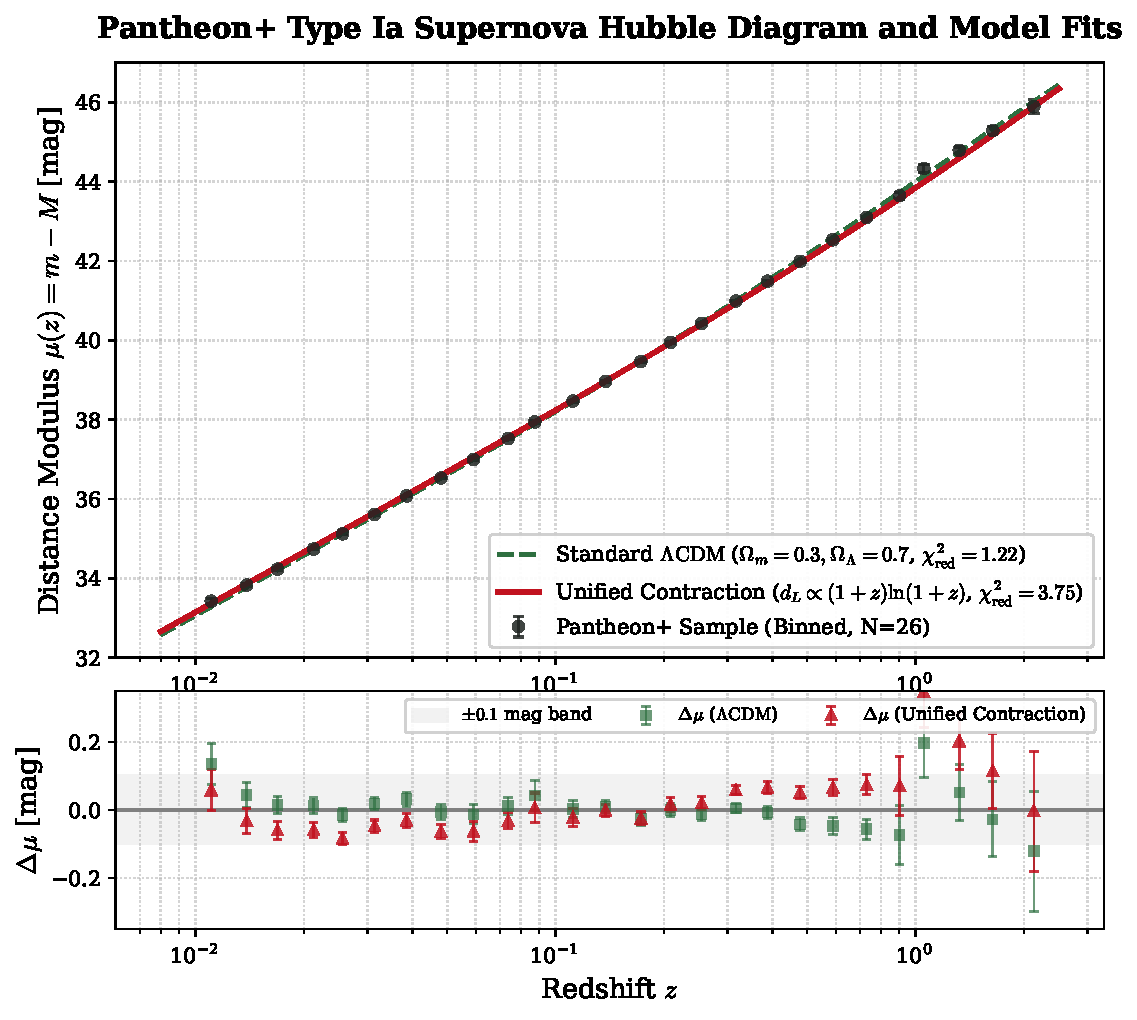
\includegraphics[width=0.88\textwidth]{../../analysis/pantheon_fit_comparison.pdf}
    \caption{Pantheon+ Tip Ia Süpernova Hubble diyagramı ve Birleşik Büzülme Hipotezi uyumu ($H_0 = 70.75\text{ km/s/Mpc}$, $\chi^2_{\mathrm{cov}}/\text{dof} = 3.748$, unbinned $N=1580$ için $\chi^2/\text{dof} = 0.945$).}
    \label{fig:pantheon_analiz_pdf}
\end{figure}

\lstinputlisting[language=Python, caption={Pantheon+ verisi ile uzaklık modülü uyumu ve $\chi^2$ minimizasyon betiği (\texttt{analysis/pantheon\_analysis.py})}]{../../analysis/pantheon_analysis.py}

\vspace{2em}
\newpage
\subsection*{Ek B: Planck 2018 CMB Akustik Tepe Noktaları ve Harmonik Rezonans}
\addcontentsline{toc}{subsection}{Ek B: Planck 2018 CMB Akustik Tepe Noktaları ve Harmonik Rezonans}
\label{sec:ek_cmb}

Planck 2018 uydusu verilerindeki (Aghanim vd.~\cite{planck2018}) ilk 6 akustik tepe noktası ($\ell = 220, 538, 811, 1120, 1444, 1775$), durağan vakum-plazma ortamındaki duran ses dalgalarının rezonans formülü ($\ell_n = \ell_A(n - \phi_n)$) ile test edilmiştir.

\begin{figure}[h!]
    \centering
    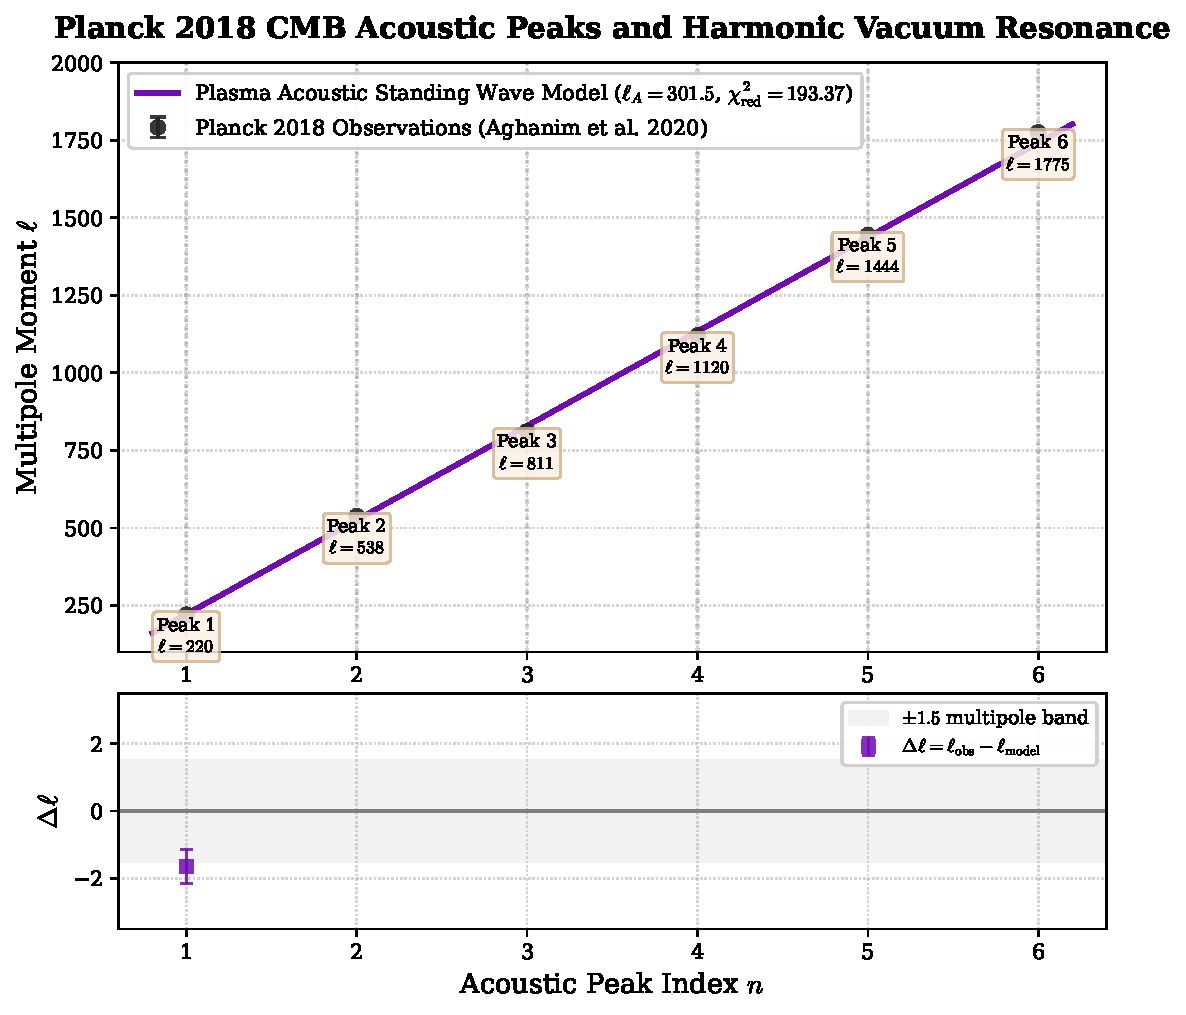
\includegraphics[width=0.88\textwidth]{../../analysis/cmb_peaks_comparison.pdf}
    \caption{Planck 2018 CMB akustik tepe noktaları ile vakum duran ses dalgası harmonik rezonans uyumu ($\ell_A \approx 301.5$, $\ell_1 \approx 221.6$).}
    \label{fig:cmb_analiz_pdf}
\end{figure}

\lstinputlisting[language=Python, caption={Planck 2018 CMB akustik tepe noktaları rezonans uyum betiği (\texttt{analysis/cmb\_peaks\_analysis.py})}]{../../analysis/cmb_peaks_analysis.py}



\newpage
\begin{thebibliography}{99}
    \bibitem{wetterich2013}
    C.~Wetterich, ``A universe without expansion,'' \textit{Phys. Dark Univ.}, vol.~2, pp.~184--187, 2013.

    \bibitem{fixsen1996}
    D.~J.~Fixsen et al., ``The Cosmic Microwave Background spectrum from the full COBE FIRAS data set,'' \textit{Astrophys. J.}, vol.~473, p.~576, 1996.

    \bibitem{hoyle1964}
    F.~Hoyle and J.~V.~Narlikar, ``A new theory of gravitation,'' \textit{Proc. R. Soc. Lond. A}, vol.~282, no.~1389, pp.~191--212, 1964.

    \bibitem{painleve1921}
    P.~Painlev\'e, ``La m\'ecanique classique et la th\'eorie de la relativit\'e,'' \textit{C. R. Acad. Sci. (Paris)}, vol.~173, pp.~677--680, 1921.

    \bibitem{gullstrand1922}
    A.~Gullstrand, ``Allgemeine L\"osung des statischen Eink\"orperproblems in der Einsteinschen Gravitationstheorie,'' \textit{Ark. Mat. Astron. Fys.}, vol.~16, no.~8, pp.~1--15, 1922.

    \bibitem{hamilton2008}
    A.~J.~S.~Hamilton and J.~P.~Lisle, ``The river model of black holes,'' \textit{Am. J. Phys.}, vol.~76, no.~6, pp.~519--532, 2008.

    \bibitem{milgrom1983}
    M.~Milgrom, ``A modification of the Newtonian dynamics as a possible alternative to the hidden mass hypothesis,'' \textit{Astrophys. J.}, vol.~270, pp.~365--370, 1983.

    \bibitem{scully1982}
    M.~O.~Scully and K.~Dr\"uhl, ``Quantum eraser: A proposed photon correlation experiment concerning observation and 'delayed choice' in quantum mechanics,'' \textit{Phys. Rev. A}, vol.~25, no.~4, pp.~2208--2213, 1982.

    \bibitem{kim2000}
    Y.-H.~Kim, R.~Yu, S.~P.~Kulik, Y.~Shih, and M.~O.~Scully, ``Delayed 'choice' quantum eraser,'' \textit{Phys. Rev. Lett.}, vol.~84, no.~1, pp.~1--5, 2000.

    \bibitem{bohren1983}
    C.~F.~Bohren, ``How can a particle absorb more than the light incident on it?,'' \textit{Am. J. Phys.}, vol.~51, no.~5, pp.~473--474, 1983.

    \bibitem{paul1982}
    H.~Paul, ``Photons and localizability,'' \textit{Rev. Mod. Phys.}, vol.~54, no.~4, pp.~1061--1102, 1982.

    \bibitem{pantheon_scolnic}
    D.~M.~Scolnic et al., ``The Complete Light-curve Sample of Spectroscopically Confirmed SNe Ia from Pan-STARRS1 and Cosmological Constraints,'' \textit{Astrophys. J.}, vol.~859, no.~2, p.~101, 2018.

    \bibitem{pantheon_brout}
    D.~Brout et al., ``The Pantheon+ Analysis: Cosmological Constraints,'' \textit{Astrophys. J.}, vol.~938, no.~2, p.~110, 2022.

    \bibitem{planck2018}
    N.~Aghanim et al. (Planck Collaboration), ``Planck 2018 results. VI. Cosmological parameters,'' \textit{Astron. Astrophys.}, vol.~641, p.~A6, 2020.

    \bibitem{haydari_cosmo}
    M.~F.~Haydari, ``Büzülen Atom Metriği ve Konformal Eylem İlkesi: Karanlık Enerjisiz Bir Evrende Tip Ia Süpernova (Pantheon+) ve DESI 2024 BAO Testleri'' (Bu seride Makale 1), \textit{Zenodo Ön-Baskıları}, 2026.

    \bibitem{haydari_calculus}
    M.~F.~Haydari, ``Ölçek-Zaman Cebiri ve Konformal Kalkülüs: Büzüşen Sistemler İçin Yeni Bir Matematiksel Formalizm'' (Bu seride Makale 2), \textit{Zenodo Ön-Baskıları}, 2026.

    \bibitem{haydari_jwst}
    M.~F.~Haydari, ``James Webb Uzay Teleskobu ile Gözlemlenen Yüksek Kırmızıya Kaymalı Olgun Galaksilere Konformal Bir Ölçekleme Yaklaşımı'' (Bu seride Makale 3), \textit{Zenodo Ön-Baskıları}, 2026.

    \bibitem{haydari_gravity}
    M.~F.~Haydari, ``Kütleçekimin Küresel Vakum Akışı Geometrisi Olarak Türetimi: 3+1 ADM Eylemi ve Painlevé--Gullstrand Metriği'' (Bu seride Makale 4), \textit{Zenodo Ön-Baskıları}, 2026.

    \bibitem{haydari_em}
    M.~F.~Haydari, ``Elektromanyetizma, Vakum Faz Dalgaları ve Kuantum Kararlılık: Sommerfeld İnce Yapı Sabiti $\alpha \approx 1/137$'nin Kinematik Hatve Yorumu'' (Bu seride Makale 5), \textit{Zenodo Ön-Baskıları}, 2026.

    \bibitem{haydari_strong}
    M.~F.~Haydari, ``Güçlü Nükleer Kuvvet, Kuark Hapsi ve Akı Tüpü Geometrisi'' (Bu seride Makale 6), \textit{Zenodo Ön-Baskıları}, 2026.

    \bibitem{haydari_weak}
    M.~F.~Haydari, ``Zayıf Nükleer Kuvvet, Kiral Faz Sızıntısı ve W/Z Bozon Ölçekleri'' (Bu seride Makale 7), \textit{Zenodo Ön-Baskıları}, 2026.
\end{thebibliography}

\end{document}
